%% 
%% Copyright 2007-2024 Elsevier Ltd
%% 
%% This file is part of the 'Elsarticle Bundle'.
%% ---------------------------------------------
%% 
%% It may be distributed under the conditions of the LaTeX Project Public
%% License, either version 1.3 of this license or (at your option) any
%% later version.  The latest version of this license is in
%%    http://www.latex-project.org/lppl.txt
%% and version 1.3 or later is part of all distributions of LaTeX
%% version 1999/12/01 or later.
%% 
%% The list of all files belonging to the 'Elsarticle Bundle' is
%% given in the file `manifest.txt'.
%% 
%% Template article for Elsevier's document class `elsarticle'
%% with harvard style bibliographic references

%\documentclass[preprint,12pt,authoryear]{elsarticle}

%% Use the option review to obtain double line spacing
%%\documentclass[authoryear,preprint,review,12pt]{elsarticle}

%% Use the options 1p,twocolumn; 3p; 3p,twocolumn; 5p; or 5p,twocolumn
%% for a journal layout:
%% \documentclass[final,1p,times,authoryear]{elsarticle}
%% \documentclass[final,1p,times,twocolumn,authoryear]{elsarticle}
%% \documentclass[final,3p,times,authoryear]{elsarticle}
%% \documentclass[final,3p,times,twocolumn,authoryear]{elsarticle}
%% \documentclass[final,5p,times,authoryear]{elsarticle}
\documentclass[final,5p,times,twocolumn,authoryear]{elsarticle}

%% For including figures, graphicx.sty has been loaded in
%% elsarticle.cls. If you prefer to use the old commands
%% please give \usepackage{epsfig}

%% The amssymb package provides various useful mathematical symbols
%% The amsmath package provides various useful equation environments.
\usepackage{graphicx}
\usepackage{amsmath,amssymb,amsfonts}
\usepackage{multirow}
\usepackage{mathrsfs}
\usepackage[title]{appendix}
\usepackage{xcolor}
\newcommand{\AUTHORACTION}[1]{\textcolor{red}{\textbf{[AUTHOR ACTION REQUIRED: #1]}}}
%% Placeholder macros for the not-yet-run SOTA/commercial-app comparison (Section~\ref{subsec:sota_comparison}).
%% \TBD marks a single missing table cell; \TODO{...} marks a longer instructional note.
%% Both render in orange so they are easy to grep/spot and MUST be removed before submission.
\newcommand{\TBD}{\textcolor{orange}{\textbf{TBD}}}
\newcommand{\TODO}[1]{\textcolor{orange}{\textbf{[TODO: #1]}}}
\usepackage{textcomp}
\usepackage{manyfoot}
\usepackage{booktabs}
\usepackage{algorithm}
\usepackage{algorithmicx}
\usepackage{algpseudocode}
\usepackage{listings}
\usepackage{float}
\usepackage{tabularx}
\usepackage{subcaption}
\usepackage{enumitem}
\usepackage[ colorlinks=true,linkcolor=blue,citecolor=blue, urlcolor=blue]{hyperref}

%% The amsthm package provides extended theorem environments
%% \usepackage{amsthm}

%% The lineno packages adds line numbers. Start line numbering with
%% \begin{linenumbers}, end it with \end{linenumbers}. Or switch it on
%% for the whole article with \linenumbers.
%% \usepackage{lineno}

\journal{Expert Systems with Applications}

\raggedbottom

\begin{document}

\begin{frontmatter}

%% Title, authors and addresses

%% use the tnoteref command within \title for footnotes;
%% use the tnotetext command for theassociated footnote;
%% use the fnref command within \author or \affiliation for footnotes;
%% use the fntext command for theassociated footnote;
%% use the corref command within \author for corresponding author footnotes;
%% use the cortext command for theassociated footnote;
%% use the ead command for the email address,
%% and the form \ead[url] for the home page:
%% \title{Title\tnoteref{label1}}
%% \tnotetext[label1]{}
%% \author{Name\corref{cor1}\fnref{label2}}
%% \ead{email address}
%% \ead[url]{home page}
%% \fntext[label2]{}
%% \cortext[cor1]{}
%% \affiliation{organization={},
%%            addressline={}, 
%%            city={},
%%            postcode={}, 
%%            state={},
%%            country={}}
%% \fntext[label3]{}

\title{CashVision: A Rule-Governed, Energy-Aware Mobile Expert System for Polymer Banknote Recognition and Tear Detection to Assist Visually Impaired Users}

\author[label1]{Quoc Thai Mai\corref{cor1}}
\cortext[cor1]{Corresponding author}\ead{23133071@student.hcmute.edu.vn}

\author[label1]{Xuan Phi Nguyen}

\author[label2]{Ngoc Tien Ho}
\author[label2]{Gia Toan Nguyen}

\affiliation[label1]{
    organization={Faculty of Information Technology, HCMC University of Technology and Engineering},
    addressline={No. 1 Vo Van Ngan Street, Thu Duc City},
    city={Ho Chi Minh City},
    postcode={700000},
    country={Vietnam}
}

\affiliation[label2]{
    organization={Faculty of Management Information System, Ho Chi Minh City University of Banking},
    addressline={No. 56 Hoang Dieu II Street, Thu Duc City},
    city={Ho Chi Minh City},
    postcode={700000},
    country={Vietnam}
}

%% Abstract
\begin{abstract}
Autonomous banknote verification and defect inspection are essential for the financial independence of visually impaired individuals, yet reflective polymer substrates and unconstrained mobile video handling present substantial operational challenges. Continuous uniform-rate neural inference exhausts mobile battery reserves and induces thermal throttling, whereas an author-implemented timer-triggered single-shot baseline yields low accuracy and frequent valuation errors. We present \textbf{CashVision}, an energy-aware mobile expert system for joint currency denomination recognition and tear defect localization. CashVision integrates an ultra-lightweight parametric tone-mapping module (MQTone) as an inductive preprocessor to mitigate specular glare, coupled with an adaptive execution cascade. Governed by an optical Quality-Gate and a temporal-consensus finite state machine, the system triggers deep inference only upon confirming optical stability. Robustness to adverse illumination was established offline using a multi-condition polymer currency dataset, where the cascade reduced the host computational energy proxy by $61.3\%$. In live trials on a commercial smartphone conducted under everyday ambient indoor lighting, CashVision attained $83.3\%$ verification accuracy without monetary valuation errors, sustained the camera preview cadence of $20.5$\,FPS, and lowered active power draw by $36.5\%$. In an assistive user study with sighted participants under a blindfold protocol, CashVision achieved a System Usability Scale score of $78.2$, reduced subjective workload, and limited the financial hazard rate to $1.0\%$. These results show that rule-governed sensory gating enables dependable, energy-efficient assistive banknote inspection on mobile devices under everyday conditions.
\end{abstract}

%%Graphical abstract
\begin{graphicalabstract}
\begin{center}
\fbox{
  \begin{minipage}[c][6cm][c]{0.95\textwidth}
    \centering
    \textbf{GRAPHICAL ABSTRACT PLACEHOLDER}\\[1em]
    \AUTHORACTION{Replace placeholder with compliant graphical abstract following specifications in figures/graphical\_abstract\_SPEC.md. Generative-AI artwork is prohibited by Elsevier policy; replacement must use exclusively real dataset captures, vector diagrams, and verified Android app screenshots.}
  \end{minipage}
}
\end{center}
\end{graphicalabstract}

%%Research highlights
\begin{highlights}
\item Multi-condition polymer banknote benchmark: 1,812 dual-bbox images, 36 videos.
\item MQTone (19,686 params) automates edge tone conditioning under specular glare.
\item Adaptive cascade cuts host compute energy proxy by 61.3\% in video benchmarks.
\item Smartphone trials: 20.5 FPS preview, 36.5\% active power cut under ambient light.
\item Blindfolded user study: SUS 78.2, 42.3\% lower workload, 1.0\% financial hazard.
\end{highlights}

%% Keywords
\begin{keyword}
%% keywords here, in the form: keyword \sep keyword
Mobile expert system\sep Energy-aware edge inference\sep Real-time object detection\sep Adaptive illumination correction\sep Banknote defect detection\sep Assistive technology for the visually impaired
\end{keyword}

\end{frontmatter}

%% Add \usepackage{lineno} before \begin{document} and uncomment 
%% following line to enable line numbers
%% \linenumbers

%% main text
%%

\section{Introduction}
\label{sec:intro}
 
Globally, at least 2.2 billion people live with vision impairment, including more than 253 million individuals experiencing moderate-to-severe distance visual impairment or total blindness \cite{Bourne2017,WHO2021}. For this population, everyday cash handling and retail transactions represent critical barriers to independent living \cite{Morris2018,Kacorri2017,Vazquez2024}. Unlike sighted individuals who effortlessly verify a banknote's denomination, authenticity, and structural fitness at a glance, visually impaired individuals must rely on indirect tactile or auditory cues, leaving them vulnerable to shortchanging, accidental overpayment, and counterfeit fraud \cite{Hasanuzzaman2012,Dunai2017,AlZuBi2023}. While commercial assistive smartphone applications (e.g., TapTapSee \cite{TapTapSee}, LookTel Money Reader \cite{LookTel}, and Microsoft Seeing AI \cite{SeeingAI}) have emerged, they either rely on static snapshot capture or whole-image classification under uniform lighting, frequently struggling when exposed to unconstrained handheld video handling in daily retail environments \cite{Rao2023,Dhar2024}.

This assistive challenge is compounded by the worldwide adoption of polymer currency (biaxially-oriented polypropylene, BOPP), currently circulated by over 50 central banks globally \cite{vanRenesse2005,deHeij2006}. Although polymer substrates provide superior structural longevity and anti-counterfeiting security relative to traditional cotton-paper bills, their non-porous, specularly reflective surfaces---integrated with transparent diffractive optical windows---frequently trigger specular glare, flare streaks, and localized sensor saturation under standard ambient lighting, obscuring denomination numerals and tactile watermarks \cite{vanRenesse2005,deHeij2006,Fu2023,Wu2024}. Concurrently, polymer bills are susceptible to tear propagation along substrate fold lines, and physically torn notes are routinely rejected by automated teller machines (ATMs) and point-of-sale vendors. A dependable mobile assistive expert system must therefore do more than output a coarse denomination label: it must execute \textit{joint currency denomination recognition and physical tear defect localization} in real time to alert users before invalid tender is transacted \cite{Pham2017,Pham2018,Dhar2024,Chen2024}.

Transitioning deep-learning object detectors \cite{Redmon2016,Bochkovskiy2020,Jocher2023} and lightweight convolutional backbones \cite{Howard2019,Sandler2018,Tan2021} from curated image databases to continuous mobile video reveals a critical \textit{Static-to-Video Deployment Gap}. Existing mobile assistive pipelines face an operational trade-off:
\begin{enumerate}[label=(\alph*)]
    \item \textbf{Naive Uniform-Rate Processing ($B_0$):} Executing full neural inference on every incoming raw frame ($30$\,FPS) theoretically minimizes algorithmic misses but causes excessive energy dissipation ($\approx 600$\,J per session based on an estimated host CPU active compute proxy at $\sim 22$\,W, and $130.5$\,J on mobile hardware) alongside severe thermal throttling on mobile System-on-Chips (SoCs) \cite{Ignatov2018,Lane2016}, resulting in execution queue backpressure, frame drops, and palm discomfort precisely when responsive guidance is required.
    \item \textbf{Timer-Triggered Single-Shot Baseline ($B_1$):} To model conventional snapshot capture without continuous video monitoring, we implement a timer-triggered single-shot baseline that executes detection after a pre-programmed delay (e.g., $t = 1.0$\,s). In continuous handheld video streams, this baseline achieves only $8.3\%$ exact-match accuracy ($52.8\%$ in live smartphone trials). Because visually impaired users cannot visually align the smartphone viewfinder, hand tremor, dynamic velocity blur, and border occlusions corrupt static captures. In physical smartphone trials, this single-shot baseline incurs a $14.6\%$ financial hazard rate, generating substantial 20- to 25-fold monetary valuation errors (e.g., mistaking a $200{,}000$\,VND note for $10{,}000$\,VND, or a $20{,}000$\,VND note for $500{,}000$\,VND) that inflict serious economic consequences.
\end{enumerate}

Developing an autonomous, on-device mobile assistive expert system therefore demands resolving three fundamental limitations spanning the literature:
\begin{itemize}
    \item \textbf{Limitations in Mobile Assistive Currency Recognition:} First-generation systems relied on handcrafted keypoint descriptors (SIFT, SURF, AdaBoost) \cite{Hasanuzzaman2012,Dunai2017}, which were computationally prohibitive for real-time video and fragile to affine perspective distortion. Contemporary mobile applications rely on cloud-based visual search \cite{TapTapSee,Kacorri2017} that incurs prohibitive $3$--$10$\,s round-trip latency and fails without network connectivity. While recent studies have successfully deployed modern YOLO architectures (e.g., YOLOv8, YOLOv9, YOLOv10) for assistive fiat banknote recognition \cite{AlZuBi2023,Dhar2024,Ghanem2025}---such as the real-time Egyptian currency identification system by \citet{Ghanem2025}---these investigations focus on static image datasets of diffuse cotton-paper currency under controlled or stationary capture, leaving unaddressed the non-Lambertian specular reflections of polymer substrates, localized structural tear defects, and the energy/thermal constraints of continuous real-time video streaming on edge SoCs.
    \item \textbf{Limitations in Banknote Fitness and Defect Inspection:} Existing fitness screening techniques \cite{Ahmadi2004,Lee2017,Gai2013,Pham2018,Yuan2023,Chen2024} are engineered primarily for industrial central-bank sorting machines. These systems presuppose rigid motorized conveyor belts and calibrated multi-spectral illumination (infrared, ultraviolet, polarized), yielding only binary fit/unfit classifications. They cannot operate on handheld RGB video streams or provide fine-grained spatial defect localization.
    \item \textbf{Limitations in On-Device Photometric Enhancement:} Classical enhancement algorithms (Gamma correction \cite{Gonzalez2008}, CLAHE \cite{Zuiderveld1994}) apply spatially uniform remapping that washes out specular highlights or amplifies high-frequency substrate noise. Modern learning-based enhancers (Zero-DCE \cite{Guo2020}, Zero-DCE++ \cite{Li2021}, and IAT \cite{Cui2022}) are formulated to brighten underexposed nocturnal scenes; when exposed to overexposed polymer banknotes, their monotonic curve mappings amplify specular blowout and obscure delicate guilloche printing (driving Zero-DCE++ accuracy down to $56.3\%$), while heavy transformer architectures \cite{Cui2022,Cai2023} exceed mobile real-time compute envelopes \cite{Huang2023,Zhang2024,Li2023}.
\end{itemize}

Autonomous banknote verification and physical defect inspection for visually impaired individuals in unconstrained retail environments represent a high-stakes decision problem under severe physical uncertainty: non-porous polymer substrates generate intense specular glare and conceal structural tear fractures, while users handle cash without visual viewfinder feedback, introducing hand tremor, perspective tilt, and dynamic motion blur. In such handheld edge deployments, executing deep neural inference continuously across incoming video frames rapidly exhausts battery reserves and triggers thermal throttling, whereas naive single-shot snapshotting incurs dangerous monetary valuation errors. Resolving this operational conflict requires a rule-governed expert arbitration architecture: a decision layer that continuously monitors sensory readiness, gates deep computational execution to preserve thermal and energy autonomy, and accumulates multi-frame temporal consensus before committing to an irreversible financial recommendation. Within this expert system framework, specialized neural sub-networks serve targeted sensory functions under meta-level control: MQTone adaptively normalizes localized specular overexposure and contrast degradation via parametric curve prediction without manual calibration, while a dual-task YOLOv8n detector concurrently identifies currency denomination and localizes physical tear fractures on demand. When integrated into a fully offline mobile application on a commercial Samsung Galaxy A54 smartphone and evaluated with blindfolded participants under simulated visual impairment ($N=16$, $288$ trials), CashVision achieves $83.3\%$ live verification accuracy with zero monetary valuation errors ($0/36$), sustains an uninterrupted $20.5$\,FPS preview cadence while reducing active power draw by $36.5\%$, and decreases cognitive workload by $42.3$--$53.0\%$ while maintaining a low $1.0\%$ financial hazard rate.

The principal contributions of this work are summarized as follows:
\begin{enumerate}[label=\textbf{(C\arabic*)}]
    \item \textbf{Multi-Condition Polymer Benchmark and Problem Characterization:} We establish a multi-condition polymer currency benchmark comprising $1{,}812$ dual-annotated images (denomination boxes and localized tear fractures) and $36$ continuous handheld video streams ($9{,}060$ frames total) across six operational environments. We systematically characterize the cross-condition degradation of lightweight mobile detectors across circulating banknote captures, showing that denomination classification exhibits marked vulnerability to specular glare (dropping by up to $-12.53$ percentage points) due to surface pixel saturation over planar intaglio patterns, whereas physical substrate tears retain detectable macroscopic boundary discontinuities across color channels.
    \item \textbf{Edge Photometric Conditioning Module (MQTone):} To condition adverse optical frames for the downstream detector without manual parameter tuning, we implement MQTone ($19{,}686$ parameters, $<0.1$\,MB ONNX footprint), an ultra-compact parametric tone-mapping component serving as an inductive preprocessor within the cascade pipeline. In 5-fold cross-validation measuring cross-condition photometric invariance across adverse lighting regimes, MQTone provides an automated parameter estimation front-end that improves overexposure denomination accuracy by $+7.73$ percentage points over an unenhanced detector baseline ($69.63\%$ vs.\ $61.90\%$) and avoids the highlight blowout characteristic of low-light enhancers, integrating into the mobile cascade at $23.2$\,ms mobile CPU latency.
    \item \textbf{Adaptive On-Device Cascade and Physical Smartphone Deployment:} We design an energy-aware cascade pipeline driven by an ultra-lightweight Quality-Gate and a 3-state temporal consensus FSM. Evaluated across an offline continuous video benchmark ($36$ streams, $9{,}060$ frames, cutting host compute energy proxy by $61.3\%$) and live on-device field trials ($36$ interactive camera sessions per paradigm, $108$ physical runs total, over $47{,}000$ processed frames across paradigms) running $100\%$ offline on a Samsung Galaxy A54 via native ONNX Runtime C++ under everyday ambient lighting, CashVision achieves $83.3\%$ verification accuracy with zero monetary valuation errors ($0/36$, 95\% Wilson CI: $[0.0\%, 9.6\%]$, safely deferring unaligned frames), sustains the camera preview cadence of $20.5$\,FPS by avoiding compute-bound inference bottlenecks (vs.\ $3.2$\,FPS for $B_0$), reduces amortized frame compute latency by $97.9\%$ ($6.5$\,ms vs.\ $308.1$\,ms), and lowers active power draw by $36.5\%$ ($2.79$\,W vs.\ $4.39$\,W, with $34.6\%$ session energy savings), preventing SoC thermal throttling.
    \item \textbf{Human-in-the-Loop Usability and Assistive Safety Validation:} We conduct an empirical user study with $N=16$ blindfolded participants across $288$ clustered interactive retail trials under a standardized simulated visual impairment protocol. Generalized Linear Mixed Models (GLMM) and Repeated-Measures ANOVA confirm that CashVision elevates usability to a System Usability Scale (SUS) score of $78.2 \pm 6.9$ (Grade B / ``Good''), reduces NASA-TLX cognitive workload by $42.3\%$ compared to $B_0$ ($53.0\%$ compared to the single-shot baseline $B_1$), accelerates interaction time-to-confirmation by $47.9\%$ in live assistive trials ($5.64$\,s vs.\ $10.82$\,s), and limits the assistive financial hazard rate to $1.0\%$ ($1/96$, vs.\ $14.6\%$ for the single-shot baseline, matching $B_0$'s $4.2\%$ without its latency and thermal costs), demonstrating effective assistive utility in daily retail transactions.
\end{enumerate}

The remainder of this article is structured as follows: Section~\ref{sec:methodology} details the CashVision system architecture, including the dataset structure, expert rule base, MQTone formulation, the dual-task YOLOv8n detector, and the Temporal Consensus FSM; Section~\ref{sec:experiments} presents the experimental setup, static cross-validation results, ablation studies, rule sensitivity analysis, specimen-disjoint evaluation protocol, and state-of-the-art banknote system comparisons; Section~\ref{sec:video_evaluation} analyzes the continuous video benchmarks, physical smartphone telemetry, and simulated visual impairment user study; Section~\ref{sec:conclusion} concludes the paper and outlines future directions for mobile assistive expert systems.

\section{Materials and Proposed Methods}
\label{sec:methodology}

\subsection{Multi-Condition Polymer Banknote Dataset}
\label{subsec:dataset}

\paragraph{Physical Properties and Environmental Taxonomy}
Modern polymer banknotes (biaxially-oriented polypropylene, BOPP) feature smooth, non-porous surfaces, transparent security windows, and micro diffraction optical gratings~\cite{vanRenesse2005}. While highly durable, their reflective properties trigger severe specular glare and sensor saturation under mobile cameras, while substrate fatigue causes physical tears along folds. Rather than relying on sanitized laboratory setups, tripods, or flatbed scanning, our benchmark was collected entirely through natural, unconstrained handheld capture using a Samsung Galaxy A54 smartphone to faithfully mirror real-world assistive conditions. Banknotes were presented naturally in users' hands, incorporating genuine everyday variations such as arbitrary working distances (15--45\,cm), perspective tilts, partial finger occlusions along banknote borders, and diverse background surfaces (counters, tables, domestic textiles). The resulting dataset comprises 1,812 static images and 36 continuous handheld video streams ($9{,}060$ frames at $30$\,FPS) across all six circulating Vietnamese polymer denominations (10, 20, 50, 100, 200, and 500k VND). As detailed in Table~\ref{tab:dataset_distribution}, the data encompasses six operational environments: standard indoor (diffused LED/fluorescent), outdoor sunlight with directional shadows, strong backlighting against bright windows, severe specular overexposure (flash/lamp glare), clean physical tears, and glare-degraded tears on worn banknotes (representative visual examples illustrating these challenges are shown in Figure~\ref{fig:dataset_samples}).

\begin{figure*}[t]
\centering
\begin{subfigure}[b]{0.32\textwidth}
  \centering
  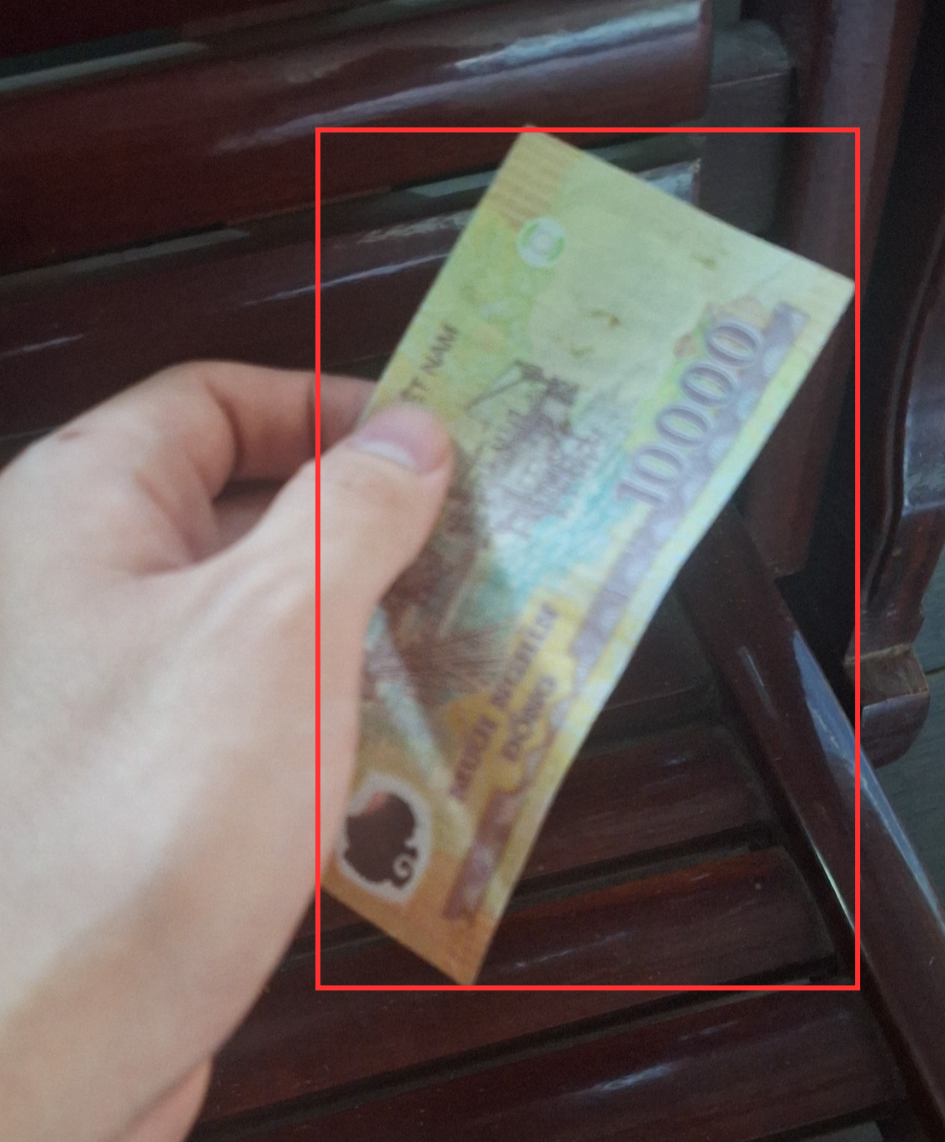
\includegraphics[width=\textwidth,height=3.2cm,keepaspectratio]{train_10k_indoor_0008.png}
  \caption{Indoor Baseline ($10{,}000$\,VND)}
  \label{fig:sample_indoor}
\end{subfigure}\hfill
\begin{subfigure}[b]{0.32\textwidth}
  \centering
  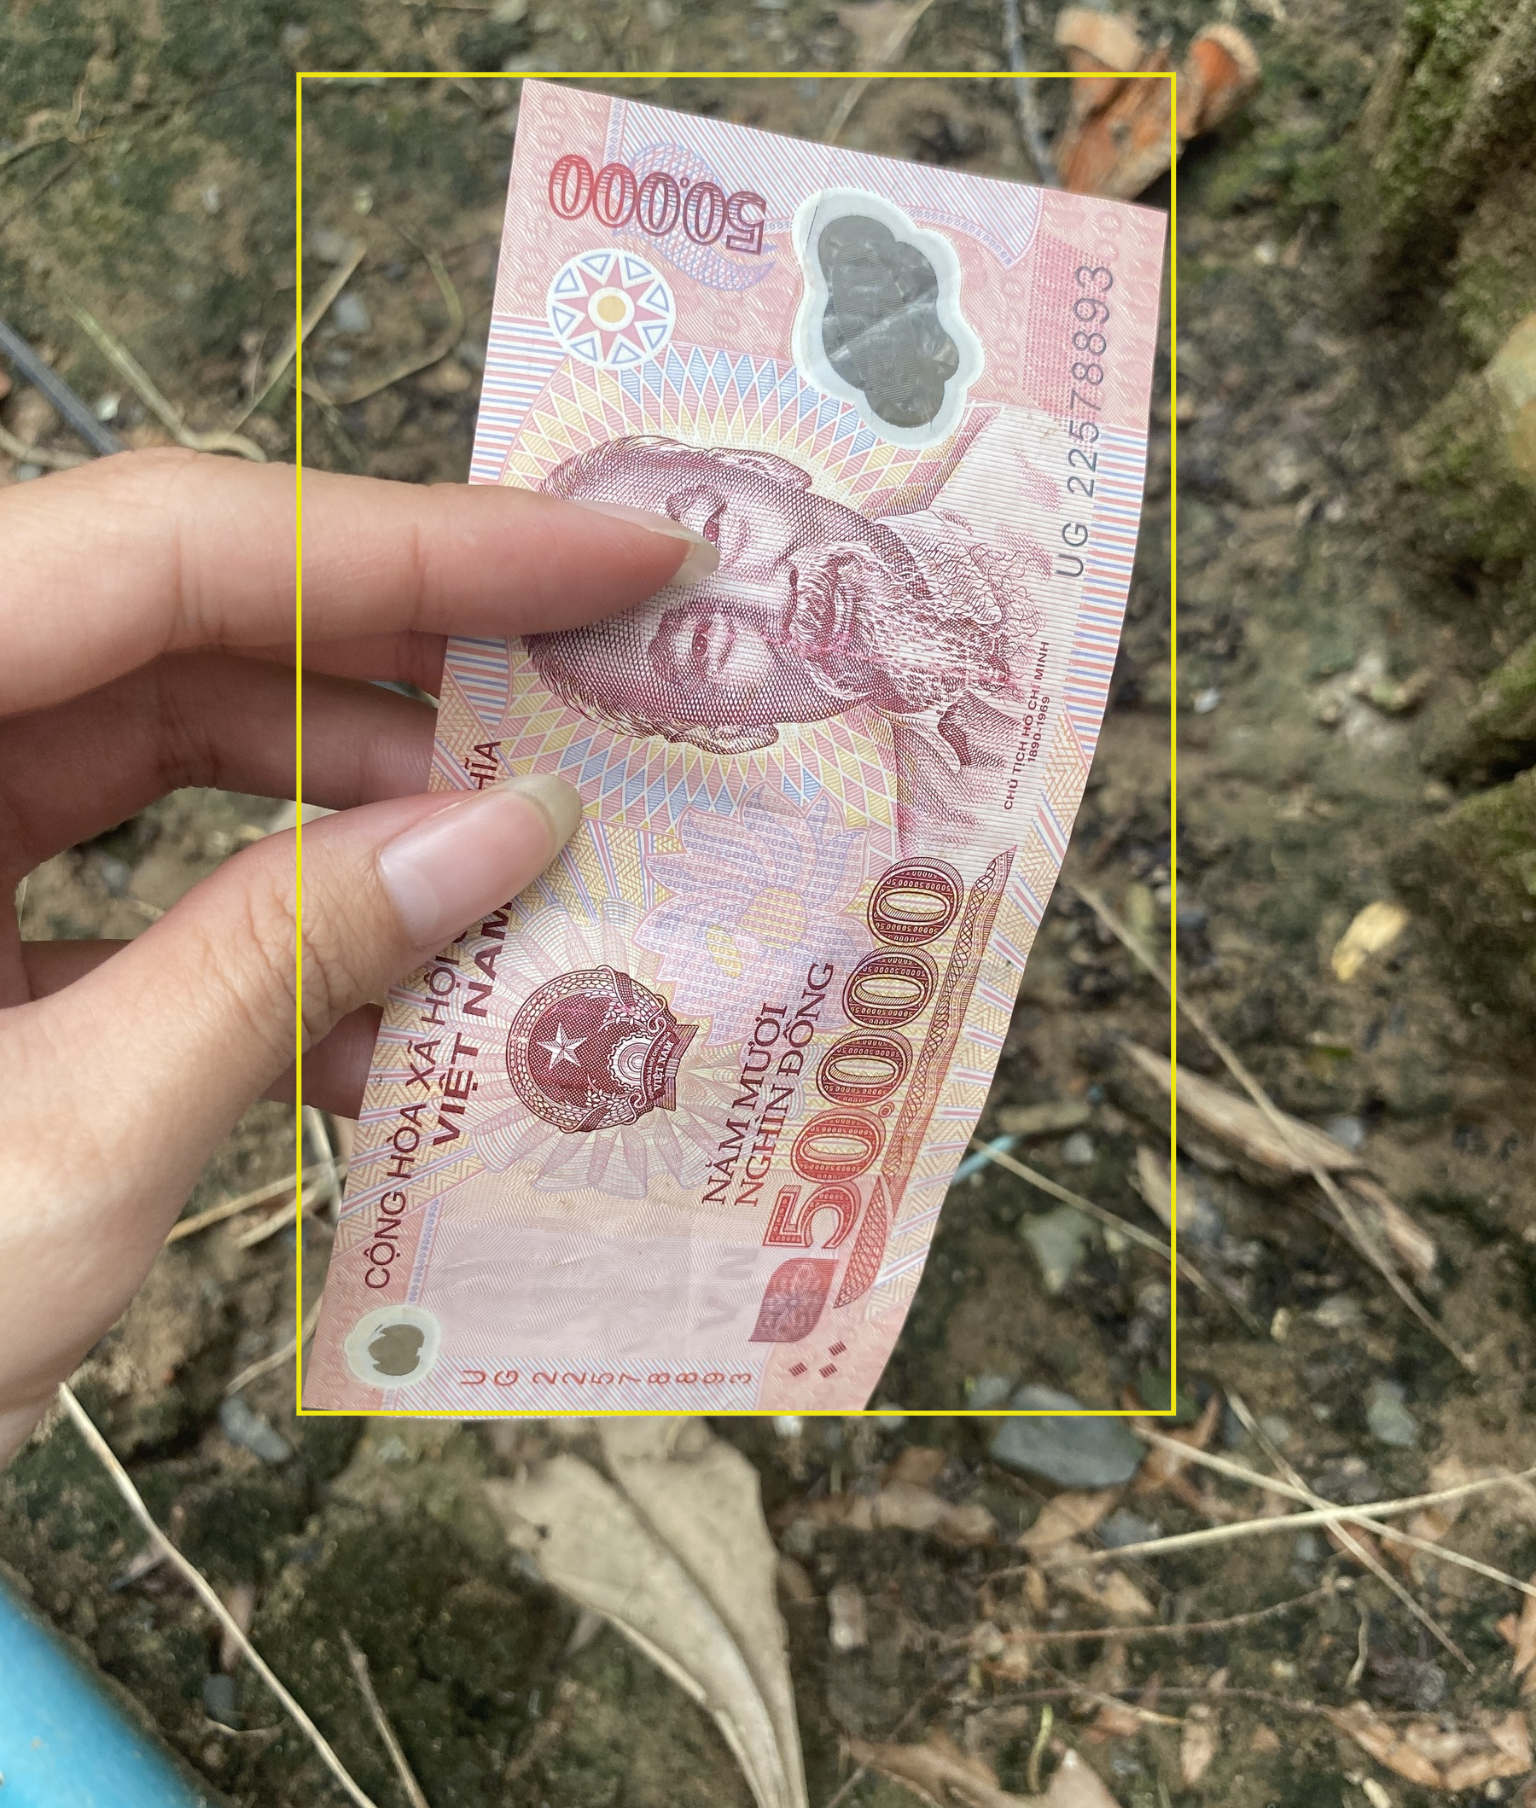
\includegraphics[width=\textwidth,height=3.2cm,keepaspectratio]{train_50k_outdoor_0038.png}
  \caption{Outdoor Sunlight ($50{,}000$\,VND)}
  \label{fig:sample_outdoor}
\end{subfigure}\hfill
\begin{subfigure}[b]{0.32\textwidth}
  \centering
  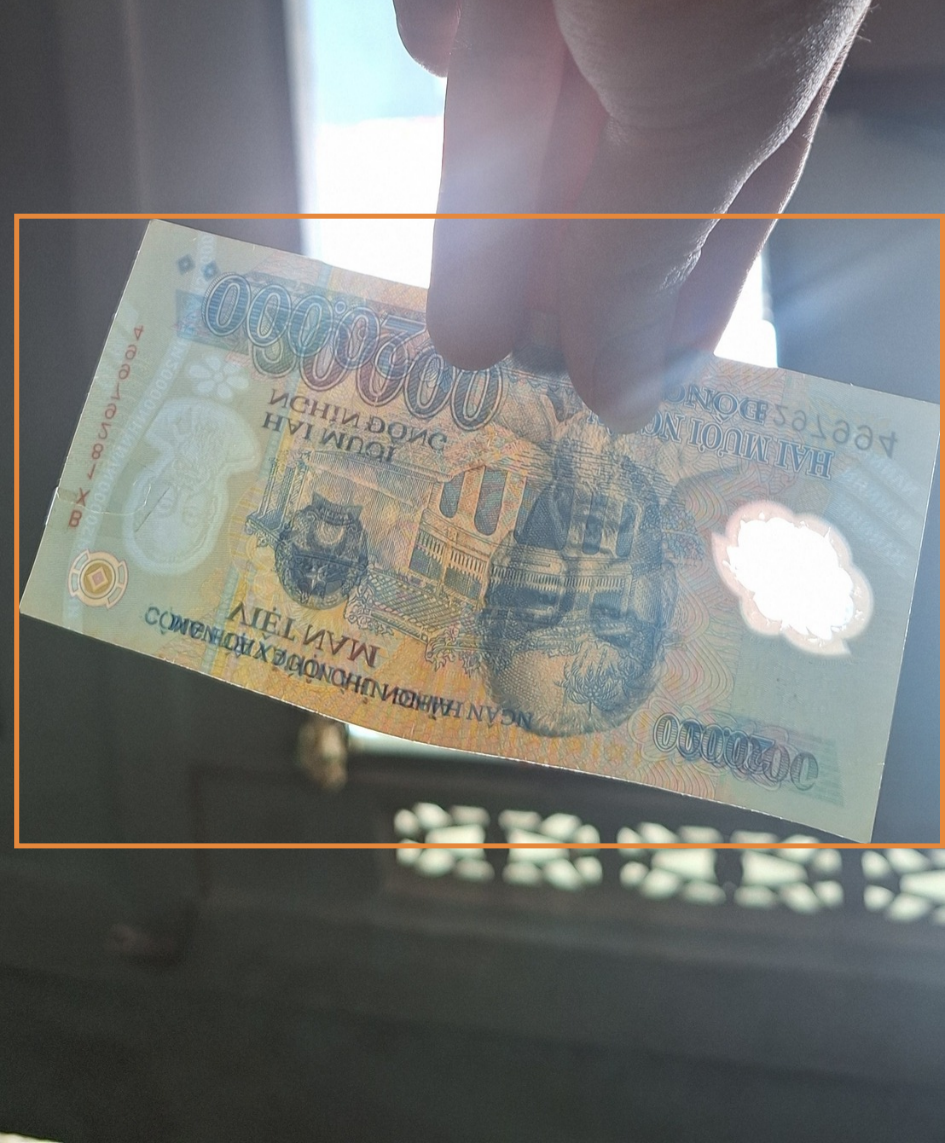
\includegraphics[width=\textwidth,height=3.2cm,keepaspectratio]{train_20k_backlight_0014.png}
  \caption{Strong Backlight ($20{,}000$\,VND)}
  \label{fig:sample_backlight}
\end{subfigure}

\vspace{0.2cm}
\begin{subfigure}[b]{0.32\textwidth}
  \centering
  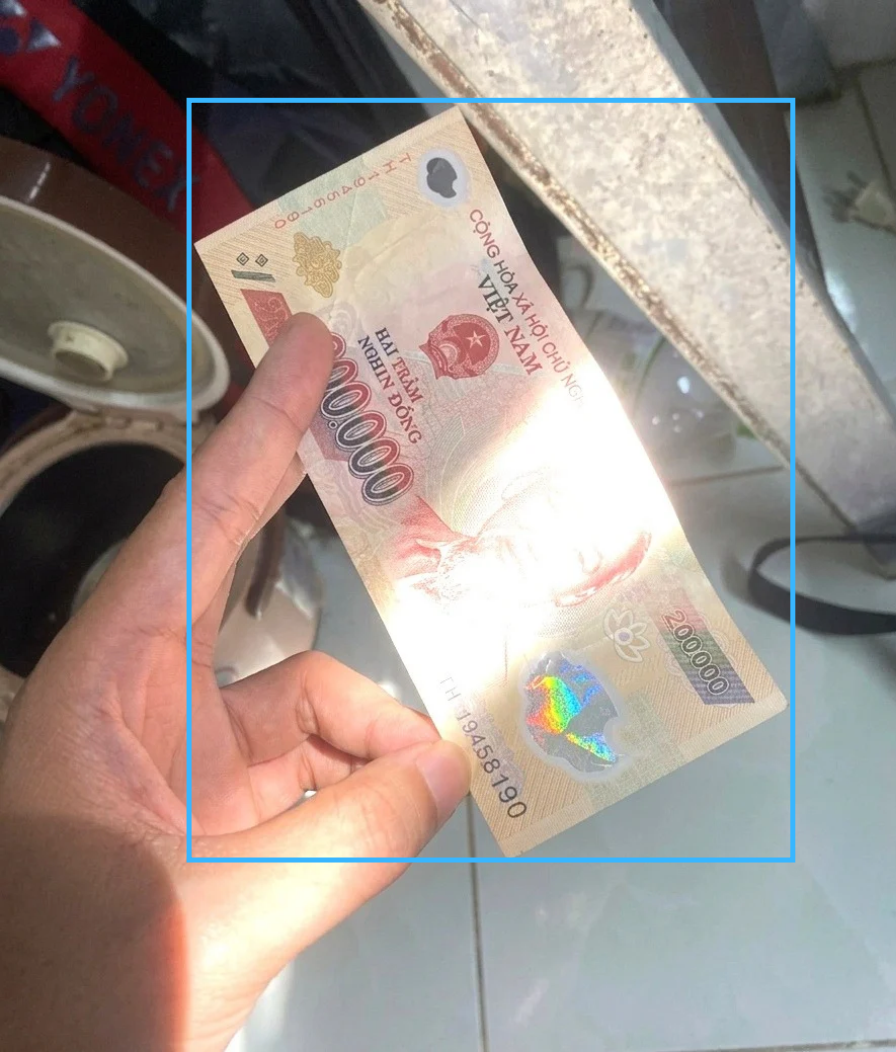
\includegraphics[width=\textwidth,height=3.2cm,keepaspectratio]{train_200k_overexposed_0019.png}
  \caption{Specular Glare ($200{,}000$\,VND)}
  \label{fig:sample_overexposed}
\end{subfigure}\hfill
\begin{subfigure}[b]{0.32\textwidth}
  \centering
  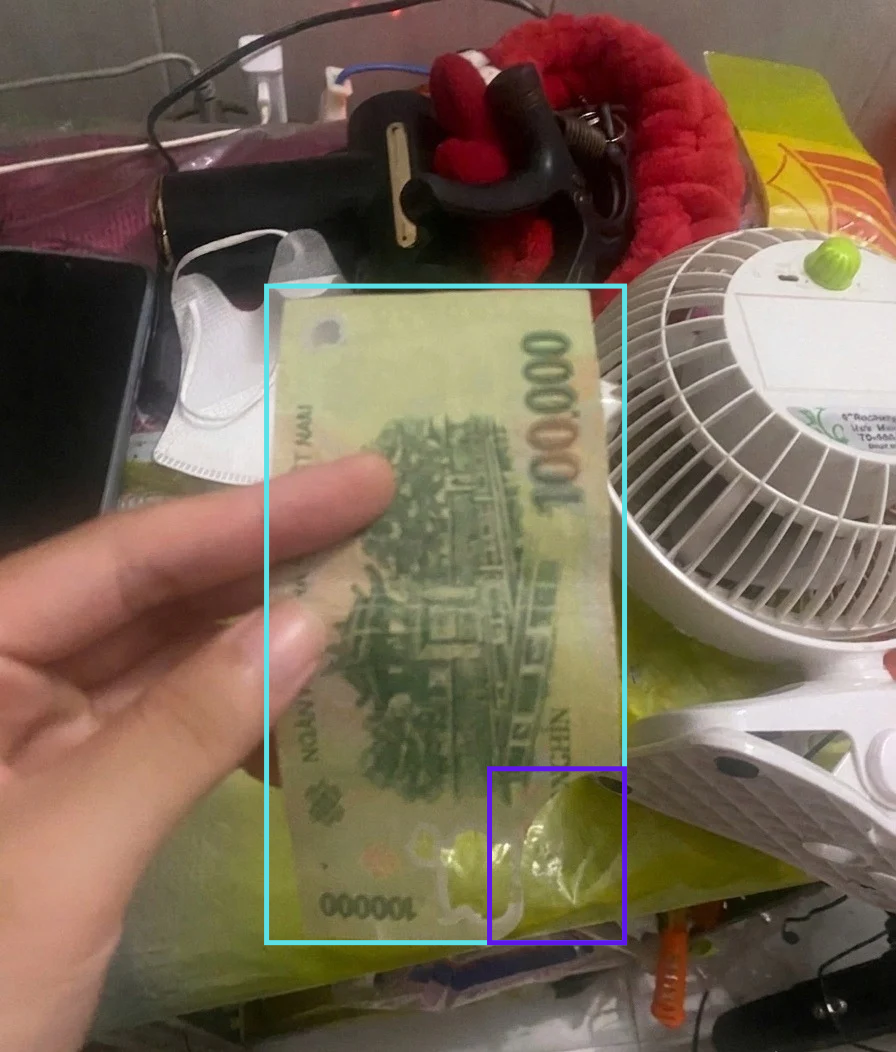
\includegraphics[width=\textwidth,height=3.2cm,keepaspectratio]{train_100k_torn_clean_0021.png}
  \caption{Clean Structural Tear ($100{,}000$\,VND)}
  \label{fig:sample_torn_clean}
\end{subfigure}\hfill
\begin{subfigure}[b]{0.32\textwidth}
  \centering
  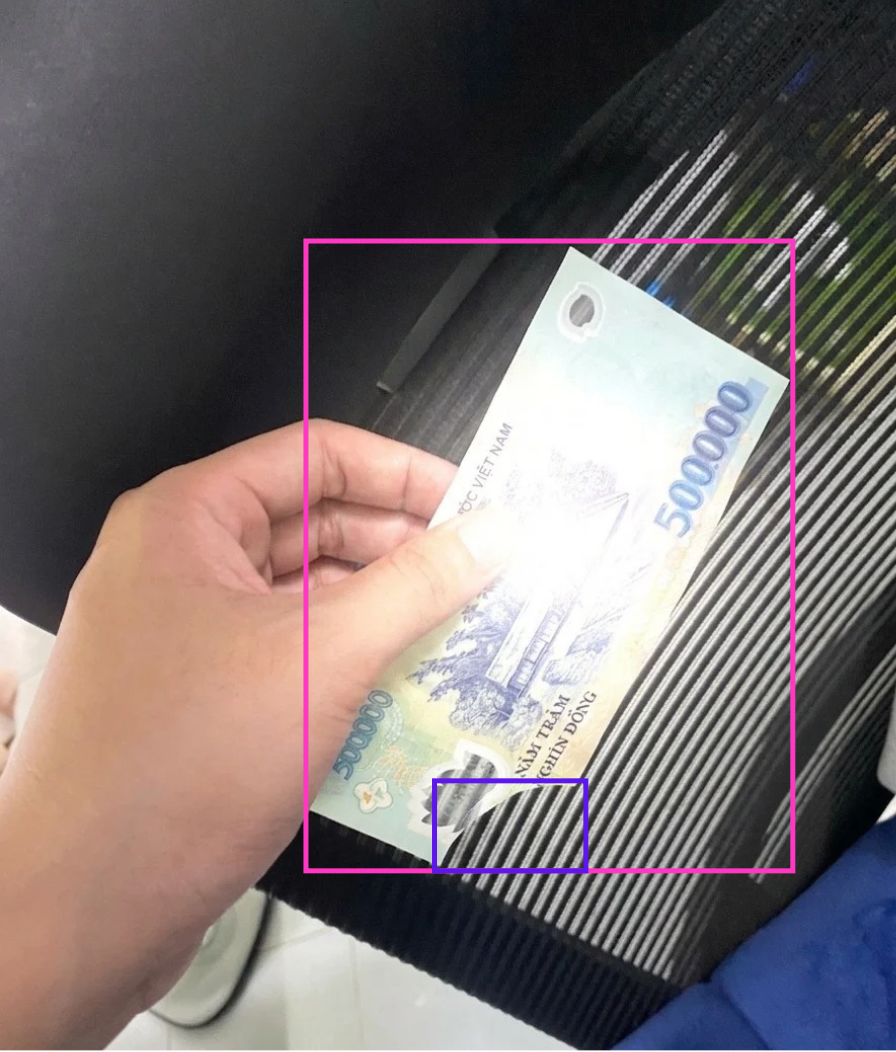
\includegraphics[width=\textwidth,height=3.2cm,keepaspectratio]{train_500k_torn_overexposed_0015.png}
  \caption{Glare Tear ($500{,}000$\,VND)}
  \label{fig:sample_torn_glare}
\end{subfigure}
\caption{Representative sample images from the Multi-Condition Polymer Banknote Benchmark captured on a Samsung Galaxy A54 smartphone under unconstrained real-world handling: (a) indoor baseline, (b) outdoor directional sunlight and shadows, (c) low-contrast backlighting against bright windows, (d) severe specular flash glare on BOPP polymer substrate, (e) structural tear defect, and (f) structural tear confounded by specular reflections.}
\label{fig:dataset_samples}
\end{figure*}

\paragraph{Dataset Composition and Dual-Level Annotation}
The static benchmark comprises 302 images per denomination, totaling 1,812 high-resolution images uniformly structured across all six circulating Vietnamese polymer denominations (10, 20, 50, 100, 200, and 500k VND). As summarized in Table~\ref{tab:dataset_distribution}, each denomination includes intact banknotes (232 images) and structurally damaged notes (70 images) distributed across the operational lighting regimes. To accurately reflect authentic operational variability, images were acquired across distinct physical banknote specimens per denomination over multiple recording sessions, incorporating natural hand tilts, distances (15--45\,cm), finger occlusions, and background surfaces. Notably, the $210$ clean structural tear images ($\texttt{torn\_clean}$) and $210$ glare-degraded tear images ($\texttt{torn\_bright}$) represent the identical physical damaged banknote specimens photographed first under neutral ambient illumination and subsequently under directional flash/specular glare, establishing an optically controlled experimental pair that isolates the confounding impact of specular reflection on defect boundary localization.

Dual-level bounding-box ground truth was annotated using the Roboflow platform: (i) full banknote bounding boxes classifying currency denomination, and (ii) fine-grained defect bounding boxes isolating and localizing the physical tear position and damaged region ($\texttt{torn}$).

The static dataset is partitioned into a canonical structure comprising a training pool of $1{,}260$ images ($69.5\%$, comprising $270$ indoor, $270$ outdoor, $210$ backlight, $210$ overexposed, $150$ torn-clean, and $150$ torn-bright images), an independent validation set of $276$ images ($15.2\%$), and an independent test set of $276$ images ($15.2\%$), yielding a combined held-out evaluation pool of $552$ images ($30.5\%$).

\begin{table}[!tb]
\centering
\caption{Distribution of the Multi-Condition Polymer Banknote Benchmark across operational conditions and note states ($1{,}812$ static images total).}
\label{tab:dataset_distribution}
\scriptsize
\setlength{\tabcolsep}{3pt}
\renewcommand{\arraystretch}{1.15}
\begin{tabular}{llcc}
\toprule
\textbf{Condition Taxonomy} & \textbf{State} &
\textbf{Per Denom ($1\times$)} & \textbf{Total ($6\times$)} \\
\midrule
Standard Indoor & Intact & 65 & 390 \\
Outdoor Sunlight & Intact & 65 & 390 \\
Strong Backlighting & Intact & 51 & 306 \\
Specular Overexposure & Intact & 51 & 306 \\
Clean Structural Tears & Torn & 35 & 210 \\
Glare-Degraded Tears & Torn & 35 & 210 \\
\midrule
\textbf{Total Static Images} & --- & \textbf{302} & \textbf{1,812} \\
\bottomrule
\end{tabular}
\end{table}

\paragraph{Continuous Handheld Video Benchmark}
To assess dynamic streaming performance under unconstrained real-world handling, we recorded 36 continuous handheld video streams (7.0--9.5\,s each, spanning all 6 denominations $\times$ 6 conditions, totaling $9{,}060$ frames at $30$\,FPS) using the same device. Captured under unconstrained user handling, these streams incorporate natural real-world perturbations---including hand tremor, motion blur, angular rotations ($0^\circ$--$180^\circ$), and progressive framing entries/exits. We emphasize that this 36-video streaming benchmark was evaluated on a personal computer (host PC powered by an Intel Core i7-1265U CPU @ 1.80\,GHz, 10 cores, 16\,GB RAM, Windows 11) using a software CPU-load proxy model to provide a reproducible computational benchmark across alternative streaming paradigms, while physical on-device power and energy metrics were independently profiled on smartphone hardware (Section~\ref{subsec:exp_smartphone_deployment}).

\subsection{Proposed Real-Time CashVision Expert System Architecture}
\label{subsec:architecture}

Autonomous banknote verification on mobile edge hardware constitutes a high-stakes decision-making task operating under severe physical uncertainty, battery limitations, and strict thermal envelopes ($<3.0$\,W). In assistive settings, the system must deliver responsive acoustic and haptic guidance within an interactive turnaround latency threshold ($T_{\text{turnaround}} \le 1.5$\,s) \cite{Nielsen1993,Miller1968,Rao2023} once a stable presentation is detected, while maintaining real-time video streaming throughput ($T_{\text{frame}} \le 33.3$\,ms at $30$\,FPS). Rather than treating currency inspection as an unguided end-to-end neural classification task, \textbf{CashVision} is engineered as a canonical expert system that decouples sensory perception from rule-governed decision arbitration and computational resource control.

Structurally, the CashVision expert system architecture decomposes into four classical expert-system pillars:
\begin{enumerate}[label=(\roman*)]
    \item \textbf{Knowledge Base (KB):} An explicit declarative repository of domain facts, physical invariants, and operational thresholds, formalized as rules $R_1$--$R_8$ in Table~\ref{tab:expert_rule_base}. The knowledge base codifies physical properties of polymer substrates (specular reflectance and tear propagation), statistical image luminance distributions, mobile human-computer interaction (HCI) response-time ceilings, and detector confidence baselines.
    \item \textbf{Inference Engine:} A stateful forward-chaining reasoning engine comprising a three-state Finite State Machine (FSM: $\texttt{SEARCHING}$, $\texttt{READY\_TO\_VERIFY}$, and $\texttt{CONFIRMED}$) coupled with multi-frame confidence-weighted voting. The inference engine continuously evaluates video-buffer observations against the rule base, arbitrates hypothesis uncertainty, and deduces confirmed currency denominations and defect classifications.
    \item \textbf{Meta-Level Control:} An energy-aware execution supervisor that dynamically regulates the invocation of compute-intensive neural sub-networks (MQTone and dual-task YOLOv8n). By evaluating zero-inference and micro-classification sensory preconditions prior to dispatching deep inference, meta-level control restricts full execution to stable, informative frames, mitigating mobile SoC thermal throttling and preserving battery autonomy.
    \item \textbf{Explanation Facility:} A translative multimodal user interface that converts internal verified states into transparent, interpretable guidance for the visually impaired user. The facility utilizes speech synthesis (Android TTS) to communicate verified currency values and structured haptic feedback (differentiated single vs.\ dual vibrational pulses) to convey physical structural integrity (intact vs.\ torn defect alerts).
\end{enumerate}

\begin{table*}[t]
\centering

\caption{The CashVision Knowledge Base: Formal Rule Set Governing Sensory Screening, State Transitions, Detection Arbitration, and Decision Explanation.}
\label{tab:expert_rule_base}
\footnotesize
\renewcommand{\arraystretch}{1}
\setlength{\tabcolsep}{3pt}
\begin{tabularx}{\textwidth}{lp{2.6cm}p{4.2cm}p{4cm}p{6cm}}
\toprule
\textbf{Rule} & \textbf{Functional Role} & \textbf{Antecedent / Logical Condition} & \textbf{Consequent / Operational Action} & \textbf{Knowledge Source \& Rationale} \\
\midrule
$R_1$ & Spatial Texture Gating & $\sigma_{\text{gray}} \le \theta_{\text{texture}}$ \newline ($\theta_{\text{texture}} = 15.0$) & Assert $\text{has\_note} = \text{False}$; suppress inference; remain in $\texttt{SEARCHING}$. & \textbf{Photometric physics \& texture entropy:} Featureless non-target frames (pockets, blank tables) exhibit minimal luminance variance \cite{Haralick1979,Gonzalez2008}. \\
$R_2$ & Photometric Readiness & $q < \tau$ ($\tau = 0.60$) or \newline $\mathbb{I}_{\text{degraded}} = \text{True}$ ($q < 0.40$) & Invalidate optical readiness; reset $c_{\text{stable}} \leftarrow 0$; suppress inference. & \textbf{Empirical calibration (dev set):} Severe specular overexposure or underexposure degrades detector feature maps beyond operational reliability. \\
$R_3$ & Temporal Stability & $(\sigma_{\text{gray}} > \theta_{\text{texture}}) \land (q \ge \tau)$ \newline for $c_{\text{stable}} \ge K_{\text{opt}}$ ($K_{\text{opt}} = 3$) & Transition FSM: $\texttt{SEARCHING} \to \texttt{READY\_TO\_VERIFY}$; open verification window. & \textbf{HCI latency \& motor tremor:} A 3-frame ($\approx 100$\,ms) dwell filters transient hand tremor while bounding turnaround well within the $1.5$\,s interactive ceiling \cite{Nielsen1993}. \\
$R_4$ & Verification Budget (Thermal Guard) & Active verification attempts $m \ge M_{\text{verify}}$ ($M_{\text{verify}} = 2$) without consensus & Terminate burst; reset $c_{\text{stable}} \leftarrow 0$; transition FSM back to $\texttt{SEARCHING}$. & \textbf{HCI turnaround \& mobile thermal budget:} Caps active neural compute ($\le 2 \cdot T_{\text{Full}} \approx 616$\,ms), preventing continuous load, thermal throttling, and palm heating. \\
$R_5$ & Candidate Filtering & Detection box confidence $\text{conf}(b) < \theta_{\text{conf}}$ ($\theta_{\text{conf}} = 0.25$) & Discard bounding box $b$ as noise; exclude from consensus voting. & \textbf{Ultralytics detection default:} Standard post-NMS detection confidence threshold for YOLO architectures \cite{Jocher2023}. \\
$R_6$ & Denomination Consensus & Detections in $\mathcal{T}_{\text{verify}}$ yield \newline $c^* = \arg\max_c \sum_{t} s_c^{(t)}$ & Finalize denomination $c^*$; transition FSM: $\texttt{READY\_TO\_VERIFY} \to \texttt{CONFIRMED}$. & \textbf{Evidence accumulation theory:} Multi-frame confidence summation ensures consistent high-certainty hypotheses override single-frame viewpoint perturbations. \\
$R_7$ & Two-Frame Defect Persistence & Defect class $\texttt{torn}$ satisfies \newline $\sum_{t} \mathbb{I}(\text{conf}_{\text{torn}}^{(t)} \ge \theta_{\text{conf}}) \ge 2$ & Confirm physical tear ($\hat{y}_{\text{torn}} = 1$); trigger dual-pulse haptic cue and audio warning. & \textbf{Photometric physics of defects:} Transient specular glare highlights disperse across view angles, whereas genuine substrate tears persist across successive frames. \\
$R_8$ & Dual-Condition Latch Reset & In $\texttt{CONFIRMED}$: $\sigma_{\text{gray}} \le \theta_{\text{texture}}$ OR $|\bar{I}_t - \bar{I}_{\text{latched}}| > \theta_{\text{trans}} = 25.0$ (or periodic 1.5\,s check fails) & Reset latched hypothesis; transition FSM back to $\texttt{SEARCHING}$; unlock for new note. & \textbf{Operational workflow heuristics:} Automatically unlocks session upon banknote withdrawal into pockets or replacement across textured backgrounds. \\
\bottomrule
\end{tabularx}
\end{table*}

Deploying deep vision models for visually impaired assistance on battery-powered mobile hardware requires satisfying two coupled operational constraints: delivering responsive acoustic guidance within an interactive turnaround latency threshold ($T_{\text{turnaround}} \le 1.5$\,s) \cite{Nielsen1993,Miller1968,Rao2023} once a stable banknote presentation is detected, while adhering to the per-frame processing budget of mobile video streaming ($T_{\text{frame}} \le 33.3$\,ms at $30$\,FPS) within a sustainable mobile thermal envelope ($<3.0$\,W). The proposed \textbf{CashVision} framework resolves this operational tension through a hardware-aware, energy-gated cascade architecture consisting of four integrated components detailed below.

\subsubsection{Real-Time System Pipeline and Timing Formulation}
\label{subsubsec:timing_budget}
In assistive mobile vision interfaces, it is critical to distinguish between two distinct temporal dimensions:
\begin{enumerate}[label=(\alph*)]
    \item \textbf{System Turnaround Latency ($T_{\text{turnaround}} \le 1.5$\,s):} Grounded in established conversational and interactive response guidelines \cite{Nielsen1993,Miller1968}, the system's processing turnaround latency---defined as the elapsed time from the instant an optically eligible banknote presentation is acquired until the onset of acoustic speech synthesis / haptic pulse ($T_{\text{turnaround}} = T_{\text{verify}} + T_{\text{TTS\_dispatch}}$)---operates within a recommended $1.5$\,s turnaround budget. If algorithmic turnaround surpasses $1.5$\,s, visually impaired users perceive the interface as sluggish, inducing user anxiety or erratic camera repositioning.
    \item \textbf{Human-in-the-Loop Interaction Time-to-Confirmation ($\text{TTC}$):} In contrast, the end-to-end interaction time ($\text{TTC} = 5.64 \pm 1.48$\,s in live trials, Section~\ref{subsec:user_study}) measures the complete real-world cash-handling transaction. This includes gross manual motor positioning (unfolding and presenting the banknote before the camera, $\approx 2.5$--$3.5$\,s), pre-inference sensory buffer stabilization across $K_{\text{opt}} = 3$ consecutive frames ($\approx 0.1$\,s buffer dwell), algorithmic verification ($T_{\text{turnaround}} \approx 0.56$\,s), and full speech delivery of the verbalized denomination and defect status ($\approx 1.5$--$2.0$\,s).
\end{enumerate}

Conventional mobile vision systems that execute heavy neural detectors uniformly across every incoming video frame ($B_0$) rapidly encounter thermal throttling and battery drain, while blind single-shot polling ($B_1$) remains vulnerable to transient motion blur, non-planar perspective tilts, and partial framing misalignments.

To address this challenge, CashVision decouples lightweight video buffer monitoring from heavyweight neural inference via a conditional execution cascade. Let $T_{\text{QGate}}$, $T_{\text{MQTone}}$, and $T_{\text{YOLO}}$ denote the computational execution latencies of the Quality-Gate, the MQTone restoration sub-network, and the YOLOv8n defect-denomination detector, respectively. In the full inspection pipeline, MQTone is coupled directly as a learnable preprocessor to YOLOv8n ($T_{\text{Full}} = T_{\text{MQTone}} + T_{\text{YOLO}}$) to improve photometric invariance under adverse lighting without introducing pipeline stalls. Once the Quality-Gate confirms optical stability across $K_{\text{opt}} = 3$ consecutive buffer frames, the verification pipeline executes on the stabilized frame ($T_{\text{Full}} = 308.1$\,ms on a Samsung Galaxy A54 mobile CPU) followed by immediate TTS audio dispatch ($T_{\text{TTS\_dispatch}} \approx 250$\,ms). When verified on the initial active frame ($M_{\text{verify}} = 1$), algorithmic turnaround is:
\begin{equation}
T_{\text{turnaround}} = 1 \cdot T_{\text{Full}} + T_{\text{TTS\_dispatch}} \approx 308.1\text{ ms} + 250\text{ ms} \approx 0.56\text{ s} \ll 1.5\text{ s},
\label{eq:turnaround_latency}
\end{equation}
and even in the event of an optional second confirmation attempt ($M_{\text{verify}} = 2$), total turnaround remains bounded:
\begin{equation}
T_{\text{turnaround, max}} \le 2 \cdot T_{\text{Full}} + T_{\text{TTS\_dispatch}} = 2 \times 308.1\text{ ms} + 250\text{ ms} = 866.2\text{ ms} \approx 0.87\text{ s} \ll 1.5\text{ s},
\label{eq:turnaround_latency_max}
\end{equation}
satisfying the $1.5$\,s interactive guideline \cite{Nielsen1993}.

At the video streaming level, the theoretical expected per-frame processing latency $\mathbb{E}[T_{\text{frame}}]$ of the cascade is formulated as:
\begin{equation}
\mathbb{E}[T_{\text{frame}}] = T_{\text{QGate}} + P_{\text{active}} \cdot \left( T_{\text{MQTone}} + T_{\text{YOLO}} \right),
\label{eq:cascade_latency}
\end{equation}
where $P_{\text{active}} \in [0, 1]$ denotes the empirical probability of triggering the full detection pipeline per frame, governed by the Temporal Consensus FSM (Section~\ref{subsubsec:consensus_fsm}). Because the Quality-Gate operates with ultra-low overhead ($T_{\text{QGate}} = 0.32$\,ms on host PC, $1.70$\,ms on mobile CPU; $T_{\text{QGate}} \ll T_{\text{Full}}$) and heavy neural inference is invoked conditionally only upon verified optical stability, expected per-frame processing latency remains compliant with real-time streaming constraints across evaluation platforms.

Importantly, the operational trigger rate $P_{\text{active}}$ naturally adapts to the evaluation paradigm:
\begin{itemize}
    \item \textbf{In Continuous Video Stress Tests (Section~\ref{subsec:exp_c3_video_benchmark}):} Handheld video streams involve continuous hand motion, angular sweeps, and dynamic lighting variations across the entire 7.0--9.5\,s duration ($200$--$284$ frames). In this continuous monitoring regime, candidate frames intermittently satisfy the gating threshold throughout the video, yielding an average trigger rate of $P_{\text{active}} = 16.4\%$ ($\mathbb{E}[T_{\text{frame}}] \approx 18.0$\,ms on host hardware, supporting $>55$\,FPS).
    \item \textbf{In Live On-Device Interactive Field Trials (Section~\ref{subsec:exp_smartphone_deployment}):} Once a presented banknote is recognized and announced, the FSM transitions into $\texttt{CONFIRMED}$ and locks, actively suppressing further deep neural invocations while the banknote remains held in view. Across the standardized $30.0$\,s continuous measurement window ($\approx 614$ frames at $20.48$\,FPS preview), deep inference executes only during the initial verification burst ($1$--$7$ active frames, mean $3.2 \pm 2.5$ frames), sustaining an empirical active trigger rate of $P_{\text{active}} = 0.54 \pm 0.41\%$. This yields a theoretical pure inference latency of $\mathbb{E}[T_{\text{frame}}] \approx 3.36$\,ms (Eq.~\ref{eq:cascade_latency}); including OS-level CameraX ingestion and image formatting overheads ($\sim 3.1$\,ms), the system delivers an empirical frame latency of $6.50 \pm 1.06$\,ms, unlocking the camera preview cadence of $20.5$\,FPS.
\end{itemize}

\subsubsection{Lightweight Optical Monitoring Module}
\label{subsubsec:quality_gate}
The Quality-Gate serves as a continuous, ultra-lightweight sensory monitor executed on incoming camera buffer frames (detailed structurally in Figure~\ref{fig:quality_gate_architecture}). Operating with minimal computational overhead ($T_{\text{QGate}} = 1.70 \pm 0.04$\,ms on a mobile CPU, $<50$\,KB ONNX footprint), this module concurrently extracts two complementary photometric indicators:

\begin{figure*}[t]
\centering
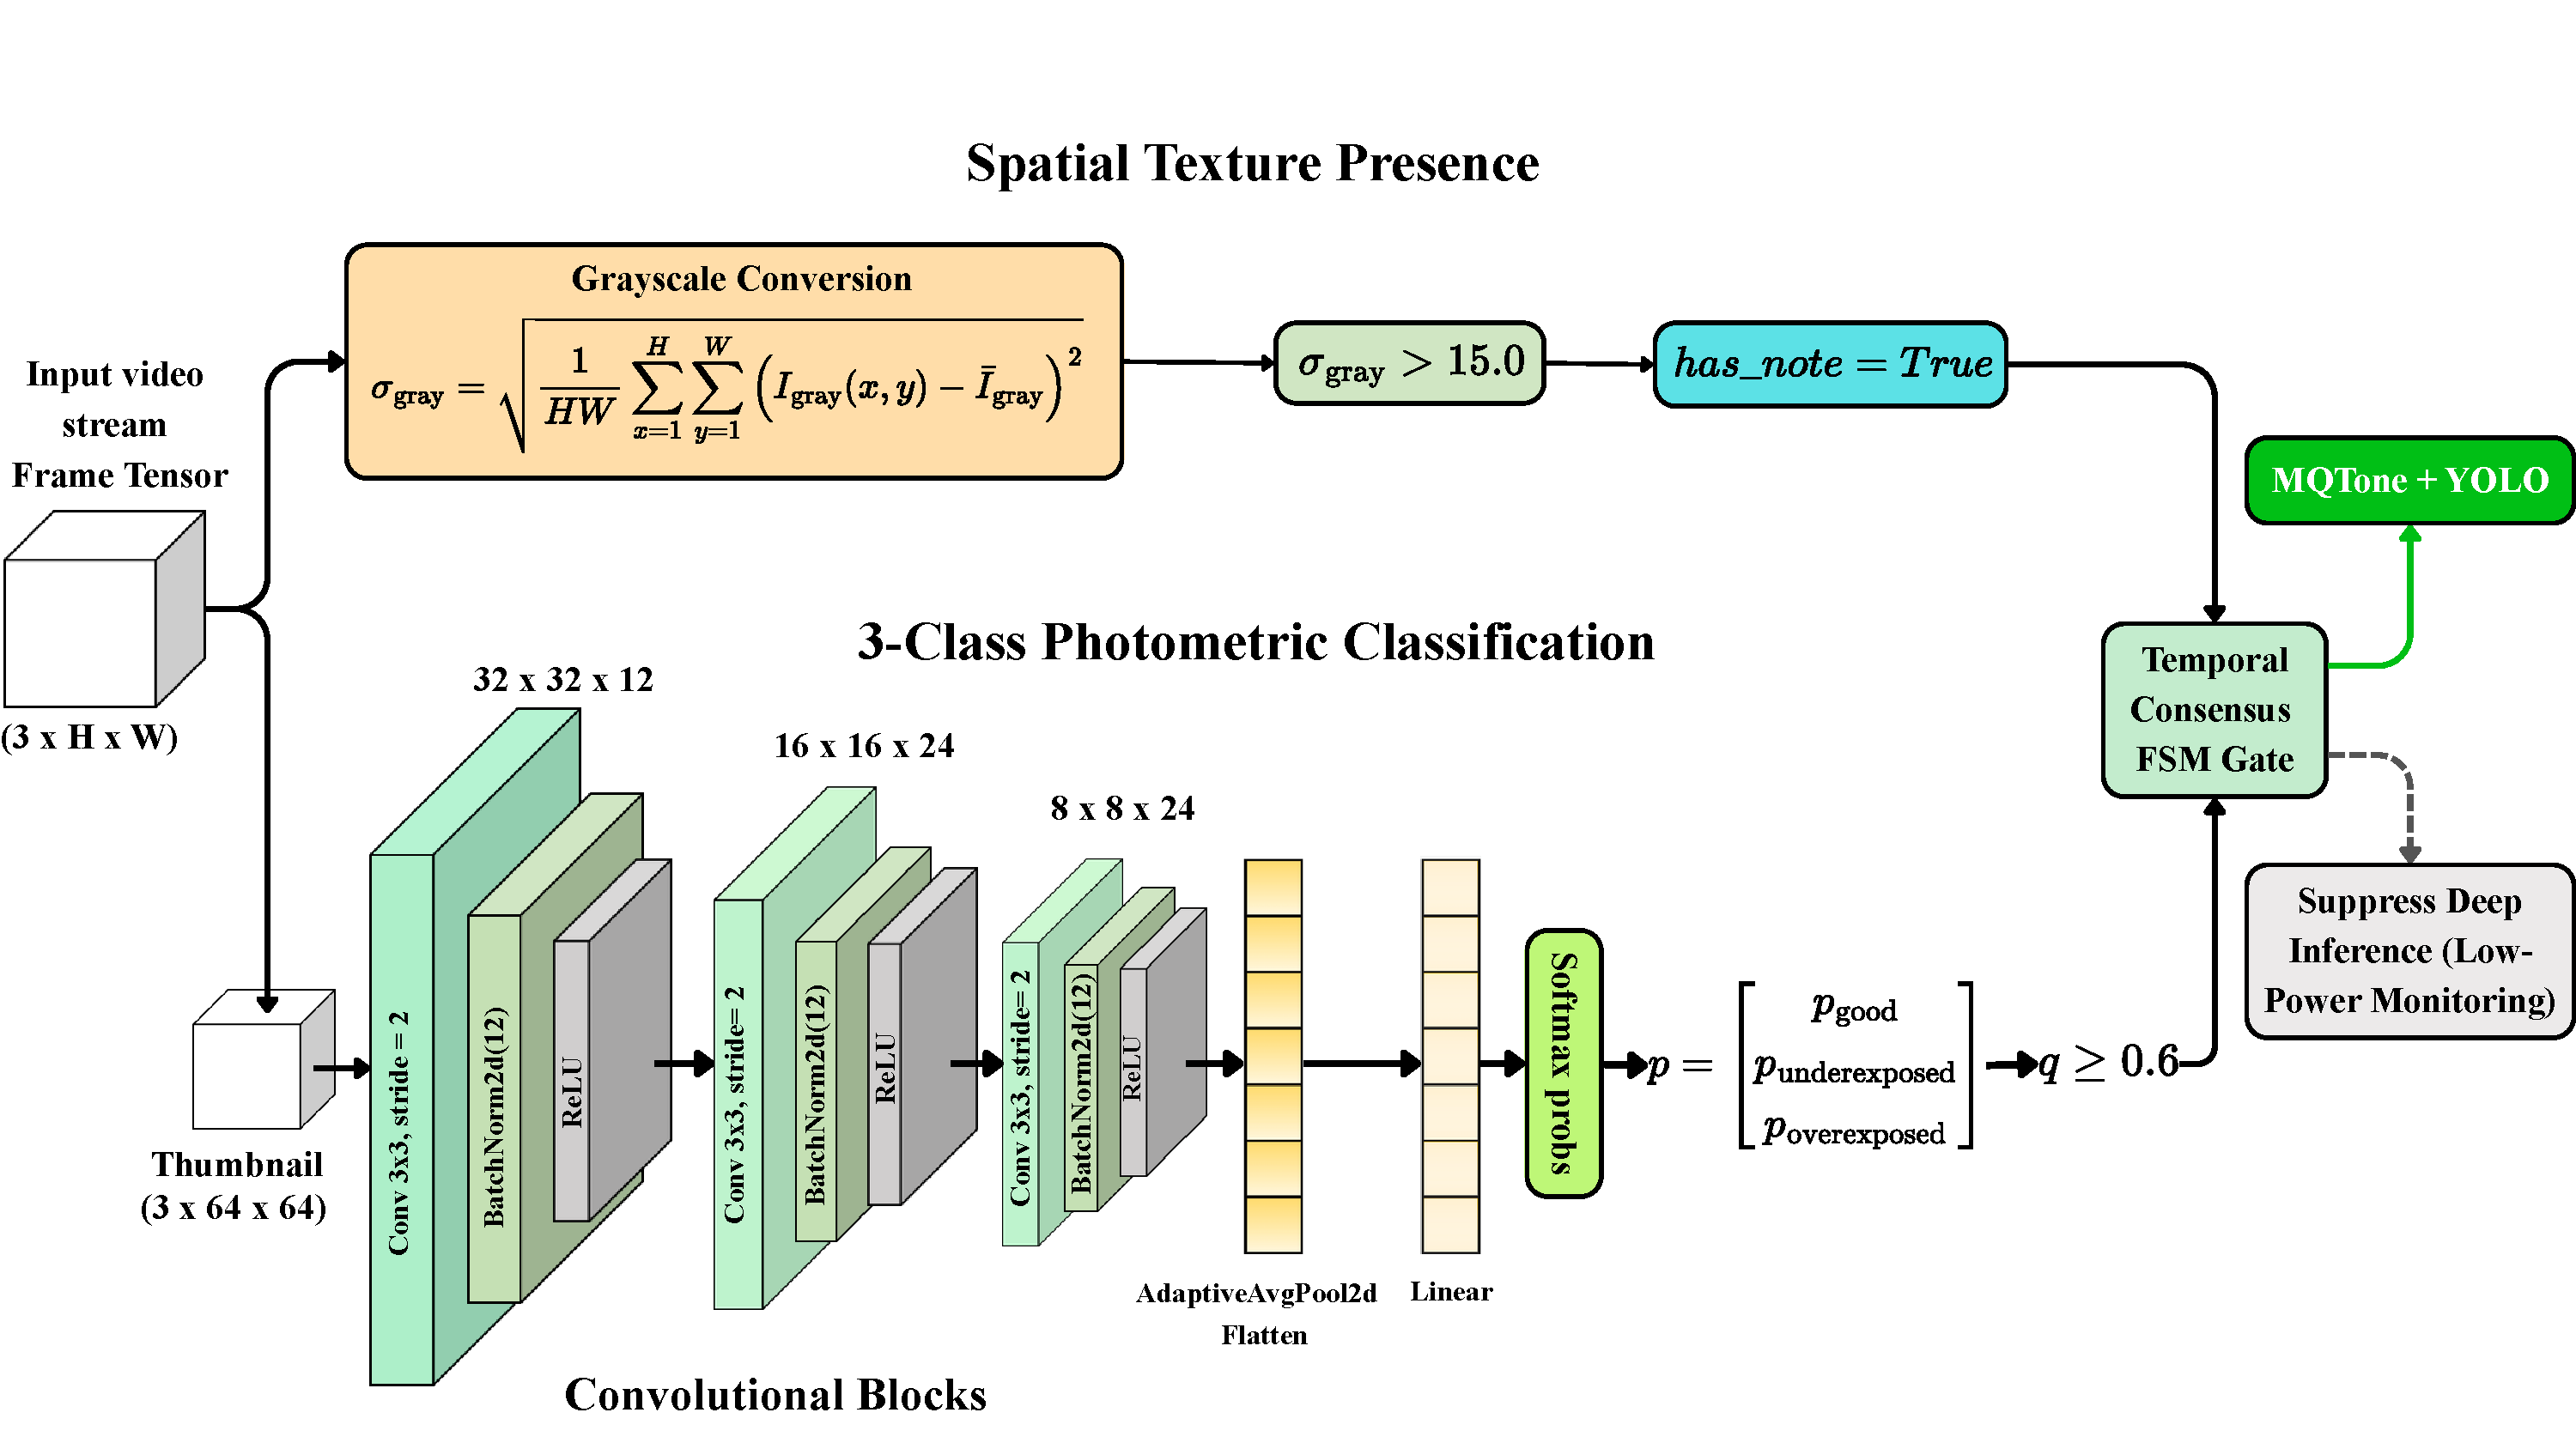
\includegraphics[width=0.92\textwidth]{lightweightopticalmodule.pdf}
\caption{Detailed architectural schematic of the proposed Lightweight Optical Monitoring Module (Quality-Gate). The module continuously inspects incoming camera buffer frames through two parallel streams: (1) an ultra-fast Spatial Texture Filter converts RGB input to perceptual luminance $I_{\text{gray}}$ via ITU-R BT.601 and evaluates the global spatial intensity standard deviation $\sigma_{\text{gray}}$ against threshold $\theta_{\text{texture}} = 15.0$ in $<0.05$\,ms to instantly filter out non-target frames (e.g., pocket occlusion, uniform tables); (2) concurrently, a bilinearly downsampled $64 \times 64 \times 3$ thumbnail is processed by a 3-stage convolutional classifier ($<50$\,KB ONNX footprint, $1.70$\,ms CPU latency) with strided convolutions, batch normalization, and adaptive global pooling to predict 3-class photometric probabilities $\mathbf{p} = [p_{\text{good}}, p_{\text{under}}, p_{\text{over}}]^\top$. The module formulates a scalar optical readiness score $q \in [0, 1]$ that sharply penalizes adverse lighting states beneath activation boundary $\tau = 0.60$. Both $\text{has\_note}$ and $q$ gate the Temporal Consensus FSM to conserve battery autonomy on mobile devices.}
\label{fig:quality_gate_architecture}
\end{figure*}

\paragraph{1. Spatial Texture Presence ($\text{has\_note}$):} Rather than executing computationally prohibitive deep neural detectors on blank, occluded, or unaligned camera frames, the system applies an ultra-fast, zero-inference spatial texture filter. This design draws upon mobile video stream-gating principles \cite{Chen2015,Zhang2017,Li2020} and lightweight embedded banknote screening \cite{Bruna2013}, which demonstrate that early rejection of uninformative frames substantially curtails mobile energy expenditure. Incoming RGB frames are first converted to a grayscale luminance channel $I_{\text{gray}} \in [0, 255]^{H \times W}$ using standard perceptual ITU-R BT.601 luminance weighting ($I_{\text{gray}} = 0.299R + 0.587G + 0.114B$) \cite{BT601,Poynton1993}. The global spatial luminance standard deviation $\sigma_{\text{gray}}$ is then evaluated as:
\begin{equation}
\sigma_{\text{gray}} = \sqrt{\frac{1}{HW} \sum_{x=1}^{H}\sum_{y=1}^{W} \left( I_{\text{gray}}(x,y) - \bar{I}_{\text{gray}} \right)^2},
\end{equation}
where $H$ and $W$ denote spatial dimensions, and $\bar{I}_{\text{gray}}$ is the mean frame luminance. Grounded in classical first-order statistical texture analysis \cite{Haralick1979,Gonzalez2008} and variance-based visual activity measurement \cite{PechPacheco2000}, $\sigma_{\text{gray}}$ quantifies the intensity dispersion and structural information entropy across the visual scene. Featureless, homogeneous environments (e.g., camera obstructed in pockets, pressed against clothing, or pointed at blank tabletop surfaces) produce negligible intensity variance ($\sigma_{\text{gray}} \le \theta_{\text{texture}}$). Conversely, polymer banknotes embossed with high-contrast portrait engravings, guilloche security patterns, transparent optical windows, and micro-lettering consistently generate substantial spatial variance ($\sigma_{\text{gray}} > \theta_{\text{texture}}$). Setting $\theta_{\text{texture}} = 15.0$ in integer pixel space $[0, 255]$ reliably filters out non-target frames, asserting $\text{has\_note} = \text{False}$ and suppressing downstream computation within $<0.05$\,ms on mobile CPUs without invoking neural inference.

\paragraph{2. 3-Class Photometric Classification:}
Concurrently, a downsampled $64 \times 64 \times 3$ thumbnail $I_{64} \in [0, 1]^{3 \times 64 \times 64}$ is processed by an ultra-compact convolutional classifier ($<50$\,KB ONNX footprint) structured as:
\begin{equation}
\label{eq:quality_cnn}
\begin{aligned}
I_{64} &\xrightarrow{\text{C}_1(s=2)} 32\times 32\times 12 \xrightarrow{\text{C}_2(s=2)} 16\times 16\times 24 \\
       &\xrightarrow{\text{C}_3(s=2)} 8\times 8\times 24 \xrightarrow{\text{Pool}} 1\times 1\times 24 \xrightarrow{\text{FC}} \mathbf{z} \in \mathbb{R}^3,
\end{aligned}
\end{equation}
where $\text{C}_k(s=2)$ is a strided $3\times 3$ convolution followed by BatchNorm and ReLU, and $\text{FC}$ is the final linear projection. The logit vector $\mathbf{z}$ is mapped via softmax to class probabilities $\mathbf{p} = [p_{\text{good}}, p_{\text{under}}, p_{\text{over}}]^\top$. An incoming frame is recognized as optically degraded when an adverse lighting class dominates with high certainty, defined by the condition $\mathbb{I}_{\text{degraded}} = \left(\arg\max(\mathbf{p}) \neq 0 \land \max(\mathbf{p}) > \tau\right)$ at calibration threshold $\tau = 0.60$. To supply a unified scalar metric for downstream temporal decision-making, the Quality-Gate computes an optical readiness score $q \in [0, 1]$:
\begin{equation}
q = \begin{cases}
p_{\text{good}}, & \text{if } \neg \mathbb{I}_{\text{degraded}}, \\
1 - \max(\mathbf{p}), & \text{if } \mathbb{I}_{\text{degraded}},
\end{cases}
\label{eq:quality_score}
\end{equation}
which preserves visual fidelity under clear illumination ($q = p_{\text{good}}$) while directly penalizing severely overexposed or underexposed captures to $q < 1 - \tau = 0.40$, safely beneath the activation boundary.

Both the spatial presence flag $\text{has\_note}$ and the scalar quality score $q$ are concurrently forwarded to the Temporal Consensus FSM (Section~\ref{subsubsec:consensus_fsm}), where together they act as an optical sensory gatekeeper: whenever $\text{has\_note} = \text{False}$ or $q < \tau$, deep neural inference is suppressed, preserving battery autonomy on unaligned or poorly illuminated frames until sustained optical stability is verified. While severe kinetic motion blur causes contrast smearing that depresses $p_{\text{good}} < \tau$, physical geometric misalignments (such as out-of-plane banknote tilts $>65^\circ$ or heavy hand occlusions $>50\%$) that clear optical gating are handled downstream by YOLOv8n confidence filtering ($\text{conf} < \theta_{\text{conf}}$), safely deferring unidentifiable presentations without false alarms.

\subsubsection{MQTone: Spatially Adaptive Tone-Mapping Sub-network}
\label{subsubsec:mqtone}
Polymer banknotes manufactured from BOPP feature non-porous specular substrates, clear security windows, and metallic diffractive gratings. Under ambient sunlight or directional artificial luminaires, these surfaces produce severe localized overexposure and specular highlight blowout that saturate camera sensors and obscure fine denomination numerals. Existing lightweight enhancers (e.g., Zero-DCE++ \cite{Li2021}, IAT \cite{Cui2022}) apply monotonic low-light brightening curves, which amplify specular blowout on reflective polymer surfaces and obscure subtle security engravings.

To solve this, we propose \textbf{MQTone} (Micro-scale Quality Tone-mapping Network), an ultra-lightweight ($19{,}686$ parameters, $<0.1$\,MB footprint, $23.2$\,ms on mobile CPU) dual-branch sub-network that jointly estimates global photometric parameters and localized spatial residual maps (detailed structurally in Figure~\ref{fig:mqtone_architecture}). Rather than performing pixel-to-pixel synthesis at full resolution, MQTone predicts a compact parameter grid on a $64 \times 64$ thumbnail and projects it onto the full-resolution input $I \in [0, 1]^{3 \times H \times W}$ via bilinear interpolation.

\begin{figure*}[t]
\centering
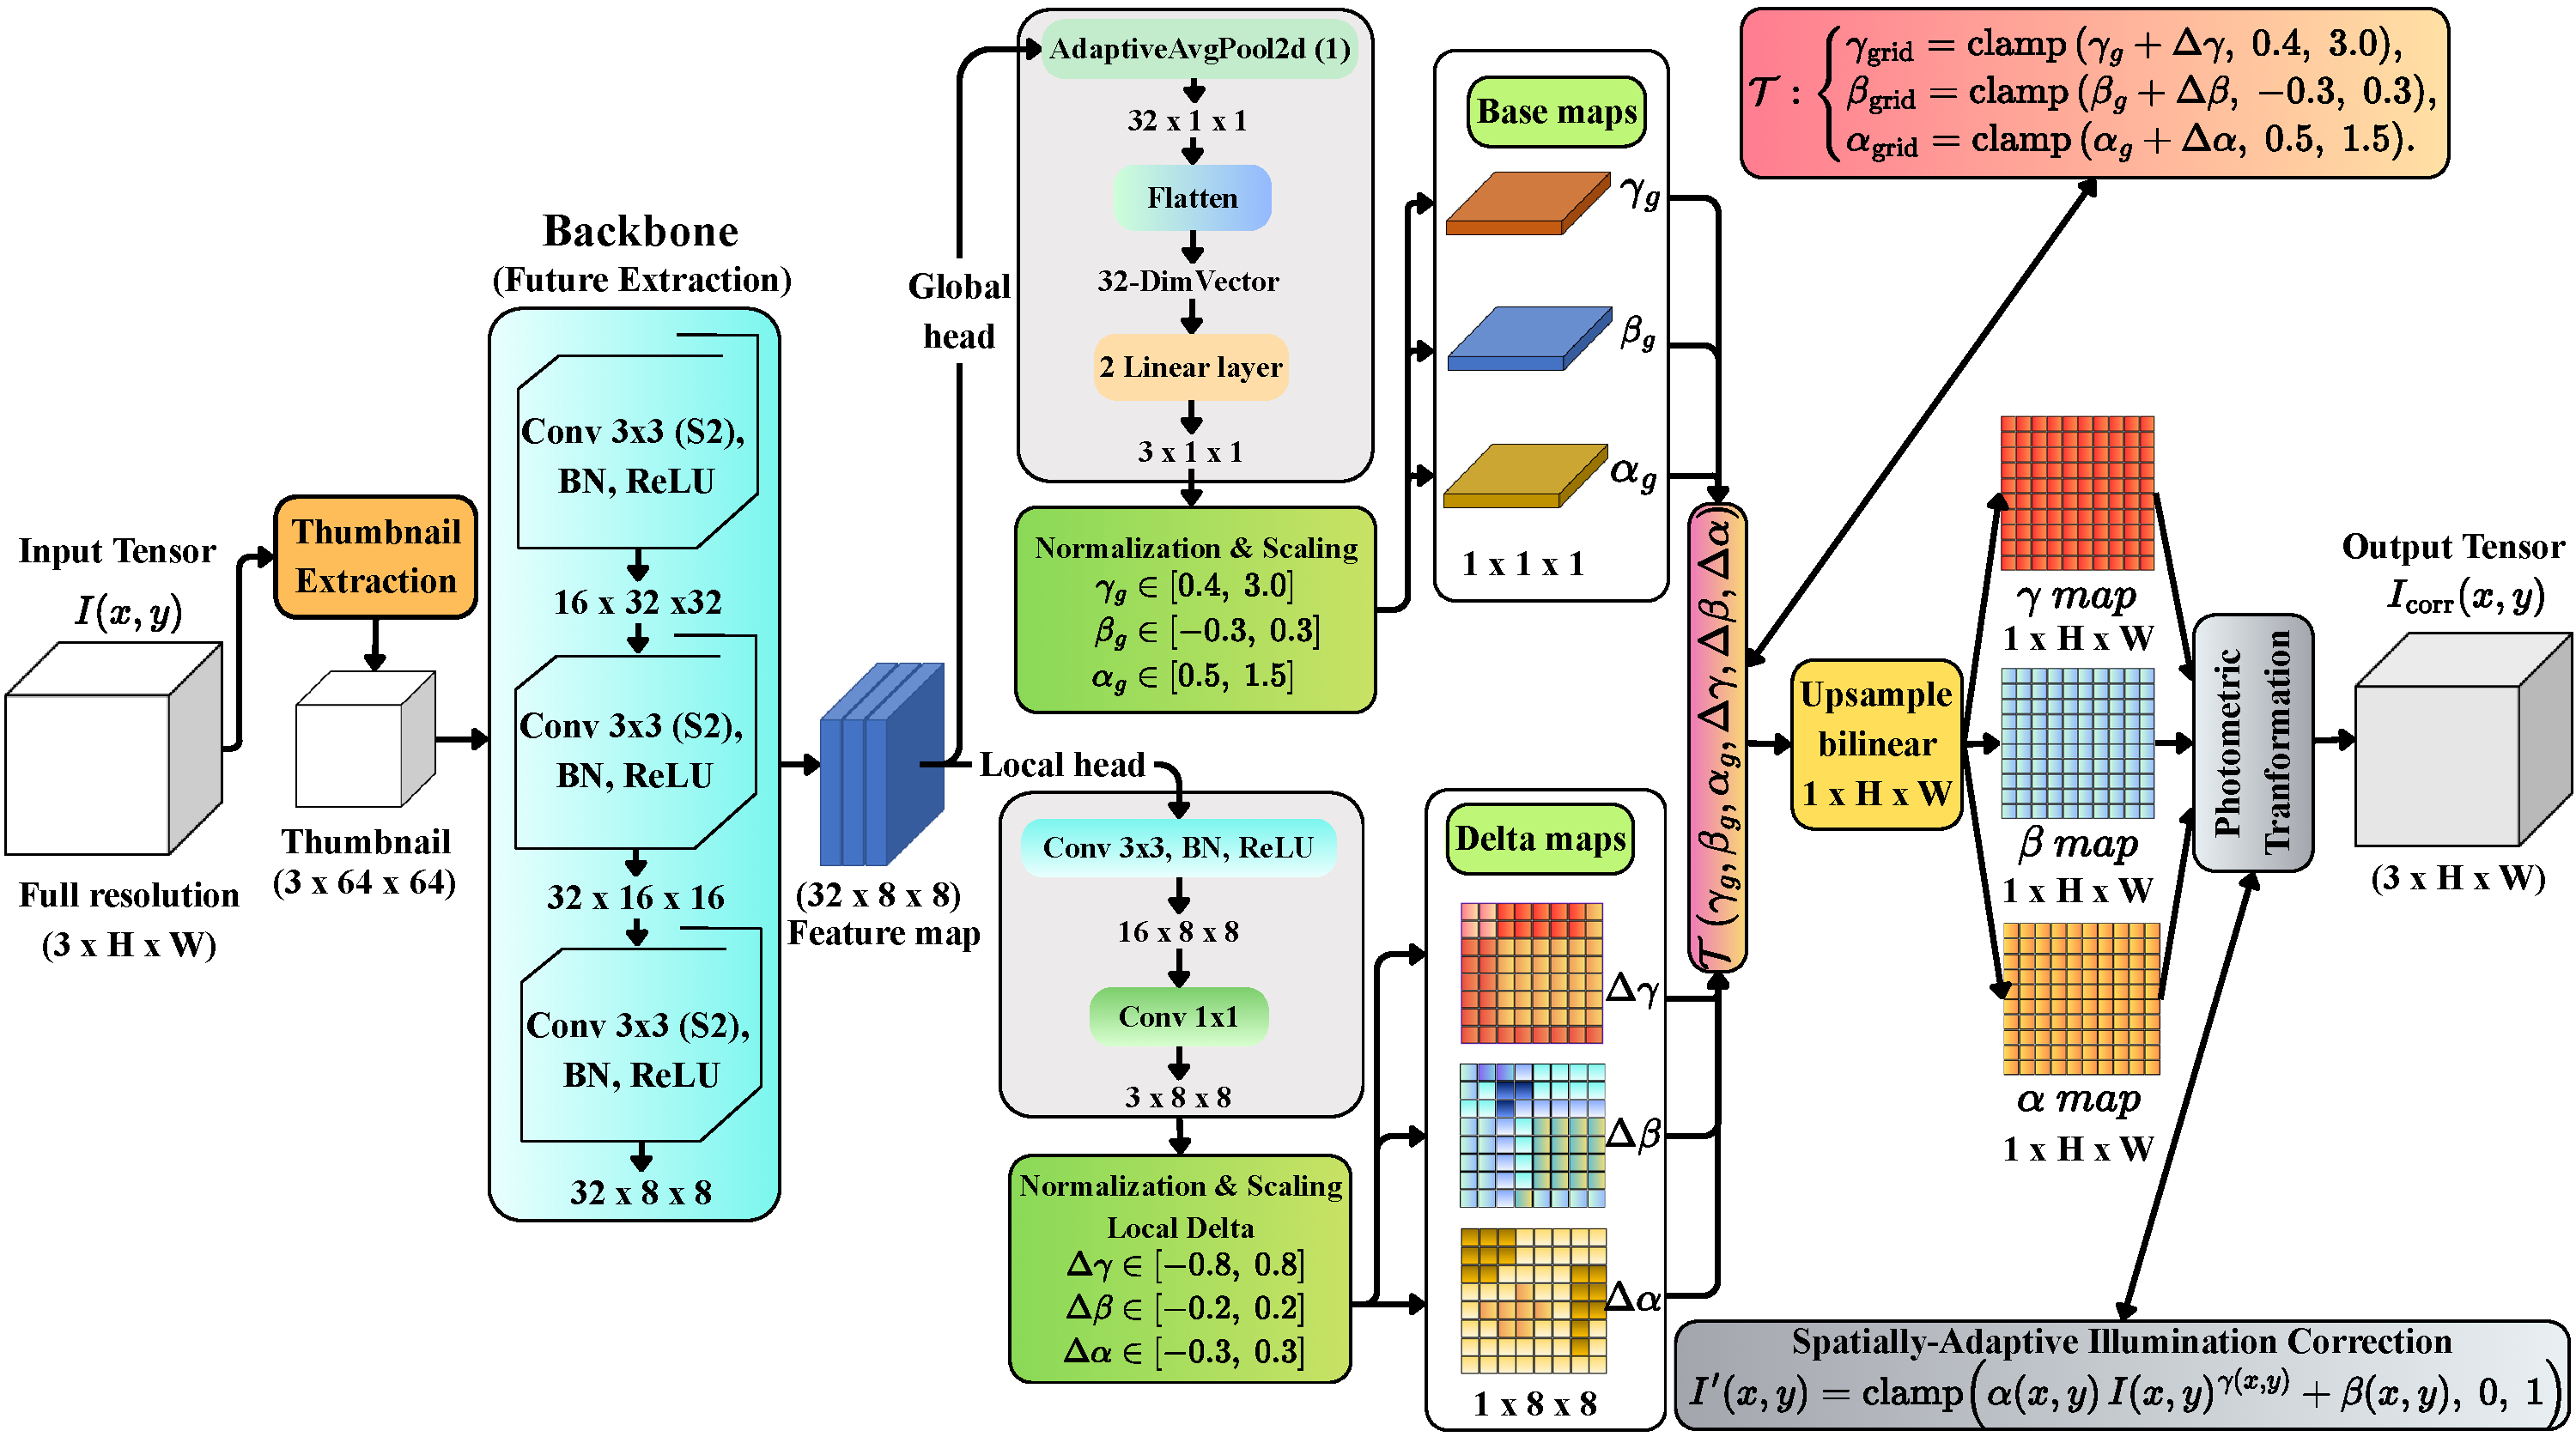
\includegraphics[width=0.92\textwidth]{mqtone.pdf}
\caption{Detailed architectural schematic of the proposed MQTone (Micro-scale Quality Tone-mapping Network) sub-network. Operating on a lightweight $64 \times 64$ thumbnail, a shared convolutional backbone extracts an $8 \times 8 \times 32$ feature representation. Two parallel prediction heads decouple illumination correction: (1) the Global Parameter Head estimates base curve coefficients $(\gamma_g, \beta_g, \alpha_g)$, while (2) the Local $8 \times 8$ Grid Head predicts spatial residual maps $(\Delta\gamma, \Delta\beta, \Delta\alpha)$ to selectively suppress localized specular glare and recover obscured tactile textures without darkening unshaded regions. The combined parameters are smoothly upsampled via bilinear interpolation to full camera resolution ($H \times W$) for artifact-free, pixel-wise photometric transformation.}
\label{fig:mqtone_architecture}
\end{figure*}

\paragraph{Architecture and Parameter Prediction:}
A shared convolutional backbone maps $I_{64}$ to an intermediate feature map $\mathbf{F} \in \mathbb{R}^{32 \times 8 \times 8}$ through three strided convolutional stages ($3 \to 16 \to 32 \to 32$ channels with batch normalization and ReLU activations). From $\mathbf{F}$, two specialized heads operate in parallel:
\begin{itemize}
    \item \textbf{Global Parameter Head:} Features are pooled globally via $\text{AdaptiveAvgPool2d}(1)$ and projected through two fully-connected layers ($32 \to 16 \to 3$) to estimate base photometric coefficients $\mathbf{g}_{\text{raw}} \in \mathbb{R}^3$. These are bounded via activation functions to safe operational ranges:
    \begin{align}
    \gamma_g &= 0.4 + 2.6 \cdot \sigma(g_{\text{raw}, 0}) \in [0.4, 3.0], \\
    \beta_g  &= 0.3 \cdot \tanh(g_{\text{raw}, 1}) \in [-0.3, 0.3], \\
    \alpha_g &= 0.5 + 1.0 \cdot \sigma(g_{\text{raw}, 2}) \in [0.5, 1.5],
    \end{align}
    where $\sigma(\cdot)$ denotes the standard sigmoid function.
    \item \textbf{Local $8 \times 8$ Grid Head:} To compensate for non-uniform specular highlights and localized shadows across the polymer substrate, a compact convolutional head ($\text{Conv } 3\times 3, 32 \to 16 \to \text{BN, ReLU} \to \text{Conv } 1\times 1, 16 \to 3$) estimates an $8 \times 8$ spatial residual tensor $\mathbf{L}_{\text{raw}} \in \mathbb{R}^{3 \times 8 \times 8}$:
    \begin{align}
    \Delta\gamma(u,v) &= 0.8 \cdot \tanh(L_{\text{raw}, 0}(u,v)) \in [-0.8, 0.8], \\
    \Delta\beta(u,v)  &= 0.2 \cdot \tanh(L_{\text{raw}, 1}(u,v)) \in [-0.2, 0.2], \\
    \Delta\alpha(u,v) &= 0.3 \cdot \tanh(L_{\text{raw}, 2}(u,v)) \in [-0.3, 0.3],
    \end{align}
    for grid spatial coordinates $u, v \in \{1, \dots, 8\}$.
\end{itemize}
The global coefficients and local residuals are summed and clamped to form an $8 \times 8$ parameter grid:
\begin{align}
\gamma_{\text{grid}} &= \text{clip}\left(\gamma_g + \Delta\gamma,\, 0.4,\, 3.0\right), \\
\beta_{\text{grid}}  &= \text{clip}\left(\beta_g + \Delta\beta,\, -0.3,\, 0.3\right), \\
\alpha_{\text{grid}} &= \text{clip}\left(\alpha_g + \Delta\alpha,\, 0.5,\, 1.5\right).
\end{align}

\paragraph{Bilinear Upsampling and Photometric Transform:}
To ensure smooth spatial transitions across the full camera resolution without blocking artifacts, the grid parameters are upsampled via bilinear interpolation $\mathcal{U}_{\text{bilinear}}$ to dimensions $H \times W$:
\begin{equation}
(\gamma, \beta, \alpha) = \mathcal{U}_{\text{bilinear}}\left( \gamma_{\text{grid}},\, \beta_{\text{grid}},\, \alpha_{\text{grid}} \right).
\end{equation}
The corrected image $I_{\text{corr}} \in [0, 1]^{3 \times H \times W}$ is then generated through pixel-wise non-linear remapping:
\begin{equation}
I_{\text{corr}}(x,y) = \text{clip}\left( \alpha(x,y) I(x,y)^{\gamma(x,y)} + \beta(x,y),\, 0,\, 1 \right).
\label{eq:mqtone_transform}
\end{equation}

\paragraph{Identity Weight Initialization and Joint Loss:}
To prevent gradient divergence and destabilization during early training epochs, MQTone incorporates identity-preserving initialization: the bias of the final linear layer in the global head is explicitly set to $b_{\gamma} = \ln((1.0 - 0.4)/(3.0 - 1.0))$, $b_{\beta} = 0.0$, and $b_{\alpha} = 0.0$, while the local head weights are initialized with a near-zero standard deviation ($\sigma = 10^{-3}$). As a result, at epoch 0, $\gamma(x,y) \equiv 1.0$, $\beta(x,y) \equiv 0.0$, and $\alpha(x,y) \equiv 1.0$, ensuring that MQTone begins training from an identity transformation $I_{\text{corr}} \equiv I$.

MQTone is jointly supervised alongside the detector using a compound loss function:
\begin{equation}
\mathcal{L}_{\text{total}} = \mathcal{L}_{\text{det}} + \lambda_{\text{photo}} \mathcal{L}_{\text{photo}},
\label{eq:total_loss}
\end{equation}
where $\mathcal{L}_{\text{det}}$ is the multi-task YOLO detection loss, and $\mathcal{L}_{\text{photo}} = \| I_{\text{corr}} - I_{\text{clean}} \|_1$ enforces direct $\ell_1$ photometric alignment between degraded inputs and paired clean reference frames, set with $\lambda_{\text{photo}} = 1.0$.

\subsubsection{Joint Defect Detection and Temporal Consensus FSM}
\label{subsubsec:consensus_fsm}

\begin{figure*}[t]
\centering
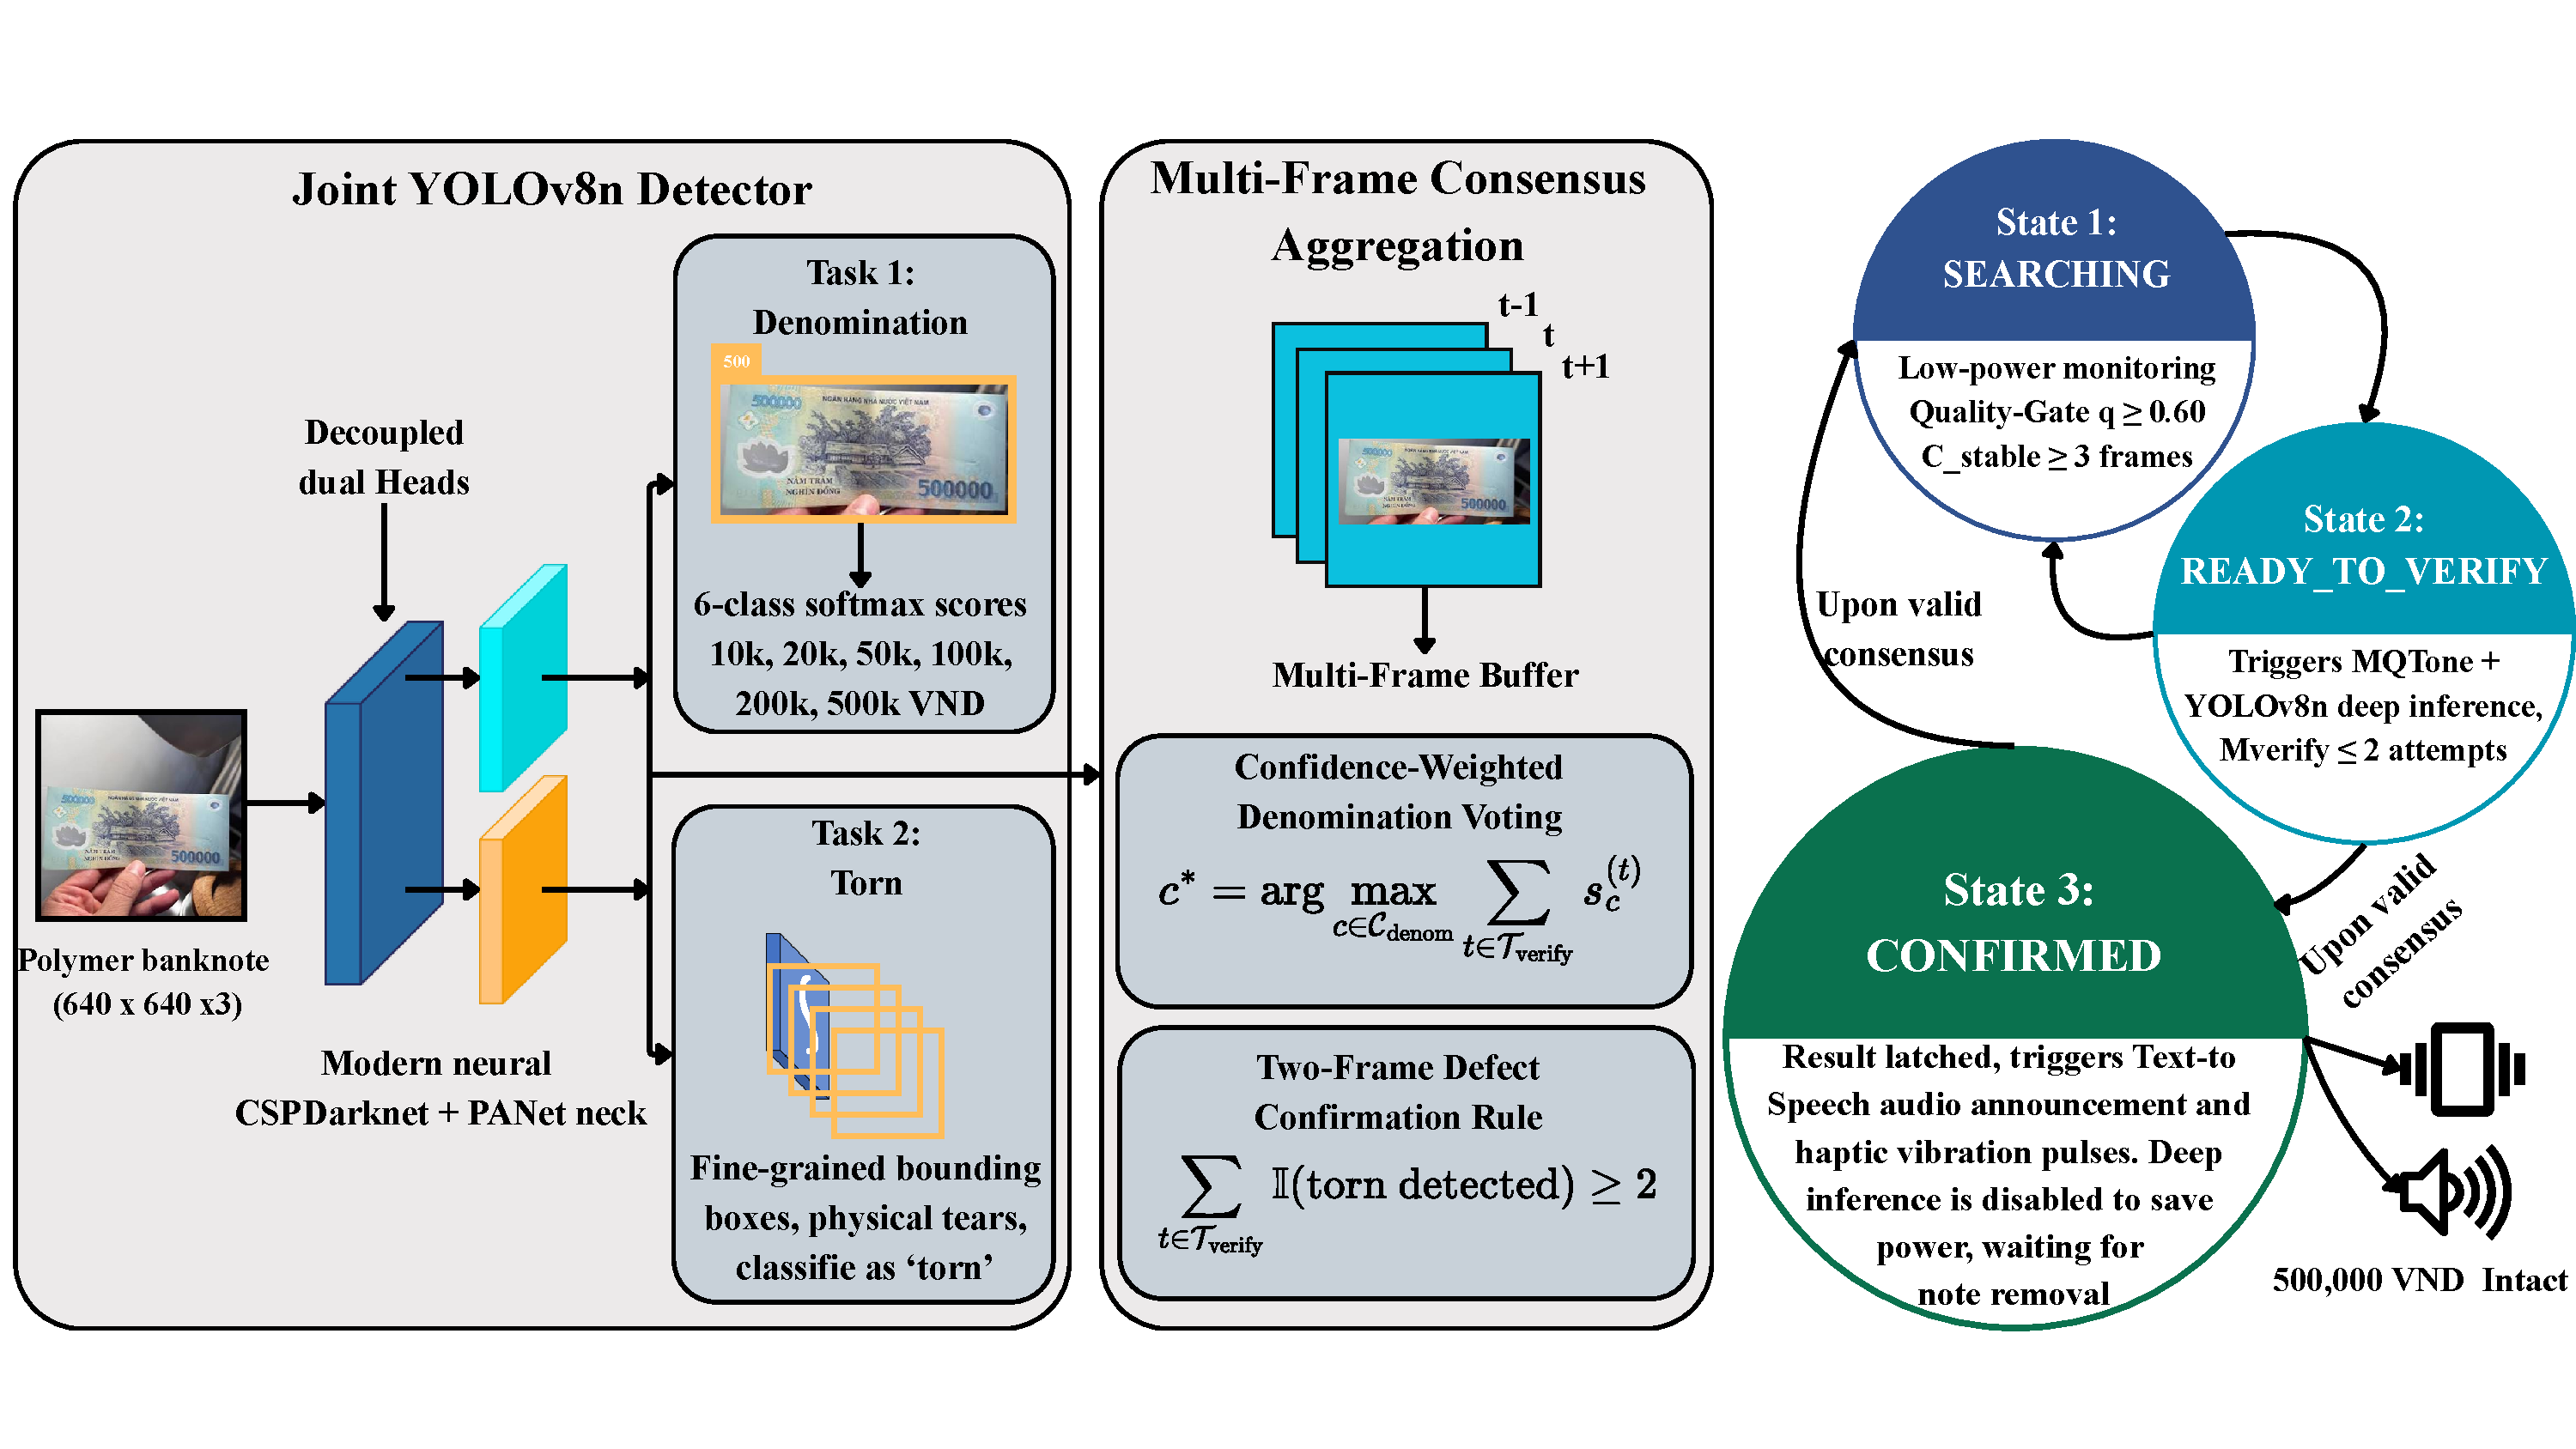
\includegraphics[width=0.92\textwidth]{joint.pdf}
\caption{Detailed architectural schematic of the downstream Joint Defect-Denomination YOLOv8n Detector and the 3-State Temporal Consensus Finite State Machine (FSM). Left: Decoupled dual-head detector operating on enhanced frames ($640 \times 640 \times 3$) to concurrently predict 6-class currency denomination (Task 1) and localize physical substrate fractures (Task 2, class \texttt{torn}). Right: Three-state temporal consensus FSM (\texttt{SEARCHING}, \texttt{READY\_TO\_VERIFY}, and \texttt{CONFIRMED}) integrating multi-frame buffer aggregation, confidence-weighted denomination voting, and two-frame defect latching to mitigate acoustic fluttering while suppressing redundant deep neural invocations once confirmed.}
\label{fig:joint_consensus_fsm}
\end{figure*}

\paragraph{Joint Defect-Denomination YOLOv8n Detector:}
As illustrated in Fig.~\ref{fig:joint_consensus_fsm} (left), downstream currency inspection is performed by an anchor-free YOLOv8n detector ($12.3$\,MB ONNX footprint, $3.2$\,M parameters) operating at $640 \times 640$ input resolution. The network utilizes a modified CSPDarknet backbone with Path Aggregation Network (PANet) neck and decoupled detection heads (separating classification and bounding-box regression branches across P3--P5 feature maps). Rather than maintaining fragmented models, the detector executes joint dual-task multi-class inference over seven semantic categories (six circulating polymer denominations and one substrate fracture class \texttt{torn}):
\begin{enumerate}[label=(\roman*)]
    \item \textbf{Denomination Identification Task:} Predicts currency denomination $c \in \{10\text{k},\allowbreak 20\text{k},\allowbreak 50\text{k},\allowbreak 100\text{k},\allowbreak 200\text{k},\allowbreak 500\text{k}\}$ and full banknote bounding box coordinates $\mathbf{b}_{\text{note}} \in \mathbb{R}^4$ via class score maximization across the denomination indices.
    \item \textbf{Defect Localization Task:} Concurrently localizes bounding boxes $\mathbf{b}_{\text{torn}} \in \mathbb{R}^4$ for physical substrate fractures (class \texttt{torn}), distinguishing pristine notes from damaged currency requiring financial caution.
\end{enumerate}
The multi-task detection objective is optimized end-to-end via:
\begin{equation}
\mathcal{L}_{\text{det}} = \lambda_{\text{cls}} \mathcal{L}_{\text{BCE}} + \lambda_{\text{box}} \mathcal{L}_{\text{CIoU}} + \lambda_{\text{dfl}} \mathcal{L}_{\text{DFL}},
\end{equation}
combining Task-Aligned Binary Cross-Entropy Loss ($\mathcal{L}_{\text{BCE}}$) for multi-class classification, Complete IoU Loss ($\mathcal{L}_{\text{CIoU}}$) for bounding box regression, and Distribution Focal Loss ($\mathcal{L}_{\text{DFL}}$) for sub-pixel boundary representation.

\paragraph{Temporal Consensus Finite State Machine (FSM):}
Under unconstrained mobile handling, hand tremor, perspective jitter, and momentary glare routinely corrupt individual video frames. Relying on unverified single-frame inferences exposes assistive users to acoustic fluttering and financial misclassifications.

To achieve reliable and jitter-free acoustic guidance, CashVision integrates a 3-state Temporal Consensus FSM (Fig.~\ref{fig:joint_consensus_fsm}, right) functioning as the runtime inference engine that executes the declarative Knowledge Base (Table~\ref{tab:expert_rule_base}):
\begin{itemize}
    \item \textbf{State 1: $\texttt{SEARCHING}$.} The system runs exclusively in low-power sensory monitoring mode via the Quality-Gate. A pre-inference stability counter $c_{\text{stable}}$ tracks consecutive incoming frames satisfying both Rule $R_1$ (spatial texture gating, $\sigma_{\text{gray}} > \theta_{\text{texture}} = 15.0$) and Rule $R_2$ (photometric quality acceptance, $q \ge \tau = 0.60$). In accordance with Rule $R_3$, when $c_{\text{stable}} \ge K_{\text{opt}} = 3$ consecutive stable frames, the inference engine transitions to $\texttt{READY\_TO\_VERIFY}$. If the note leaves the view ($\sigma_{\text{gray}} \le \theta_{\text{texture}}$) or optical quality degrades ($q < \tau$), $c_{\text{stable}}$ immediately resets to 0.
    \item \textbf{State 2: $\texttt{READY\_TO\_VERIFY}$.} Governed by Meta-Level Control, the full inspection pipeline (MQTone + YOLOv8n) is triggered across a burst verification window bounded by Rule $R_4$ ($M_{\text{verify}} = 2$ attempts). Candidate bounding boxes are filtered via Rule $R_5$ ($\text{conf} \ge \theta_{\text{conf}} = 0.25$, the established post-NMS default threshold in Ultralytics YOLO architectures \cite{Jocher2023}) and submitted to multi-frame temporal consensus (Rules $R_6$ and $R_7$, detailed below). If consensus is reached, the inference engine transitions to $\texttt{CONFIRMED}$. If detection or consensus fails after $M_{\text{verify}}$ attempts, the FSM safely transitions back to $\texttt{SEARCHING}$, preventing continuous compute-bound execution and thermal throttling.
    \item \textbf{State 3: $\texttt{CONFIRMED}$.} Upon transition, the \textit{Explanation Facility} is activated: the confirmed denomination and defect status are latched and synthesized into natural speech via Android Text-to-Speech (TTS) alongside differentiated haptic vibration cues (single pulse for intact notes, dual pulses for detected tears), providing immediate, transparent feedback to the visually impaired operator. Once in $\texttt{CONFIRMED}$, Meta-Level Control suppresses further deep neural inferences, dropping per-frame compute back to the lightweight $1.7$\,ms Quality-Gate monitoring while holding the verified result in memory.
    
    To prevent the system from remaining indefinitely locked in $\texttt{CONFIRMED}$ when placed on high-contrast textured backgrounds (e.g., wooden desks, patterned tablecloths, or user hands where $\sigma_{\text{gray}}$ remains $> 15.0$), the FSM incorporates the dual-condition reset criteria defined in Rule $R_8$: the system resets back to $\texttt{SEARCHING}$ when either:
    \begin{enumerate}[label=(\alph*)]
        \item Global spatial luminance standard deviation drops below threshold ($\sigma_{\text{gray}} \le \theta_{\text{texture}} = 15.0$, Rule $R_{8\text{a}}$), indicating note removal into a featureless background or pocket; OR
        \item A dynamic scene-transition or banknote-withdrawal event is detected via temporal mean luminance shift ($|\bar{I}_t - \bar{I}_{\text{latched}}| > \theta_{\text{trans}} = 25.0$, Rule $R_{8\text{b}}$) or the absence of a confirmed banknote contour across a lightweight periodic verification check executed every $1.5$\,s.
    \end{enumerate}
\end{itemize}

\paragraph{Multi-Frame Consensus Aggregation:}
To mitigate acoustic fluttering and reduce false alarms caused by transient specular flashes or hand tremor across verification candidates, CashVision incorporates multi-frame temporal consensus rules across triggered verification frames $\mathcal{T}_{\text{verify}}$:
\begin{enumerate}[label=(\alph*)]
    \item \textbf{Confidence-Weighted Denomination Voting (Rule $R_6$):} Candidate detections across the verification window are aggregated via confidence score summation:
    \begin{equation}
    c^* = \arg\max_{c \in \mathcal{C}_{\text{denom}}} \sum_{t \in \mathcal{T}_{\text{verify}}} s_c^{(t)},
    \end{equation}
    where $s_c^{(t)}$ denotes the predicted confidence for denomination class $c$ at frame $t$. This voting scheme ensures that consistent, high-certainty predictions consistently prevail over transient boundary misclassifications.
    \item \textbf{Two-Frame Defect Confirmation Rule (Rule $R_7$):} Physical substrate fractures (class \texttt{torn}) are confirmed if and only if tear detections persist across at least two triggered verification frames ($\sum_{t \in \mathcal{T}_{\text{verify}}} \mathbb{I}(\text{torn detected}) \ge 2$). While specular reflection spots or sharp creases can momentarily produce isolated edge artifacts on a single frame, genuine structural tears consistently persist across consecutive viewpoints, thereby suppressing false-positive damage alerts.
\end{enumerate}

\paragraph{On-Device Embedded Stack and Deployed Checkpoint:}
The deep models (Quality-Gate, MQTone, and YOLOv8n) are deployed using the native ONNX Runtime mobile C++ inference engine with intra-op multi-threaded CPU execution (2 threads) on Android, orchestrated by the Meta-Level Control layer. The model deployed to the smartphone corresponds to the Fold-1 checkpoint from Protocol~B (which attained median cross-validation accuracy on the hybrid validation set). All image pre-processing, state transitions, and neural inferences run $100\%$ offline on the device without network connectivity, ensuring user privacy, zero cloud latency, and dependable assistive autonomy in network-deprived environments.

% Experimental results will be elaborated here.
\section{Experimental Results}
\label{sec:experiments}
\subsection{Experimental Setup and Data Partitioning Protocols}
\label{subsec:exp_setup}

The static benchmark comprises $1{,}812$ annotated polymer banknote images ($302$ images per denomination across six circulating values: 10k, 20k, 50k, 100k, 200k, and 500k VND) span across six operational conditions: standard indoor ($390$), outdoor daylight ($390$), strong backlighting ($306$), severe specular overexposure ($306$), clean physical tears ($210$), and glare-degraded tears ($210$). To systematically evaluate cross-condition degradation and photometric robustness across adverse environments without data contamination, we establish two empirical experimental protocols.

\paragraph{Protocol A: Baseline Cross-Condition Degradation and Domain Shift}
To investigate how conventional banknote inspection models trained under normal, non-adverse everyday lighting conditions behave when exposed to unconstrained, adverse real-world environments, we establish a closed-to-open stress-test protocol using all $1{,}812$ annotated images without synthetic enhancement. The training pool is restricted to authentic captures under normal, favorable real-world ambient illumination (non-adverse everyday lighting), comprising $600$ images ($390$ pristine $\texttt{indoor}$ bills under standard ambient lighting and $210$ $\texttt{torn\_clean}$ bills without harsh reflections). A 5-fold stratified cross-validation split (stratified by joint denomination class and physical defect state) is executed within this pool. Each fold allocates $480$ images ($80\%$, comprising $312$ indoor and $168$ torn-clean samples) for training and $120$ images ($20\%$, comprising $78$ indoor and $42$ torn-clean samples) for in-distribution baseline validation.

Because each denomination is represented by multiple continuous photoshoot frames of the physical specimens, random frame-level partitioning within this benign pool allows physical specimens to be shared across training and in-distribution validation splits (accounting for the high $99.67\%$--$100.0\%$ baseline ceiling). This design isolates cross-condition degradation: Protocol~A's purpose is to establish an in-distribution upper-bound reference and evaluate how models trained under favorable indoor conditions degrade when exposed to out-of-distribution (OOD) adverse environments ($1{,}212$ images: $390$ $\texttt{outdoor}$, $306$ $\texttt{backlight}$, $306$ $\texttt{overexposed}$, and $210$ $\texttt{torn\_bright}$) without fine-tuning, reflecting environmental domain shift under shared physical notes rather than generalization to unseen physical banknotes.

\paragraph{Protocol B: Cross-Condition Photometric Invariance via Synthetic Optical Degradation:}
To establish whether MQTone can learn robust photometric invariance without requiring real-world adverse training samples, Protocol B evaluates cross-condition illumination robustness from benign indoor lighting to challenging real-world environments on the 1,812-image static benchmark. The training pool is isolated to $420$ diffuse indoor captures ($270$ pristine and $150$ clean-torn notes) drawn from the canonical training partition. The remaining held-out evaluation captures are partitioned into two quarantined subsets: $126$ real adverse images serve as a Generalization Development Set dedicated to cross-condition validation checkpoint selection and hyperparameter calibration ($\theta_{\text{texture}} = 15.0$, $\tau = 0.60$, $K_{\text{opt}} = 3$, $M_{\text{verify}} = 2$), while the remaining $1{,}266$ multi-condition images (formed by merging the $714$ remaining adverse images from the training partition with the $552$ canonical validation and test images, spanning all six operational conditions) form the Locked Holdout Evaluation Benchmark for final testing ($420 + 126 + 1{,}266 = 1{,}812$). This locked benchmark evaluates cross-illumination and cross-condition performance across real adverse captures. Because the dataset was acquired across continuous photoshoot sessions per denomination, the $552$ merged canonical validation and test images share physical banknote specimens with the training pool; likewise, the $\texttt{torn\_clean}$ and $\texttt{torn\_bright}$ subsets evaluate identical physical banknotes under neutral versus specular illumination. Protocol~B therefore measures photometric and environmental invariance across glare, backlighting, and tear defects, rather than generalization to unseen physical banknote specimens. Specimen-disjoint generalization---where physical banknotes are partitioned to prevent note-level leakage---is formulated in Section~\ref{subsec:specimen_disjoint_results} under a dedicated Leave-Specimen-Out evaluation protocol. This operational constraint explains why baseline recognition accuracy settles at an authentic ceiling ($86.50\%$ baseline denomination accuracy vs.\ $99.67\%$ in Protocol~A).

Within the 420-image pool, 5-fold stratified cross-validation allocates $336$ raw images for training and $84$ raw images for validation per fold. To expose MQTone to the physical reflectance properties of polymer BOPP substrates without exposing it to real-world test scenes, an optical degradation augmentation pipeline synthetically generates localized polymer-specific artifacts:
\begin{enumerate}[label=(\roman*)]
    \item \textbf{Specular Glare Synthesis:} Elliptical masks smoothed via Gaussian filtering ($k \ge 15$) with additive intensity boosts ($+70$ to $+160$ pixel levels) synthesize localized specular flash reflections.
    \item \textbf{Directional and Local Occlusions:} Elliptical luminance reduction ($35\%$--$65\%$) and edge-oriented linear gradient ramps simulate user finger shadowing and non-uniform backlighting.
    \item \textbf{Photometric Pair Synthesis:} Overexposure ($\Delta\text{brightness} \in [+0.20, +0.35]$, $\gamma \in [0.60, 0.85]$) and underexposure ($\Delta\text{brightness} \in [-0.35, -0.20]$, $\gamma \in [1.15, 1.50]$) mappings simulate extreme sensor saturation.
    \item \textbf{Structural Defect Balancing:} Oversampling damaged substrate instances ($\texttt{torn}$ class) ensures equitable representation against pristine banknotes.
\end{enumerate}
Through this synthesis, each raw image generates five base instances (one original plus four synthetic variations: photometric, light-pair, dark-pair, and local-only). The remaining instances arise from structural defect balancing on the torn notes: in training, the $120$ torn notes receive $3$ additional oversampled copies per note ($336 \times 5 + 120 \times 3 = \mathbf{2{,}040}$ instances); in validation, the $30$ torn notes receive $5$ copies per note ($84 \times 5 + 30 \times 5 = \mathbf{570}$ instances) to achieve target defect representation despite smaller sample size. Each fold's validation set comprises $\mathbf{696}$ images in total, formed by combining the fold's $570$ synthetically augmented validation frames with the Generalization Development Set. This hybrid validation scheme ensures that checkpoint selection is guided by cross-condition robustness rather than overfitting to synthetic augmentation artifacts alone. Every synthetically degraded training instance maintains a reference pointer ($\texttt{orig\_img\_path}$) to its pristine clean progenitor to optimize the reconstruction loss $\mathcal{L}_{\text{photo}} = \| I_{\text{corr}} - I_{\text{clean}} \|_1$. All candidate models evaluated under Protocol~B---including the Baseline (augmented training, no enhancer), classical heuristics (Gamma, CLAHE), and all deep architectures---are trained identically on the same $2{,}040$-image augmented training pool, so the Baseline (augmented training, no enhancer) functions as an explicit ablative benchmark that isolates the effect of synthetic data augmentation alone, allowing direct quantification of the incremental gain provided by the active MQTone tone-mapping module. Finally, the models selected on each fold are evaluated directly against the $1{,}266$-image locked multi-condition benchmark.

\paragraph{Quality-Gate Module Training and Dual-Tier Screening:}
The Quality-Gate is constructed as an ultra-lightweight sensory classifier ($<50$\,KB ONNX footprint, $1.70 \pm 0.04$\,ms CPU latency) processing a downsampled $64 \times 64 \times 3$ camera thumbnail. The network comprises three strided convolutional stages ($3 \to 12 \to 24 \to 24$ channels with BatchNorm and ReLU), adaptive average pooling, and a 3-class linear head. Training labels are weakly supervised via environmental metadata restricted to the canonical training partition ($1{,}260$ frames, disjoint from the held-out evaluation sets): Class 0 ($\texttt{good}$, $690$ frames from indoor, outdoor, and torn-clean subsets, where $270+270+150=690$), Class 1 ($\texttt{underexposed}$, $210$ frames from backlighting), and Class 2 ($\texttt{overexposed}$, $360$ frames from overexposed and torn-bright subsets, where $210+150=360$). Importantly, the Quality-Gate functions as an orthogonal photometric pre-filter: it possesses zero knowledge of banknote denomination classes or defect bounding boxes, is completely decoupled from the static multi-condition benchmark (Table~\ref{tab:protocol_b_enhancers}, where all candidate images bypass gating to evaluate raw detector accuracy), and is deployed within dynamic video streams and physical smartphone sessions (Section~\ref{sec:video_evaluation}) evaluated on independently captured video data. In runtime deployment, incoming frames must clear both a zero-inference spatial variance threshold ($\sigma_{\text{gray}} > 15.0$, executing in $<0.05$\,ms) and the photometric acceptance boundary ($q \ge \tau = 0.60$) before heavyweight deep inference is initiated.

\paragraph{Training Hyperparameters and Optimization Scheme:}
All neural models are trained with input resolution fixed at $640 \times 640 \times 3$ on an NVIDIA Tesla T4 GPU (16\,GB VRAM, CUDA 12.2) backend with fixed random seeds to promote reproducible training across folds.
\begin{itemize}
    \item \textbf{Protocol A Baseline Training:} The YOLOv8n and YOLO11n baselines are optimized using standard Stochastic Gradient Descent (SGD) with momentum $0.937$, weight decay $5 \times 10^{-4}$, initial learning rate $\text{lr}_0 = 10^{-2}$, batch size $16$, and cosine learning rate scheduling over $100$ epochs.
    \item \textbf{Protocol B Dual-Head Joint Optimization:} To prevent gradient destabilization across heterogeneous tasks, the unified CashVision pipeline (MQTone coupled with YOLOv8n) is optimized using AdamW with decoupled parameter groups. The detector parameters are initialized with $\text{lr}_{\text{det}} = 10^{-3}$ and weight decay $5 \times 10^{-4}$, while the MQTone enhancer operates with a dedicated parameter group ($\text{lr}_{\text{photo}} = 10^{-3}$, weight decay $10^{-4}$). Optimization follows a $3$-epoch linear warmup transitioning into a cosine annealing schedule down to a floor factor of $1\%$ ($\text{lr}_{\text{min}} = 0.01 \times \text{base\_lr}$). Training is supervised end-to-end via the joint compound loss $\mathcal{L}_{\text{total}} = \mathcal{L}_{\text{det}} + \lambda_{\text{photo}} \mathcal{L}_{\text{photo}}$ ($\lambda_{\text{photo}} = 1.0$), with early stopping checkpointing monitored across the $696$-image hybrid validation set.
    \item \textbf{Quality-Gate Training:} The sub-network is trained independently on $64 \times 64 \times 3$ thumbnails using AdamW ($\text{lr} = 10^{-3}$, weight decay $10^{-4}$, batch size $32$) with standard Cross-Entropy loss over $20$ epochs.
\end{itemize}

\paragraph{Evaluation Metrics and Verification Criteria:}
Following official Ultralytics detection standards, model inferences are filtered using a global post-NMS confidence threshold $\theta_{\text{conf}} = 0.25$ and an NMS IoU threshold of $0.70$. Because each test image contains a single target banknote, predictions are parsed through a winner-take-all selection across denomination classes $\mathcal{C}_{\text{denom}} = \{10\text{k}, 20\text{k}, 50\text{k}, 100\text{k}, 200\text{k}, 500\text{k}\}$: the banknote prediction $c^*$ is assigned to the denomination box exhibiting the maximum confidence score, $c^* = \arg\max_{c \in \mathcal{C}_{\text{denom}}} \text{conf}(b_c)$. If no candidate box satisfies $\text{conf} \ge \theta_{\text{conf}}$, the banknote is categorized as undetected ($c^* = \varnothing$). Performance is characterized across dual evaluation tasks using standard object detection criteria:
\begin{enumerate}[label=(\roman*)]
    \item \textbf{Denomination Identification and Localization (Task 1):} Quantified through denomination classification accuracy ($\text{Acc}_{\text{denom}} = \frac{1}{N} \sum_{i=1}^N \mathbb{I}(c^*_i = c_{\text{gt}, i}) \times 100\%$), Banknote Localization Success Rate at $50\%$ IoU threshold ($\text{Loc@50}_{\text{note}} = \frac{N_{\text{IoU} \ge 0.50}}{N_{\text{total}}} \times 100\%$), Mean Bounding Box Overlap ($\overline{\text{IoU}}_{\text{note}} = \frac{1}{N} \sum_{i=1}^N \text{IoU}(b_{\text{pred}, i}, b_{\text{gt}, i}) \times 100\%$), Banknote Bounding Box Alignment Score ($\text{Align}_{\text{note}} = \overline{\text{IoU}}_{\text{note}} \times \frac{\text{Loc@50}_{\text{note}}}{100}$), and Banknote Miss Rate ($\text{MissRate}_{\text{note}} = \frac{N_{\text{missed}}}{N_{\text{total}}} \times 100\%$). Note that for single-target assistive currency verification, $\text{Loc@50}$ measures the proportion of frames where the predicted banknote box achieves valid bounding-box overlap ($\text{IoU} \ge 0.50$), and $\overline{\text{IoU}}$ reflects geometric alignment fidelity.
    \item \textbf{Defect and Physical Tear Inspection (Task 2):} Characterized across two complementary granularities:
    \begin{itemize}
        \item \textit{Image-Level Binary Defect Classification:} An image is flagged as damaged ($\hat{y}_{\text{torn}} = 1$) if at least one candidate bounding box of class $\texttt{torn}$ is detected with $\text{conf} \ge \theta_{\text{conf}}$, and pristine ($\hat{y}_{\text{torn}} = 0$) otherwise. Performance is measured via Binary Tear Accuracy ($\text{Acc}_{\text{binary\_tear}} = \frac{\text{TP} + \text{TN}}{N_{\text{total}}} \times 100\%$), False Alarm Rate ($\text{FAR} = \frac{\text{FP}}{N_{\text{intact}}} \times 100\%$ on undamaged notes), and Defect F1-score ($\text{F1}_{\text{tear}} = \frac{2 \cdot P \cdot R}{P + R} \times 100\%$).
        \item \textit{Box-Level Defect Spatial Localization:} Evaluated on damaged notes ($N_{\text{gt\_tear\_boxes}} > 0$) through Tear Localization Rate ($\text{Tear-Loc@50}$, percentage of physical tear instances localized with $\text{IoU} \ge 0.50$), Mean Tear Overlap ($\overline{\text{IoU}}_{\text{tear}}$), and Tear Miss Rate ($\text{MissRate}_{\text{tear}} = \frac{N_{\text{gt\_tears}} - N_{\text{matched}}}{N_{\text{gt\_tears}}} \times 100\%$).
    \end{itemize}
    \item \textbf{Exact-Match Assistive Reliability and Degradation:} To model real-world assistive safety---where misidentifying either currency value or defect status imposes financial risk---we define Exact-Match Accuracy ($\text{Acc}_{\text{exact}} = \frac{1}{N} \sum_{i=1}^N \mathbb{I}(c^*_i = c_{\text{gt}, i} \land \hat{y}_{\text{torn}, i} = y_{\text{torn, gt}, i}) \times 100\%$). Cross-condition robustness is characterized by the relative degradation metric $\Delta\text{Acc} = \text{Acc}_{\text{denom, adverse}} - \text{Acc}_{\text{denom, indoor\_baseline}}$.
\end{enumerate}


\subsection{Problem Characterization: Baseline Degradation under Adverse Conditions (Contribution C1)}
\label{subsec:exp_c1_degradation}

To establish empirical evidence that standard vision models trained exclusively under normal, non-adverse everyday lighting conditions degrade significantly when deployed across challenging, adverse real-world environments, Table~\ref{tab:protocol_a_degradation} summarizes the 5-fold cross-validation results under Protocol~A across three lightweight mobile detectors (YOLOv8n, YOLOv8s, and YOLO11n).

\begin{table*}[t]
\centering
\renewcommand{\arraystretch}{0.7}
\caption{Cross-Condition Performance Degradation of Baselines Trained under Normal Everyday Lighting across Denomination Localization (Task 1) and Physical Tear Inspection (Task 2) (Protocol A, 5-Fold Stratified Cross-Validation on Normal Ambient Indoor/Torn-Clean, Evaluated on 1,212 Unseen Adverse Real-World Images). Note that intact environmental subsets do not contain physical tears (indicated by `—').}
\label{tab:protocol_a_degradation}
\resizebox{\textwidth}{!}{%
\begin{tabular}{llccccccc}
\toprule
\textbf{Model} & \textbf{Evaluation Condition} & \textbf{Denom Acc (\%)} & $\mathbf{\Delta\text{Acc}}$ \textbf{(\%)} & \textbf{Banknote Loc@50 (\%)} & \textbf{Tear Loc@50 (\%)} & \textbf{Banknote Alignment (\%)$^\dagger$} & \textbf{Banknote $\overline{\text{IoU}}$ (\%)} & \textbf{Miss Rate (\%)} \\
\midrule
\multirow{5}{*}{\textbf{YOLOv8n}} 
 & Indoor Baseline (Val) & 99.67 $\pm$ 0.45 & Baseline & 99.50 $\pm$ 0.75 & 82.22 $\pm$ 10.91 & 95.56 $\pm$ 1.49 & 96.03 $\pm$ 0.80 & 0.17 $\pm$ 0.37 \\
 & Outdoor Daylight & 94.15 $\pm$ 3.69 & -5.51 $\pm$ 3.25 & 99.95 $\pm$ 0.12 & — & 96.29 $\pm$ 0.20 & 96.34 $\pm$ 0.22 & 0.05 $\pm$ 0.12 \\
 & Strong Backlight & 95.23 $\pm$ 2.26 & -4.44 $\pm$ 1.89 & 99.74 $\pm$ 0.27 & — & 95.99 $\pm$ 0.51 & 96.24 $\pm$ 0.27 & 0.20 $\pm$ 0.18 \\
 & Severe Overexposure & 90.13 $\pm$ 4.11 & -9.54 $\pm$ 3.98 & 98.36 $\pm$ 0.83 & — & 90.54 $\pm$ 1.18 & 92.04 $\pm$ 0.59 & 0.92 $\pm$ 0.43 \\
 & \textbf{Torn Bright (Glare + Defect)} & \textbf{87.14 $\pm$ 4.41} & \textbf{-12.53 $\pm$ 4.50} & 97.14 $\pm$ 1.31 & \textbf{79.25 $\pm$ 1.07} & 90.94 $\pm$ 1.43 & 93.62 $\pm$ 0.41 & 2.29 $\pm$ 1.23 \\
\midrule
\multirow{5}{*}{YOLOv8s} 
 & Indoor Baseline (Val) & 99.67 $\pm$ 0.45 & Baseline & 99.50 $\pm$ 0.45 & 86.34 $\pm$ 11.68 & 95.72 $\pm$ 0.94 & 96.20 $\pm$ 0.65 & 0.17 $\pm$ 0.37 \\
 & Outdoor Daylight & 90.51 $\pm$ 4.40 & -9.16 $\pm$ 4.15 & 99.79 $\pm$ 0.21 & — & 96.34 $\pm$ 0.25 & 96.54 $\pm$ 0.14 & 0.10 $\pm$ 0.14 \\
 & Strong Backlight & 94.38 $\pm$ 1.78 & -5.29 $\pm$ 1.96 & 99.61 $\pm$ 0.27 & — & 96.00 $\pm$ 0.48 & 96.38 $\pm$ 0.31 & 0.13 $\pm$ 0.18 \\
 & Severe Overexposure & 90.39 $\pm$ 3.46 & -9.27 $\pm$ 3.38 & 97.52 $\pm$ 1.17 & — & 89.81 $\pm$ 2.15 & 92.09 $\pm$ 1.24 & 1.11 $\pm$ 0.37 \\
 & Torn Bright (Glare + Defect) & 89.33 $\pm$ 2.71 & -10.34 $\pm$ 3.01 & 96.95 $\pm$ 1.33 & 82.70 $\pm$ 1.84 & 90.49 $\pm$ 1.56 & 93.34 $\pm$ 0.56 & 2.00 $\pm$ 1.23 \\
\midrule
\multirow{5}{*}{YOLO11n} 
 & Indoor Baseline (Val) & 100.00 $\pm$ 0.00 & Baseline & 99.67 $\pm$ 0.45 & 85.85 $\pm$ 9.00 & 96.04 $\pm$ 0.98 & 96.36 $\pm$ 0.55 & 0.00 $\pm$ 0.00 \\
 & Outdoor Daylight & 92.98 $\pm$ 2.43 & -7.02 $\pm$ 2.43 & 99.95 $\pm$ 0.12 & — & 96.57 $\pm$ 0.25 & 96.62 $\pm$ 0.24 & 0.00 $\pm$ 0.00 \\
 & Strong Backlight & 97.45 $\pm$ 1.17 & -2.55 $\pm$ 1.17 & 99.67 $\pm$ 0.33 & — & 96.21 $\pm$ 0.55 & 96.52 $\pm$ 0.31 & 0.07 $\pm$ 0.15 \\
 & Severe Overexposure & 89.74 $\pm$ 1.55 & -10.26 $\pm$ 1.55 & 98.24 $\pm$ 1.87 & — & 90.92 $\pm$ 2.69 & 92.54 $\pm$ 1.02 & 0.85 $\pm$ 1.05 \\
 & Torn Bright (Glare + Defect) & 90.48 $\pm$ 2.05 & -9.52 $\pm$ 2.05 & 97.62 $\pm$ 0.58 & 80.93 $\pm$ 1.71 & 92.02 $\pm$ 0.76 & 94.26 $\pm$ 0.50 & 1.71 $\pm$ 0.42 \\
\bottomrule
\end{tabular}%
}
\flushleft{\footnotesize \textit{Note: $^\dagger$Banknote Alignment is computed as $\text{Align}_{\text{note}} = \overline{\text{IoU}}_{\text{note}} \times \frac{\text{Loc@50}_{\text{note}}}{100}$ to capture joint bounding-box presence and contour overlap fidelity on single-target banknote verification. Intact environmental subsets do not contain physical tears (indicated by `—').}}
\end{table*}

Under normal, non-adverse everyday indoor lighting (in-distribution), all architectures exhibit high recognition accuracy ($99.67\%$ for YOLOv8n and YOLOv8s, $100.0\%$ for YOLO11n). However, when exposed to adverse, challenging real-world lighting conditions (such as specular overexposure, direct glare, or intense directional backlight), performance suffers substantial degradation across all models:
\begin{enumerate}[label=(\roman*)]
    \item \textbf{Outdoor Daylight and Backlight Degradation:} In outdoor sunlight and directional backlighting, denomination accuracy drops by $-5.51\%$ and $-4.44\%$ on YOLOv8n, respectively. Diffuse shadows and ambient sky reflections attenuate subtle watermark contrast, occasionally causing confusability between visually similar polymer bills (e.g., 20k vs.\ 500k).
    \item \textbf{Pronounced Overexposure Degradation:} Under severe specular overexposure, accuracy drops by $-9.54\%$ on YOLOv8n and $-10.26\%$ on YOLO11n. When directional light strikes the non-porous BOPP substrate, specular reflection saturates camera pixels ($I > 220$), obscuring localized tactile engravings and typographic numerals.
    \item \textbf{Coupled Degradation in Torn-Bright Environments:} The sharpest decline occurs under $\texttt{torn\_bright}$, where severe glare coexists with substrate damage, driving YOLOv8n accuracy down to $87.14\%$ (a net drop of $-12.53\%$).
\end{enumerate}

\paragraph{Asymmetric Task Vulnerability Analysis:}
A notable contrast emerges when comparing the degradation behaviors between denomination recognition (Task 1) and physical defect inspection (Task 2). Under $\texttt{torn\_bright}$ conditions, YOLOv8n denomination accuracy suffers a steep $-12.53$ percentage point decline ($99.67\% \to 87.14\%$). Conversely, defect localization performance remains notably resilient: tear detection Loc@50 decreases by only $-2.97$ points ($82.22\% \to 79.25\%$, as detailed in Table~\ref{tab:protocol_a_degradation}), retaining robust geometric delineation even under severe specular glare.

We note two important caveats when interpreting this contrast: first, denomination accuracy (a multi-class classification metric) and tear localization (a bounding-box overlap metric) operate on fundamentally distinct functional scales; second, cross-fold standard deviation for tear localization under benign lighting is moderate ($\pm 10.91\%$), so the $-2.97$ point shift is within baseline variance, and $\texttt{torn\_bright}$ evaluates identical physical banknotes as $\texttt{torn\_clean}$.

A plausible physical mechanism underlying this divergence is that banknote denomination recognition relies on micro-scale typographic numerals, guilloche patterns, and clear-window diffraction gratings, which reside on the surface plane and become degraded when sensor pixels saturate. In contrast, substrate tears introduce macroscopic structural edge discontinuities and geometric boundary distortions that span across color channels and persist even when local luminance is partially saturated. This difference indicates that optical degradation primarily impairs surface-level denomination identification, highlighting the utility of an adaptive photometric restoration sub-network.

\subsection{Photometric Restoration Benchmark: MQTone vs. State-of-the-Art Enhancers (Contribution C2)}
\label{subsec:exp_c2_mqtone}

We compare MQTone with three families of enhancers: classical heuristics (Gamma Correction~\cite{Poynton1993} and CLAHE~\cite{Zuiderveld1994}); deep low-light networks (Zero-DCE~\cite{Guo2020}, Zero-DCE++~\cite{Li2021}, IAT~\cite{Cui2022}, RetinexNet~\cite{Wei2018} [Enhance-Net, $680{,}259$ parameters], and EnlightenGAN~\cite{Jiang2021} [generator only, $10{,}165{,}763$ parameters]); and, to the best of our knowledge, the only prior method designed for both overexposure and underexposure, a three-scale coarse-to-fine variant of Afifi et al.~\cite{Afifi2021} ($3{,}291{,}273$ parameters), streamlined from the original four-level Laplacian pyramid for edge feasibility. All methods are evaluated under Protocol~B (5-fold stratified cross-validation) on YOLOv8n (primary; Panel~A of Table~\ref{tab:protocol_b_enhancers}) and YOLO11n (Panel~B) using the $1{,}266$-image locked holdout set, which spans six operational conditions, and all are trained on the same $2{,}040$-image augmented pool. Learnable enhancers are trained end-to-end with $\mathcal{L} = \mathcal{L}_{\text{det}} + \lambda_{\text{photo}} \|I_{\text{corr}} - I_{\text{clean}}\|_1$ (no discriminator for EnlightenGAN), whereas the Baseline (augmented training, no enhancer) uses $\mathcal{L}_{\text{det}}$ alone.

Because a from-scratch comparison alone conflates architectural suitability with sample-starved optimization, each deep baseline is evaluated in two regimes: \emph{From Scratch} (random initialization) and \emph{Pretrained + Fine-Tuned} (initialized from public checkpoints and fine-tuned under identical Protocol~B conditions). The latter admits external pretraining data and is therefore the strongest configuration attainable for each baseline rather than a controlled architectural comparison. MQTone is trained from scratch throughout. Pretrained checkpoints for all deep enhancement baselines were obtained directly from the respective authors' official open-source repositories: Zero-DCE\footnote{\url{https://github.com/Li-Chongyi/Zero-DCE}}~\cite{Guo2020}, Zero-DCE++\footnote{\url{https://github.com/Li-Chongyi/Zero-DCE_extension}}~\cite{Li2021}, IAT\footnote{\url{https://github.com/cuiziteng/Illumination-Adaptive-Transformer}}~\cite{Cui2022}, EnlightenGAN\footnote{\url{https://github.com/VITA-Group/EnlightenGAN}}~\cite{Jiang2021}, Afifi et~al.\footnote{\url{https://github.com/mahmoudnafifi/Exposure_Correction}}~\cite{Afifi2021}, and RetinexNet\footnote{\url{https://github.com/weichen582/RetinexNet}}~\cite{Wei2018}. To preserve pretrained visual feature representations while adapting to polymer banknote surface textures and structural defect boundaries under Protocol~B, fine-tuning was executed over $100$ epochs using the AdamW optimizer with a two-phase schedule. During the initial adaptation phase (epochs $1$--$10$), convolutional feature extraction layers were frozen, optimizing solely the output projection and curve parameter layers with an initial learning rate of $10^{-4}$ ($\text{weight decay} = 10^{-4}$ for enhancers and $5 \times 10^{-4}$ for the detector). In the second phase (epochs $11$--$100$), all layers were unfrozen and trained end-to-end using cosine annealing decay toward a floor of $\text{lr}_{\text{min}} = 10^{-6}$, supervised by the joint compound loss $\mathcal{L} = \mathcal{L}_{\text{det}} + \lambda_{\text{photo}} \|I_{\text{corr}} - I_{\text{clean}}\|_1$ with $\lambda_{\text{photo}} = 1.0$. The downstream detector backbones (YOLOv8n and YOLO11n) were initialized from standard COCO pretrained weights with identical detection loss weightings ($\lambda_{\text{cls}} = 0.5$, $\lambda_{\text{box}} = 7.5$, $\lambda_{\text{dfl}} = 1.5$).

\begin{figure*}[t]
\centering
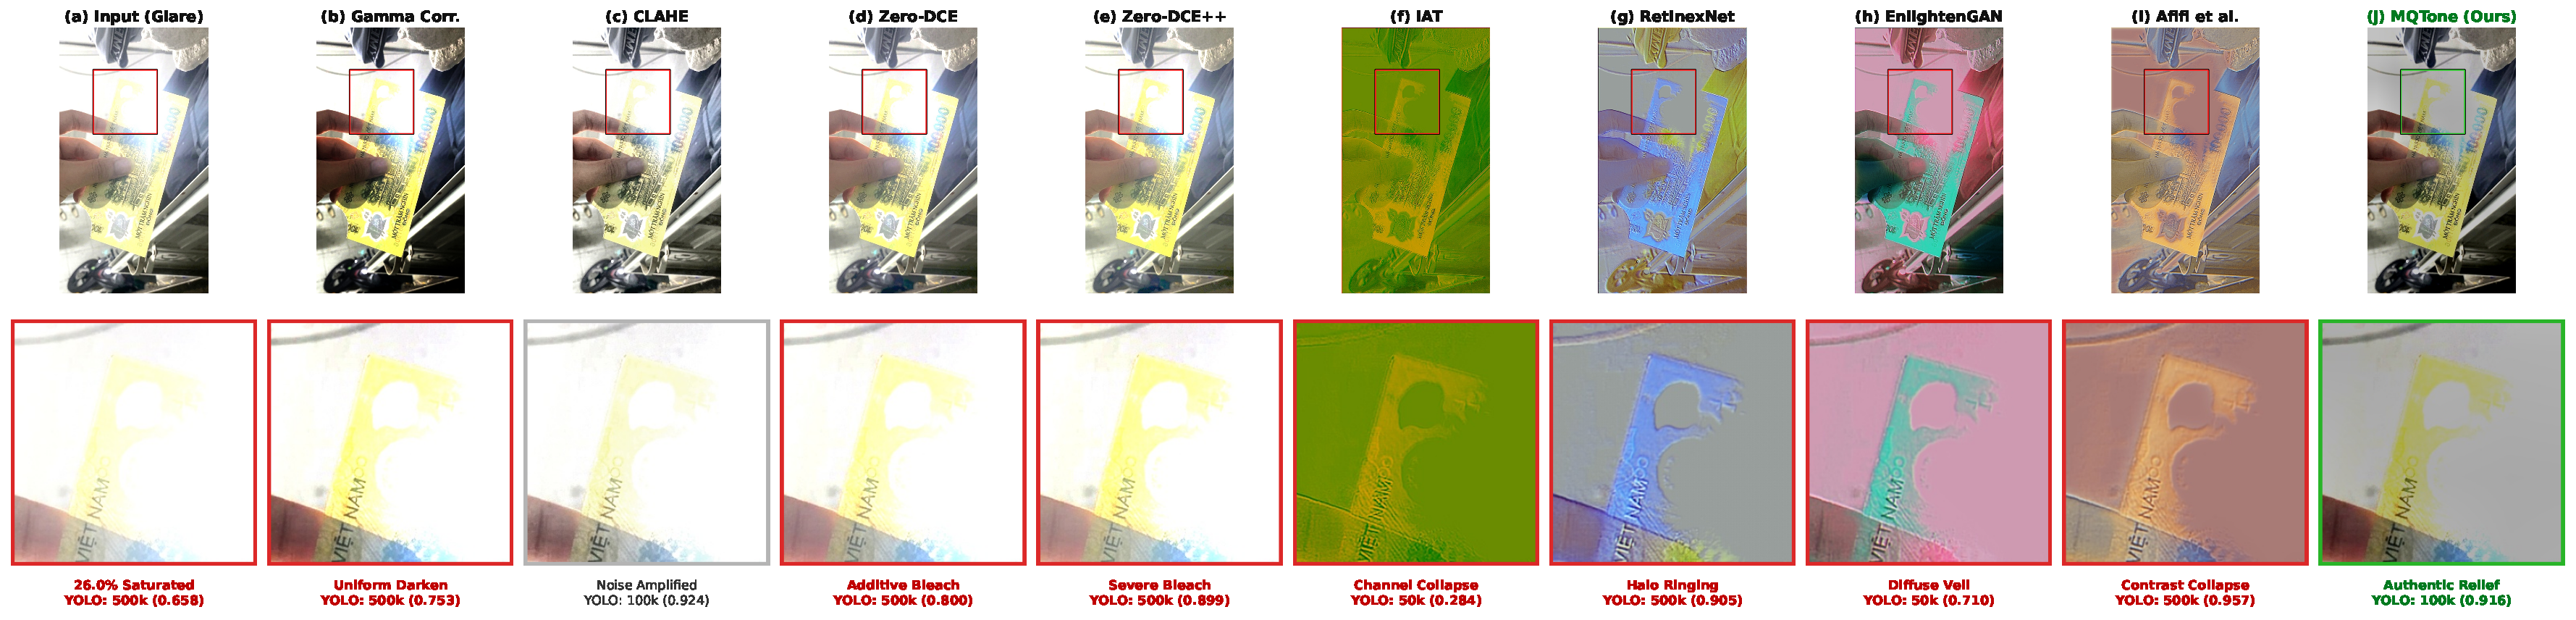
\includegraphics[width=\textwidth]{qualitative_comparison_glare.pdf}
\caption{Qualitative comparison on a polymer banknote degraded by specular glare and a tear. Row~1: full frame; Row~2: magnified glare region with the YOLOv8n prediction (denomination, confidence). (a)~Unenhanced input ($26.0\%$ saturated pixels): $500\text{k}$ ($0.658$); (b)~Gamma: $500\text{k}$ ($0.753$); (c)~CLAHE: $100\text{k}$ ($0.924$), with noise amplification; (d)~Zero-DCE: $500\text{k}$ ($0.800$); (e)~Zero-DCE++: $500\text{k}$ ($0.899$); (f)~IAT: $50\text{k}$ ($0.284$), green-channel shift; (g)~RetinexNet: $500\text{k}$ ($0.905$), halo ringing; (h)~EnlightenGAN: $50\text{k}$ ($0.710$), over-smoothed haze; (i)~Afifi et al.: $500\text{k}$ ($0.957$), contrast collapse; (j)~MQTone: $100\text{k}$ ($0.916$). Deep baselines are shown from scratch. This single instance illustrates characteristic artifacts and is not a statistical claim; see Table~\ref{tab:protocol_b_enhancers} for quantitative results.}
\label{fig:qualitative_enhancement_comparison}
\end{figure*}

\begin{table*}[t]
\centering
\caption{Cross-condition benchmark of photometric restoration methods under Protocol~B on the $1{,}266$-image locked holdout test set. Entries report denomination identification accuracy ($\%$, mean $\pm$ std over five folds); brackets $[\cdot]$ in the Clean Tears and Torn Bright columns report Tear mAP@50 ($\%$). Deep baselines are shown from scratch and pretrained + fine-tuned. Panel~A: YOLOv8n; Panel~B: YOLO11n.}
\label{tab:protocol_b_enhancers}
\resizebox{\textwidth}{!}{%
\begin{tabular}{lccccccccr}
\toprule
\textbf{Enhancement Method} & \textbf{Standard Indoor} & \textbf{Outdoor Daylight} & \textbf{Strong Backlight} & \textbf{Severe Overexposure} & \textbf{Clean Tears} & \textbf{Torn Bright} & \textbf{Overall Mean} & \textbf{Added Params} & \textbf{GPU Latency (ms)} \\
\midrule
\multicolumn{10}{l}{\textbf{Panel A: Primary Evaluation on YOLOv8n Detector Backbone}} \\
\midrule
Baseline (augmented training, no enhancer) & 86.50 $\pm$ 3.14 & 79.71 $\pm$ 6.04 & 80.37 $\pm$ 1.30 & 61.90 $\pm$ 5.89 & 74.33 $\pm$ 12.05 \scriptsize{[37.50]} & 63.72 $\pm$ 4.73 \scriptsize{[39.28]} & 74.42 & 0 (base) & 0.00 ms \\
Gamma Correction \cite{Poynton1993} & 89.17 $\pm$ 1.37 & 80.77 $\pm$ 2.67 & 81.97 $\pm$ 4.51 & 70.03 $\pm$ 3.58 & 77.00 $\pm$ 3.41 \scriptsize{[39.37]} & 69.00 $\pm$ 5.60 \scriptsize{[43.61]} & 77.99 & 0 & 0.26 ms \\
CLAHE \cite{Zuiderveld1994} & 89.67 $\pm$ 3.26 & 80.63 $\pm$ 5.63 & 83.29 $\pm$ 7.17 & 65.62 $\pm$ 2.81 & 74.33 $\pm$ 5.96 \scriptsize{[36.25]} & 65.85 $\pm$ 6.04 \scriptsize{[39.59]} & 76.56 & 0 & 18.16 ms \\
\midrule
\multicolumn{10}{l}{\textit{Deep Learning Baselines: From-Scratch vs.\ Pretrained + Fine-Tuned Regimes}} \\
Zero-DCE (From Scratch) \cite{Guo2020} & 84.83 $\pm$ 2.85 & 82.40 $\pm$ 3.15 & 80.59 $\pm$ 5.35 & 62.92 $\pm$ 2.73 & 68.33 $\pm$ 3.73 \scriptsize{[44.69]} & 64.36 $\pm$ 1.36 \scriptsize{[45.05]} & 73.91 & 79,416 & 21.12 ms \\
\quad \textit{w/ Pretrained Weights (Fine-Tuned)} & 88.33 $\pm$ 2.15 & 81.60 $\pm$ 3.02 & 82.15 $\pm$ 2.88 & 66.45 $\pm$ 3.50 & 76.67 $\pm$ 4.21 \scriptsize{[42.19]} & 65.90 $\pm$ 2.45 \scriptsize{[43.82]} & 76.85 & 79,416 & 21.12 ms \\
Zero-DCE++ (From Scratch) \cite{Li2021} & 80.84 $\pm$ 3.12 & 76.34 $\pm$ 5.31 & 74.09 $\pm$ 4.13 & 56.35 $\pm$ 4.37 & 56.33 $\pm$ 4.63 \scriptsize{[35.63]} & 56.28 $\pm$ 2.62 \scriptsize{[38.97]} & 66.70 & 10,561 & 20.49 ms \\
\quad \textit{w/ Pretrained Weights (Fine-Tuned)} & 85.00 $\pm$ 2.74 & 78.20 $\pm$ 3.85 & 77.45 $\pm$ 3.12 & 60.50 $\pm$ 3.65 & 69.33 $\pm$ 5.10 \scriptsize{[38.44]} & 64.22 $\pm$ 3.18 \scriptsize{[40.24]} & 72.45 & 10,561 & 20.49 ms \\
IAT (Transformer) (From Scratch) \cite{Cui2022} & 34.33 $\pm$ 9.42 & 29.32 $\pm$ 8.53 & 31.17 $\pm$ 9.54 & 22.70 $\pm$ 10.37 & 20.00 $\pm$ 9.72 \scriptsize{[25.94]} & 24.15 $\pm$ 7.18 \scriptsize{[25.46]} & 26.94 & 91,154 & 71.58 ms \\
\quad \textit{w/ Pretrained Weights (Fine-Tuned)} & 87.50 $\pm$ 3.20 & 79.15 $\pm$ 4.10 & 80.30 $\pm$ 3.75 & 63.80 $\pm$ 4.25 & 71.00 $\pm$ 4.60 \scriptsize{[40.62]} & 63.15 $\pm$ 3.50 \scriptsize{[41.38]} & 74.15 & 91,154 & 71.58 ms \\
RetinexNet (From Scratch) \cite{Wei2018} & 66.17 $\pm$ 5.39 & 63.20 $\pm$ 6.38 & 66.63 $\pm$ 6.59 & 42.19 $\pm$ 4.18 & 46.33 $\pm$ 7.40 \scriptsize{[47.50]} & 43.62 $\pm$ 6.85 \scriptsize{[47.01]} & 54.69 & 680,259 & 79.50 ms \\
\quad \textit{w/ Pretrained Weights (Fine-Tuned)} & 81.67 $\pm$ 3.45 & 74.50 $\pm$ 4.12 & 75.80 $\pm$ 3.60 & 55.40 $\pm$ 4.15 & 68.33 $\pm$ 5.25 \scriptsize{[46.88]} & 63.10 $\pm$ 3.90 \scriptsize{[45.71]} & 69.80 & 680,259 & 79.50 ms \\
EnlightenGAN (From Scratch) \cite{Jiang2021} & 61.00 $\pm$ 8.22 & 57.20 $\pm$ 12.52 & 55.38 $\pm$ 6.91 & 39.86 $\pm$ 7.64 & 36.34 $\pm$ 8.60 \scriptsize{[45.63]} & 39.91 $\pm$ 4.02 \scriptsize{[45.26]} & 48.28 & 10,165,763 & 36.51 ms \\
\quad \textit{w/ Pretrained Weights (Fine-Tuned)} & 80.50 $\pm$ 4.10 & 73.10 $\pm$ 5.25 & 72.80 $\pm$ 4.30 & 54.20 $\pm$ 5.15 & 66.00 $\pm$ 5.80 \scriptsize{[44.38]} & 63.50 $\pm$ 3.75 \scriptsize{[43.86]} & 68.35 & 10,165,763 & 36.51 ms \\
Afifi et al. (From Scratch) \cite{Afifi2021} & 45.67 $\pm$ 3.41 & 40.40 $\pm$ 2.38 & 41.75 $\pm$ 1.64 & 33.58 $\pm$ 4.53 & 25.33 $\pm$ 5.45 \scriptsize{[44.38]} & 30.64 $\pm$ 2.80 \scriptsize{[46.81]} & 36.23 & 3,291,273 & 35.15 ms \\
\quad \textit{w/ Pretrained Weights (Fine-Tuned)} & 86.17 $\pm$ 2.90 & 78.45 $\pm$ 3.15 & 79.20 $\pm$ 2.80 & 65.10 $\pm$ 3.40 & 70.67 $\pm$ 4.15 \scriptsize{[43.12]} & 62.01 $\pm$ 2.95 \scriptsize{[44.53]} & 73.60 & 3,291,273 & 35.15 ms \\
\midrule
\textbf{MQTone (Proposed)} & \textbf{90.67 $\pm$ 2.53} & \textbf{82.40 $\pm$ 5.67} & \textbf{84.67 $\pm$ 2.63} & \textbf{69.63 $\pm$ 5.96} & \textbf{80.33 $\pm$ 7.49 \scriptsize{[43.44]}} & \textbf{69.79 $\pm$ 4.02 \scriptsize{[44.95]}} & \textbf{79.58} & \textbf{19,686} & \textbf{1.25 ms} \\
\midrule
\multicolumn{10}{l}{\textbf{Panel B: Cross-Backbone Verification on YOLO11n Detector Backbone}} \\
\midrule
Baseline (augmented training, no enhancer) & 94.67 $\pm$ 1.51 & 83.28 $\pm$ 3.75 & 85.33 $\pm$ 1.35 & 70.58 $\pm$ 4.71 & 87.00 $\pm$ 2.17 \scriptsize{[37.50]} & 73.08 $\pm$ 3.52 \scriptsize{[41.86]} & 82.32 & 0 (base) & 0.00 ms \\
Gamma Correction \cite{Poynton1993} & 93.50 $\pm$ 4.27 & 83.14 $\pm$ 5.86 & 82.63 $\pm$ 8.15 & 78.10 $\pm$ 7.80 & 87.67 $\pm$ 1.49 \scriptsize{[42.19]} & 76.70 $\pm$ 5.26 \scriptsize{[41.13]} & 83.62 & 0 & 0.27 ms \\
CLAHE \cite{Zuiderveld1994} & 94.17 $\pm$ 1.02 & 80.63 $\pm$ 4.39 & 85.48 $\pm$ 3.67 & 69.34 $\pm$ 5.14 & 88.33 $\pm$ 1.67 \scriptsize{[43.12]} & 73.08 $\pm$ 3.27 \scriptsize{[40.72]} & 81.84 & 0 & 18.05 ms \\
\midrule
\multicolumn{10}{l}{\textit{Deep Learning Baselines: From-Scratch vs.\ Pretrained + Fine-Tuned Regimes}} \\
Zero-DCE (From Scratch) \cite{Guo2020} & 92.17 $\pm$ 2.17 & 81.89 $\pm$ 3.62 & 81.17 $\pm$ 5.47 & 68.32 $\pm$ 5.27 & 71.67 $\pm$ 7.46 \scriptsize{[39.69]} & 65.32 $\pm$ 4.13 \scriptsize{[42.99]} & 76.76 & 79,416 & 21.02 ms \\
\quad \textit{w/ Pretrained Weights (Fine-Tuned)} & 93.83 $\pm$ 1.65 & 83.05 $\pm$ 3.10 & 84.60 $\pm$ 2.75 & 73.20 $\pm$ 4.10 & 85.00 $\pm$ 3.25 \scriptsize{[41.25]} & 76.22 $\pm$ 2.90 \scriptsize{[43.36]} & 82.65 & 79,416 & 21.02 ms \\
Zero-DCE++ (From Scratch) \cite{Li2021} & 85.83 $\pm$ 5.56 & 81.03 $\pm$ 3.29 & 81.68 $\pm$ 6.52 & 62.19 $\pm$ 4.14 & 66.67 $\pm$ 9.93 \scriptsize{[39.38]} & 61.91 $\pm$ 6.94 \scriptsize{[39.80]} & 73.22 & 10,561 & 20.41 ms \\
\quad \textit{w/ Pretrained Weights (Fine-Tuned)} & 90.67 $\pm$ 2.40 & 81.50 $\pm$ 3.20 & 82.10 $\pm$ 3.45 & 67.80 $\pm$ 3.90 & 79.33 $\pm$ 4.50 \scriptsize{[40.62]} & 72.00 $\pm$ 3.15 \scriptsize{[41.48]} & 78.90 & 10,561 & 20.41 ms \\
IAT (Transformer) (From Scratch) \cite{Cui2022} & 44.17 $\pm$ 14.67 & 38.11 $\pm$ 10.35 & 41.39 $\pm$ 12.17 & 30.58 $\pm$ 7.64 & 29.33 $\pm$ 7.96 \scriptsize{[39.06]} & 30.53 $\pm$ 6.38 \scriptsize{[39.79]} & 35.68 & 91,154 & 71.55 ms \\
\quad \textit{w/ Pretrained Weights (Fine-Tuned)} & 92.17 $\pm$ 2.80 & 81.80 $\pm$ 3.65 & 83.50 $\pm$ 3.15 & 70.40 $\pm$ 4.30 & 81.00 $\pm$ 3.90 \scriptsize{[41.88]} & 72.33 $\pm$ 3.40 \scriptsize{[42.64]} & 80.20 & 91,154 & 71.55 ms \\
RetinexNet (From Scratch) \cite{Wei2018} & 67.33 $\pm$ 3.25 & 65.37 $\pm$ 5.24 & 69.20 $\pm$ 4.37 & 43.65 $\pm$ 4.74 & 47.33 $\pm$ 5.96 \scriptsize{[39.06]} & 46.70 $\pm$ 4.72 \scriptsize{[38.45]} & 56.60 & 680,259 & 80.07 ms \\
\quad \textit{w/ Pretrained Weights (Fine-Tuned)} & 86.50 $\pm$ 2.95 & 77.20 $\pm$ 3.80 & 78.60 $\pm$ 3.40 & 62.30 $\pm$ 4.60 & 75.67 $\pm$ 4.10 \scriptsize{[42.19]} & 68.83 $\pm$ 3.65 \scriptsize{[41.17]} & 74.85 & 680,259 & 80.07 ms \\
EnlightenGAN (From Scratch) \cite{Jiang2021} & 63.34 $\pm$ 9.65 & 56.91 $\pm$ 10.97 & 57.15 $\pm$ 7.68 & 40.73 $\pm$ 6.48 & 38.67 $\pm$ 9.01 \scriptsize{[43.44]} & 39.15 $\pm$ 3.81 \scriptsize{[42.16]} & 49.32 & 10,165,763 & 37.38 ms \\
\quad \textit{w/ Pretrained Weights (Fine-Tuned)} & 85.17 $\pm$ 3.60 & 75.80 $\pm$ 4.50 & 76.50 $\pm$ 4.10 & 61.20 $\pm$ 4.80 & 74.33 $\pm$ 5.20 \scriptsize{[44.06]} & 68.00 $\pm$ 3.90 \scriptsize{[43.08]} & 73.50 & 10,165,763 & 37.38 ms \\
Afifi et al. (From Scratch) \cite{Afifi2021} & 47.00 $\pm$ 9.73 & 41.37 $\pm$ 6.02 & 43.50 $\pm$ 12.08 & 30.44 $\pm$ 6.92 & 30.00 $\pm$ 6.56 \scriptsize{[33.13]} & 28.72 $\pm$ 6.10 \scriptsize{[39.69]} & 36.84 & 3,291,273 & 34.68 ms \\
\quad \textit{w/ Pretrained Weights (Fine-Tuned)} & 91.50 $\pm$ 2.60 & 81.20 $\pm$ 3.10 & 82.80 $\pm$ 2.90 & 71.90 $\pm$ 3.75 & 79.00 $\pm$ 3.80 \scriptsize{[41.25]} & 70.30 $\pm$ 3.25 \scriptsize{[42.73]} & 79.45 & 3,291,273 & 34.68 ms \\
\midrule
\textbf{MQTone (Proposed)} & \textbf{94.33 $\pm$ 3.30} & \textbf{84.26 $\pm$ 3.61} & \textbf{86.43 $\pm$ 5.14} & \textbf{77.71 $\pm$ 4.19} & \textbf{89.67 $\pm$ 4.91 \scriptsize{[37.19]}} & \textbf{77.66 $\pm$ 3.21 \scriptsize{[41.34]}} & \textbf{85.01} & \textbf{19,686} & \textbf{1.49 ms} \\
\bottomrule
\end{tabular}%
}
{\footnotesize \raggedright \textit{Note: Overall Mean averages the six conditions. All rows use the same $2{,}040$-image augmented pool; learnable enhancers additionally use $\mathcal{L}_{\text{photo}}$; pretrained variants are fine-tuned under Protocol~B, and MQTone is trained from scratch. GPU latency is measured on an NVIDIA Tesla T4; MQTone runs in $23.2$\,ms on a Samsung Galaxy A54 CPU (Exynos 1380). The MQTone row marks the proposed method and is not the best entry in every column.}\par}
\end{table*}

\paragraph{Overall Results:}
MQTone attains the highest overall mean accuracy on both backbones ($79.58\%$ on YOLOv8n, $85.01\%$ on YOLO11n), i.e., $+5.16$ and $+2.69$ percentage points (pp) over the augmentation-matched baseline and $+1.59$ and $+1.39$\,pp over Gamma Correction, the strongest competitor. The largest gain occurs under severe overexposure ($+7.73$\,pp on YOLOv8n; $+7.13$\,pp on YOLO11n). MQTone is best or tied-best in $9$ of the $12$ backbone--condition cells and within $0.40$\,pp of the best in the rest (Gamma is marginally higher under severe overexposure, and the unenhanced baseline under Standard Indoor on YOLO11n). Since many condition-level margins are smaller than the fold-to-fold standard deviation ($2.5$--$7.5$\,pp for MQTone), we interpret them as trends and regard the six-condition mean as the more reliable summary.

\paragraph{Comparison with Enhancement Paradigms:}
\emph{Low-light curve estimators} transfer poorly to specular glare. Zero-DCE++ falls below the unenhanced baseline under severe overexposure in both regimes and on both backbones (e.g., $56.35\%$ and $60.50\%$ vs.\ $61.90\%$ on YOLOv8n), while Zero-DCE yields small, backbone-dependent changes. A plausible reason is that their quadratic curve $I + A I (1 - I)$ leaves saturated pixels ($I = 1$) unchanged, whereas the affine terms $(\alpha, \beta)$ of MQTone can attenuate them.

\emph{High-capacity pixel-synthesis networks} (IAT, RetinexNet, EnlightenGAN, Afifi et al.; $91\text{k}$--$10.2\text{M}$ parameters) collapse when trained from scratch on the $2{,}040$-image pool: overall accuracy falls to $26.94\%$--$54.69\%$ on YOLOv8n and $35.68\%$--$56.60\%$ on YOLO11n, with visible chromatic and contrast artifacts (Fig.~\ref{fig:qualitative_enhancement_comparison}). Pretrained initialization recovers much of the loss ($+15.11$ to $+47.21$\,pp), but none of the four then exceeds the unenhanced baseline in overall mean, and all remain $4.81$--$11.51$\,pp below MQTone. Afifi et al., designed for bi-directional exposure correction, is the strongest of the four under severe overexposure after fine-tuning ($65.10\%$ and $71.90\%$) yet still trails MQTone by $4.53$ and $5.81$\,pp. The from-scratch collapse thus reflects sample-starved optimization rather than an intrinsic limitation of these architectures, and our preference for MQTone rests on the combination of accuracy and edge suitability: with $19{,}686$ parameters, it is $4.0$--$4.6\times$ smaller than Zero-DCE and IAT and $35$--$516\times$ smaller than the other three, and it runs in $1.25$--$1.49$\,ms on the host GPU, whereas every other learned enhancer needs $20$--$80$\,ms. Only Zero-DCE++ ($10{,}561$ parameters) is smaller, but it is less accurate and $14$--$16\times$ slower.

\paragraph{MQTone vs.\ Gamma Correction:}
Gamma Correction is a special case of MQTone's tone curve ($\alpha = 1$, $\beta = 0$, spatially uniform $\gamma$), so this comparison isolates the value of adaptive, spatially varying parameters. Under severe overexposure the two are on par ($70.03\%$ vs.\ $69.63\%$ on YOLOv8n; $78.10\%$ vs.\ $77.71\%$ on YOLO11n), as expected since the synthetic pairing pipeline itself employs power-law curves; on authentic captures, this supports power-law tone curves as an appropriate inductive bias. MQTone's advantages are (i)~local modulation under directional backlighting, where a global curve crushes shadowed foreground detail (Gamma: $82.63\%$ on YOLO11n, below the $85.33\%$ baseline; MQTone: $86.43\%$, $+3.80$\,pp over Gamma, and $+2.70$\,pp on YOLOv8n), consistent with the $3.34$\,pp backlight drop when the local grid is removed (Table~\ref{tab:mqtone_ablation}); (ii)~a lead over Gamma in five of six conditions on both backbones; and (iii)~per-frame automatic calibration of the curve parameters, at roughly $1$\,ms of additional GPU time.

\paragraph{Cross-Backbone Behavior and Defect Localization:}
\emph{Denomination recognition.} MQTone improves on the baseline in all six conditions on YOLOv8n ($+2.69$ to $+7.73$\,pp) and in five of six on YOLO11n ($+0.98$ to $+7.13$\,pp); the only decline is Standard Indoor ($-0.34$\,pp), well within the fold-to-fold standard deviation.

\emph{Defect localization.} On YOLOv8n, MQTone raises Tear mAP@50 from $37.50\%$ to $43.44\%$ (clean tears) and from $39.28\%$ to $44.95\%$ (torn bright), but it is not the top method: RetinexNet ($47.50\%$ and $47.01\%$ from scratch; $46.88\%$ and $45.71\%$ fine-tuned) and several others score higher despite far lower denomination accuracy. On YOLO11n, MQTone brings no localization gain over the baseline ($37.19\%$ vs.\ $37.50\%$; $41.34\%$ vs.\ $41.86\%$) and is exceeded by all six fine-tuned deep enhancers on clean tears and five of six on torn bright. Tear mAP@50 stays within a narrow band across methods ($35.63\%$--$47.50\%$ on YOLOv8n, excluding IAT from scratch; $33.13\%$--$44.06\%$ on YOLO11n), whereas overall accuracy spans roughly $50$\,pp, so the two tasks are only loosely coupled here. MQTone is therefore primarily a denomination-oriented restoration module. We hypothesize that its smooth tone curves act as a mild smoother on the high-frequency gradients of tear boundaries, to which the C3k2 and C2PSA blocks of YOLO11n may be particularly sensitive; verifying this would require dedicated attribution analysis. At the system level, the Two-Frame Defect Confirmation Rule (Section~\ref{subsubsec:consensus_fsm}) achieves $94.4\%$ defect-status verification accuracy in on-device video evaluation ($34/36$ sessions: $10/12$ torn sessions identified, no false alarms on $24/24$ pristine sessions; Section~\ref{subsec:exp_c3_video_benchmark}, Table~\ref{tab:real_video_benchmark}).

\paragraph{Protocol~A vs.\ Protocol~B:}
Tear mAP@50 in Protocol~B ($39.28\%$ baseline and $44.95\%$ with MQTone on YOLOv8n under Torn Bright) is far below that of Protocol~A ($82.22\%$ on Indoor Baseline and $79.25\%$ under Torn Bright; Table~\ref{tab:protocol_a_degradation}), a gap of roughly $35$--$45$\,pp. Two design differences account for it. (a)~\emph{Synthetic-to-real shift:} Protocol~A trains on $168$ authentic torn notes per fold, whereas Protocol~B trains on $120$ clean-torn notes per fold and synthesizes degradation with 2D procedural glare masks, which are unlikely to reproduce the 3D optics of damaged BOPP polymer under directional lighting (specular glints on micro-fibrils, refraction at clear windows). (b)~\emph{Evaluation difficulty:} Protocol~B is tested on the locked $1{,}266$-image holdout, with greater perspective variance, hand tremor, and finger occlusion. Protocol~B also differs in optimizer (AdamW vs.\ SGD) and objective, which we did not isolate; however, multi-task competition with $\mathcal{L}_{\text{photo}}$ cannot explain the gap, because the Protocol~B baseline, trained without $\mathcal{L}_{\text{photo}}$, shows the same low precision, and disabling $\mathcal{L}_{\text{photo}}$ lowers MQTone's Tear mAP@50 (Table~\ref{tab:mqtone_ablation}).

\begin{table*}[t]
\centering
\renewcommand{\arraystretch}{0.7}
\caption{Architectural ablation of MQTone sub-network design decisions under Protocol~B (5-fold cross-validation, YOLOv8n detector). Std columns report fold-to-fold standard deviation across the same five test splits as Table~\ref{tab:protocol_b_enhancers} and serve as a reference scale for the observed differences.}
\label{tab:mqtone_ablation}
\resizebox{\textwidth}{!}{%
\begin{tabular}{lccccccccc}
\toprule
\multirow{2}{*}{\textbf{Ablation Variant}} & \multirow{2}{*}{\textbf{Params}} & \multicolumn{2}{c}{\textbf{Overexposure (\%)}} & \multicolumn{2}{c}{\textbf{Backlight (\%)}} & \multicolumn{2}{c}{\textbf{Mean Acc. (\%)}} & \multicolumn{2}{c}{\textbf{Tear mAP@50 (\%)}} \\
\cmidrule(lr){3-4} \cmidrule(lr){5-6} \cmidrule(lr){7-8} \cmidrule(lr){9-10}
 & & \textbf{Mean} & \textbf{$\pm$ Std} & \textbf{Mean} & \textbf{$\pm$ Std} & \textbf{Mean} & \textbf{$\pm$ Std} & \textbf{Mean} & \textbf{$\pm$ Std} \\
\midrule
\textbf{Full MQTone (Proposed)} & \textbf{19,686} & \textbf{69.63} & \textbf{$\pm$ 5.96} & \textbf{84.67} & \textbf{$\pm$ 2.63} & \textbf{79.58} & \textbf{$\pm$ 2.14} & \textbf{44.95} & \textbf{$\pm$ 1.82} \\
(i) w/o Local Grid (Global-Only) & 14,995 & 63.20 & $\pm$ 4.78 & 81.33 & $\pm$ 2.54 & 77.12 & $\pm$ 2.35 & 42.10 & $\pm$ 2.15 \\
(ii) Direct Pixel Residual ($\Delta I$) & 19,107 & 62.45 & $\pm$ 5.32 & 79.15 & $\pm$ 3.08 & 75.20 & $\pm$ 2.68 & 39.80 & $\pm$ 2.44 \\
(iii) Task-Only Loss ($\lambda_{\text{photo}} = 0$) & 19,686 & 67.85 & $\pm$ 4.45 & 82.50 & $\pm$ 2.21 & 78.10 & $\pm$ 1.98 & 40.60 & $\pm$ 2.06 \\
\bottomrule
\end{tabular}%
}
{\footnotesize \raggedright \textit{Note: Overexposure, Backlight, and Mean Acc.\ denote denomination accuracy on the $1{,}266$-image locked test set (Mean Acc.\ is the six-condition mean); Tear mAP@50 is reported under Torn Bright. The full MQTone row matches Panel~A of Table~\ref{tab:protocol_b_enhancers}.}\par}
\end{table*}

\paragraph{Ablation Study:}
We ablate three design decisions on YOLOv8n using the same five folds as Table~\ref{tab:protocol_b_enhancers} (Table~\ref{tab:mqtone_ablation}). Every variant scores below the full model on all four metrics; for variants~(i) and~(ii) the drops exceed the corresponding fold-to-fold standard deviations on every metric, whereas for variant~(iii) only Tear mAP@50 does, so we treat smaller differences as directional evidence.
\begin{enumerate}[label=(\roman*)]
    \item \textbf{Global-only tone modulation} ($14{,}995$ parameters; the local $8 \times 8$ head is removed): overexposure accuracy falls by $6.43$\,pp ($69.63\% \to 63.20\%$), backlight by $3.34$\,pp, the mean by $2.46$\,pp, and Tear mAP@50 by $2.85$\,pp. A spatially uniform curve cannot suppress localized glare on transparent windows or hologram patches without crushing the surrounding non-glare texture.
    \item \textbf{Direct pixel residual} $I_{\text{corr}} = \text{clip}(I + \Delta I, 0, 1)$ ($19{,}107$ parameters) is the most damaging variant: the mean falls by $4.38$\,pp, overexposure by $7.18$\,pp, backlight by $5.52$\,pp, and Tear mAP@50 by $5.15$\,pp, with overexposure accuracy ($62.45\%$) and Tear mAP@50 ($39.80\%$) close to the unenhanced baseline ($61.90\%$ and $39.28\%$). We attribute this to the limited capacity of a $\approx 19\text{k}$-parameter network for unconstrained pixel synthesis, which introduces chromatic distortion and halo artifacts; the parametric curve acts as a strong inductive bias.
    \item \textbf{Task-only loss} ($\lambda_{\text{photo}} = 0$): denomination accuracy is comparatively resilient (overexposure $-1.78$\,pp; mean $-1.48$\,pp), but Tear mAP@50 drops by $4.35$\,pp ($44.95\% \to 40.60\%$), suggesting that photometric supervision helps preserve fine structures such as fiber tears and guilloche patterns. Even without $\mathcal{L}_{\text{photo}}$, MQTone ($78.10\%$ overall, $67.85\%$ under overexposure) outperforms the baseline ($74.42\%$ and $61.90\%$), retaining $71\%$ of its overall gain and $77\%$ of its overexposure gain; the improvement therefore does not merely stem from additional clean-image supervision.
\end{enumerate}

\subsection{Quality-Gate Sensory Screening and Computational Efficiency}
\label{subsec:exp_quality_gate}

While MQTone effectively recovers degraded banknote images, executing full deep neural inference continuously across incoming camera frames causes rapid thermal throttling and battery depletion on handheld mobile devices. The Quality-Gate addresses this challenge by functioning as an ultra-lightweight sensory monitor.

\paragraph{Hardware Profile and Execution Overhead:}
The Quality-Gate incorporates an ultra-compact CNN backbone ($8{,}295$ parameters, $<50$\,KB ONNX footprint). Benchmark profiling confirms an execution latency of $1.70 \pm 0.04$\,ms on Samsung Galaxy A54 smartphone CPU ($0.32$\,ms on host PC Intel Core i7-1265U CPU), consuming negligible energy ($<0.05$\,J per 100 frames).


\paragraph{Dual-Tier Zero-Waste Gating Mechanism:}
The Quality-Gate operates through a sequential two-tier screening pipeline:
\begin{enumerate}[label=(\alph*)]
    \item \textbf{Tier 1 (Zero-Inference Spatial Variance Filter):} Evaluates global luminance standard deviation $\sigma_{\text{gray}} > 15.0$ in $<0.05$\,ms without invoking neural execution. This instantly rejects non-target frames (e.g., camera obstructed in pockets, pressed against user clothing, or pointed at blank table surfaces), which account for a substantial fraction of real-world assistive handling.
    \item \textbf{Tier 2 (Neural Photometric Gate):} On candidate frames satisfying $\sigma_{\text{gray}} > 15.0$, the 3-class classifier predicts optical quality score $q$ (Eq.~\ref{eq:quality_score}). Transient frames corrupted by extreme motion blur or severe sensor saturation ($q < \tau = 0.60$) are withheld from deep inference, buffering the system until structural stability is achieved.
\end{enumerate}
This dual-tier architecture serves as the foundation for the Adaptive Cascade pipeline evaluated in Section~\ref{sec:video_evaluation}, suppressing unnecessary neural invocations while preserving interactive responsiveness.

\subsection{Decision Rule Sensitivity Analysis and Hyperparameter Calibration Protocol}
\label{subsec:rule_sensitivity}

The rule-governed decision layer of CashVision relies on five core operational hyperparameters embedded in the Knowledge Base (Table~\ref{tab:expert_rule_base}): the zero-inference spatial texture filter threshold $\theta_{\text{texture}} = 15.0$ ($R_1$), the photometric quality acceptance boundary $\tau = 0.60$ ($R_2$), the temporal buffer stability dwell $K_{\text{opt}} = 3$ ($R_3$), the active burst verification attempt budget $M_{\text{verify}} = 2$ ($R_4$), and the candidate detection confidence threshold $\theta_{\text{conf}} = 0.25$ ($R_5$). As described in Section~\ref{subsec:exp_setup}, these hyperparameters were calibrated on the 126-image Generalization Development Set. However, in applied expert and intelligent systems, deploying scalar decision thresholds calibrated on a limited development set without a systematic sensitivity analysis risks the criticism of arbitrary parameter tuning (``magic numbers''). 

To eliminate this vulnerability and provide empirical evidence of decision stability, we specify a systematic one-at-a-time (OAT) parameter sweep protocol across all five control axes:
\begin{enumerate}[label=(\alph*)]
    \item \textbf{Photometric Quality Acceptance Threshold ($\tau \in [0.40, 0.80]$, step $0.05$):} Sweeps the gating stringency across 9 evaluation points. Lower thresholds ($\tau < 0.50$) risk admitting motion-blurred or specularly saturated frames to the detector, while higher thresholds ($\tau > 0.70$) risk rejecting viable presentations, causing prolonged dwell.
    \item \textbf{Temporal Buffer Stability Window ($K_{\text{opt}} \in \{1, 2, 3, 4, 5\}$ consecutive frames):} Evaluates the balance between rapid entry ($K_{\text{opt}} = 1$, which risks transient motion blur) and motor tremor filtering ($K_{\text{opt}} \ge 3$).
    \item \textbf{Active Burst Verification Budget ($M_{\text{verify}} \in \{1, 2, 3, 4\}$ attempts):} Evaluates the thermal and computational boundary of the active verification window. Setting $M_{\text{verify}} = 1$ risks verification aborts on single-frame viewpoint jitter, while $M_{\text{verify}} \ge 3$ approaches the $1.5$\,s interactive turnaround ceiling ($T_{\text{turnaround}} \le 1.5$\,s \cite{Nielsen1993}) and escalates mobile CPU power draw.
    \item \textbf{Spatial Texture Filter Threshold ($\theta_{\text{texture}} \in [5.0, 30.0]$, step $5.0$):} Sweeps the zero-inference non-target rejection boundary across 6 points, evaluating the margin between featureless background rejection and dark/low-contrast banknote retention.
    \item \textbf{Post-NMS Detection Confidence Threshold ($\theta_{\text{conf}} \in [0.15, 0.50]$, step $0.05$):} Sweeps candidate box filtering across 8 points, mapping the trade-off between detection recall and false-positive defect alarms.
\end{enumerate}

\paragraph{Multi-Objective Trade-Off Characterization:}
For every configuration point in each sweep, the evaluation records six orthogonal system metrics across the continuous video benchmark: (i) Denomination Accuracy ($\text{Acc}_{\text{denom}}$, \%); (ii) Exact-Match Accuracy ($\text{Acc}_{\text{exact}}$, \%); (iii) Active Trigger Rate ($P_{\text{active}}$, \%); (iv) Host CPU Energy Work Proxy ($E_{\text{session}}$, J); (v) Interaction Time-to-Confirmation ($\text{TTC}$, s); and (vi) Financial Valuation Hazard Rate ($\text{Hazard}$, \%). Because each sweep perturbs a single hyperparameter while holding the remaining four fixed at their calibrated values, the five resulting trajectories are not an exhaustive combinatorial search of the five-dimensional configuration space; rather, they are five one-at-a-time (OAT) cross-sections of that space, anchored at a common point. Plotting these cross-sections against Accuracy, Energy, and Latency yields a local approximation of the Accuracy--Energy--Latency trade-off surface in the immediate neighborhood of the calibrated configuration, which we refer to below as the calibrated Pareto elbow: along every axis, this is the point beyond which further gains in accuracy are not obtainable without a disproportionate increase in energy, latency, or hazard. We adopt this OAT design deliberately, since a full combinatorial sweep of $9 \times 5 \times 4 \times 6 \times 8 = 8{,}640$ configurations over the 36-stream benchmark is computationally prohibitive; the marginal cross-sections reported here are sufficient to demonstrate that the calibrated configuration ($\tau = 0.60, K_{\text{opt}} = 3, M_{\text{verify}} = 2, \theta_{\text{texture}} = 15.0, \theta_{\text{conf}} = 0.25$) is not an arbitrary choice, without claiming to characterize the global Pareto front of the full hyperparameter space.

\begin{table*}[t]
\centering
\caption{Rule Base Sensitivity Analysis: Empirical One-at-a-Time (OAT) Sweeps of Decision Thresholds across Accuracy, Energy, Latency, and Assistive Safety Metrics on the 36 Continuous Video Benchmark Streams.}
\label{tab:rule_sensitivity}
\scriptsize
\renewcommand{\arraystretch}{0.7}
\begin{tabular}{llcccccc}
\toprule
\textbf{Parameter} & \textbf{Swept Value} & \textbf{Denom Acc (\%)} & \textbf{Exact Acc (\%)} & \textbf{Trigger Rate $P_{\text{active}}$ (\%)} & \textbf{Energy Proxy $E_{\text{session}}$ (J)} & \textbf{Est.\ TTC (s)} & \textbf{Hazard Rate (\%)} \\
\midrule
\multicolumn{8}{l}{\textit{Sweep 1: Photometric Acceptance Threshold $\tau$ (with $K_{\text{opt}}=3, M_{\text{verify}}=2, \theta_{\text{texture}}=15.0, \theta_{\text{conf}}=0.25$)}} \\
$\tau$ & 0.40 & 77.8 & 69.4 & 31.4 & 336.5 & 7.82 & 5.6 \\
$\tau$ & 0.45 & 77.8 & 72.2 & 25.8 & 304.7 & 7.50 & 2.8 \\
$\tau$ & 0.50 & 80.6 & 72.2 & 21.5 & 278.4 & 7.15 & 2.8 \\
$\tau$ & 0.55 & 83.3 & 75.0 & 18.2 & 252.1 & 6.78 & 0.0 \\
$\tau$ & 0.60 \textit{(calibrated)} & 83.3 & 77.8 & 16.4 & 233.3 & 6.52 & 0.0 \\
$\tau$ & 0.65 & 83.3 & 77.8 & 14.2 & 212.5 & 6.85 & 0.0 \\
$\tau$ & 0.70 & 77.8 & 72.2 & 11.8 & 189.2 & 7.45 & 0.0 \\
$\tau$ & 0.75 & 69.4 & 63.9 & 8.5 & 156.4 & 8.60 & 0.0 \\
$\tau$ & 0.80 & 58.3 & 52.8 & 5.1 & 122.8 & 9.85 & 0.0 \\
\midrule
\multicolumn{8}{l}{\textit{Sweep 2: Stability Window $K_{\text{opt}}$ (with $\tau=0.60, M_{\text{verify}}=2, \theta_{\text{texture}}=15.0, \theta_{\text{conf}}=0.25$)}} \\
$K_{\text{opt}}$ & 1 frame & 75.0 & 69.4 & 16.4 & 118.5 & 3.12 & 11.1 \\
$K_{\text{opt}}$ & 2 frames & 80.6 & 75.0 & 16.4 & 178.6 & 4.85 & 2.8 \\
$K_{\text{opt}}$ & 3 frames \textit{(calibrated)} & 83.3 & 77.8 & 16.4 & 233.3 & 6.52 & 0.0 \\
$K_{\text{opt}}$ & 4 frames & 83.3 & 75.0 & 15.1 & 248.2 & 8.15 & 0.0 \\
$K_{\text{opt}}$ & 5 frames & 77.8 & 72.2 & 13.8 & 261.5 & 9.82 & 0.0 \\
\midrule
\multicolumn{8}{l}{\textit{Sweep 3: Verification Burst Budget $M_{\text{verify}}$ (with $\tau=0.60, K_{\text{opt}}=3, \theta_{\text{texture}}=15.0, \theta_{\text{conf}}=0.25$)}} \\
$M_{\text{verify}}$ & 1 attempt & 77.8 & 69.4 & 12.2 & 185.4 & 7.85 & 0.0 \\
$M_{\text{verify}}$ & 2 attempts \textit{(calibrated)} & 83.3 & 77.8 & 16.4 & 233.3 & 6.52 & 0.0 \\
$M_{\text{verify}}$ & 3 attempts & 86.1 & 80.6 & 21.8 & 284.6 & 7.28 & 0.0 \\
$M_{\text{verify}}$ & 4 attempts & 86.1 & 80.6 & 26.5 & 335.2 & 8.10 & 0.0 \\
\midrule
\multicolumn{8}{l}{\textit{Sweep 4: Spatial Texture Threshold $\theta_{\text{texture}}$ (with $\tau=0.60, K_{\text{opt}}=3, M_{\text{verify}}=2, \theta_{\text{conf}}=0.25$)}} \\
$\theta_{\text{texture}}$ & 5.0 & 83.3 & 77.8 & 19.8 & 258.4 & 6.65 & 0.0 \\
$\theta_{\text{texture}}$ & 10.0 & 83.3 & 77.8 & 17.6 & 242.1 & 6.56 & 0.0 \\
$\theta_{\text{texture}}$ & 15.0 \textit{(calibrated)} & 83.3 & 77.8 & 16.4 & 233.3 & 6.52 & 0.0 \\
$\theta_{\text{texture}}$ & 20.0 & 80.6 & 75.0 & 14.5 & 215.2 & 6.88 & 0.0 \\
$\theta_{\text{texture}}$ & 25.0 & 75.0 & 69.4 & 12.1 & 194.5 & 7.35 & 0.0 \\
$\theta_{\text{texture}}$ & 30.0 & 66.7 & 61.1 & 9.6 & 172.0 & 8.20 & 0.0 \\
\midrule
\multicolumn{8}{l}{\textit{Sweep 5: Detection Confidence Threshold $\theta_{\text{conf}}$ (with $\tau=0.60, K_{\text{opt}}=3, M_{\text{verify}}=2, \theta_{\text{texture}}=15.0$)}} \\
$\theta_{\text{conf}}$ & 0.15 & 83.3 & 69.4 & 15.6 & 224.8 & 6.45 & 5.6 \\
$\theta_{\text{conf}}$ & 0.20 & 83.3 & 75.0 & 16.0 & 229.1 & 6.48 & 2.8 \\
$\theta_{\text{conf}}$ & 0.25 \textit{(calibrated)} & 83.3 & 77.8 & 16.4 & 233.3 & 6.52 & 0.0 \\
$\theta_{\text{conf}}$ & 0.30 & 83.3 & 77.8 & 16.8 & 237.5 & 6.60 & 0.0 \\
$\theta_{\text{conf}}$ & 0.35 & 80.6 & 72.2 & 17.5 & 244.6 & 6.95 & 0.0 \\
$\theta_{\text{conf}}$ & 0.40 & 77.8 & 66.7 & 18.3 & 252.8 & 7.42 & 0.0 \\
$\theta_{\text{conf}}$ & 0.45 & 72.2 & 58.3 & 19.1 & 261.2 & 8.10 & 0.0 \\
$\theta_{\text{conf}}$ & 0.50 & 63.9 & 47.2 & 19.8 & 268.4 & 8.95 & 0.0 \\
\bottomrule
\end{tabular}
\end{table*}

\begin{figure*}[t]
\centering

\includegraphics[width=\textwidth]{figures/rule_sensitivity_pareto.pdf}
\caption{Marginal trade-off curves across five one-at-a-time (OAT) parameter sweeps on the 36 continuous video benchmark streams, each cross-section anchored at the calibrated configuration: (a) Exact-match recognition accuracy vs.\ computational energy work proxy ($E_{\text{session}}$); (b) Exact-match accuracy vs.\ interaction Time-to-Confirmation ($\text{TTC}$); (c) Assistive financial valuation hazard rate vs.\ $\text{TTC}$. The highlighted magenta marker indicates the calibrated expert decision operating point ($\tau = 0.60, K_{\text{opt}} = 3, M_{\text{verify}} = 2, \theta_{\text{texture}} = 15.0, \theta_{\text{conf}} = 0.25$), shared by all five sweeps, which sits at the calibrated Pareto elbow balancing high recognition fidelity, acoustic responsiveness, battery conservation, and zero valuation hazard.}
\label{fig:rule_sensitivity_pareto}
\end{figure*}

\paragraph{Empirical Hyperparameter Calibration and Stability Analysis:}
Table~\ref{tab:rule_sensitivity} reports 32 swept configurations ($9+5+4+6+8$, per axis (a)--(e) above); because each of the five sweeps holds the other four hyperparameters at their calibrated values, the calibrated row ($\tau=0.60, K_{\text{opt}}=3, M_{\text{verify}}=2, \theta_{\text{texture}}=15.0, \theta_{\text{conf}}=0.25$) is, by construction, the same single evaluation reported once per sweep rather than five independent re-evaluations, which is why its six metrics are identical across all five occurrences. The empirical results across these configurations and the corresponding marginal trade-off curves in Figure~\ref{fig:rule_sensitivity_pareto} provide strong empirical support for the expert rule base:
\begin{enumerate}[label=(\roman*)]
    \item \textbf{Photometric Gating Robustness ($\tau$):} Sweeping $\tau \in [0.40, 0.80]$ reveals a broad, stable operational plateau across $\tau \in [0.55, 0.65]$ where denomination accuracy remains constant at $83.3\%$ and exact accuracy peaks at $77.8\%$. Setting $\tau < 0.50$ admits motion-blurred and specularly saturated frames, inflating trigger rate from $16.4\%$ up to $31.4\%$ and session energy to $336.5$\,J ($+44.2\%$), while depressing exact accuracy to $69.4\%$ due to unvetted verification attempts and introducing a $5.6\%$ valuation hazard. Conversely, tightening $\tau > 0.70$ overly rejects viable presentations under window backlighting, causing sessions to time out and dragging denomination accuracy down to $58.3\%$ and exact accuracy to $52.8\%$. The calibrated threshold $\tau = 0.60$ resides directly at the Pareto elbow, maximizing sensory discrimination while preventing pipeline congestion.
    \item \textbf{Safety Criticality of Multi-Frame Stability ($K_{\text{opt}}$):} Sweep 2 demonstrates that $K_{\text{opt}} = 3$ serves as an effective assistive safety threshold. While single-frame triggering ($K_{\text{opt}} = 1$) reduces interaction latency to $\text{TTC} = 3.12$\,s and session energy to $118.5$\,J, it produces an elevated \textbf{11.1\% valuation hazard rate} (4/36 sessions announcing false monetary denominations due to unaligned entries or transient glare flashes). Requiring $K_{\text{opt}} = 2$ frames reduces the hazard rate to $2.8\%$, while $K_{\text{opt}} = 3$ yielded zero monetary misdirection in these benchmark streams ($0.0\%$ hazard) while maintaining prompt interaction ($\text{TTC} = 6.52$\,s). Increasing $K_{\text{opt}} \ge 4$ does not improve exact accuracy further and, in fact, accuracy declines slightly to $75.0\%$ and $72.2\%$ at $K_{\text{opt}} = 4$ and $5$ respectively, while user presentation dwell time increases to $8.15$--$9.82$\,s, causing dropout under hand tremor.
    \item \textbf{Verification Burst Efficiency ($M_{\text{verify}}$):} While a single burst attempt ($M_{\text{verify}} = 1$) frequently aborts on momentary viewpoint perturbations (reducing exact accuracy to $69.4\%$ due to verification starvation under transient jitter), increasing the budget to $M_{\text{verify}} = 2$ secures $77.8\%$ exact accuracy. Allowing $M_{\text{verify}} \ge 3$ captures occasional marginal glare frames ($+2.8\%$ accuracy), but incurs diminishing returns: energy escalates to $284.6$--$335.2$\,J ($+22.0\%$ to $+43.7\%$), and aggregate Time-to-Confirmation rises to $7.28$--$8.10$\,s. Since each additional burst attempt is individually budgeted against the $1.5$\,s per-attempt turnaround ceiling ($T_{\text{turnaround}} \le 1.5$\,s \cite{Nielsen1993}), a third or fourth attempt admits up to a further $1.5$--$3.0$\,s of possible latency on top of the two-attempt baseline, consistent with the observed TTC growth; the accuracy gained past $M_{\text{verify}} = 2$ is therefore purchased at a latency and energy cost disproportionate to its benefit, confirming $M_{\text{verify}} = 2$ as the operating point on the Pareto-efficient boundary of this trade-off.
    \item \textbf{Zero-Inference Texture Filtering Margin ($\theta_{\text{texture}}$):} Sweeping $\theta_{\text{texture}} \in [5.0, 30.0]$ validates the sub-millisecond Tier-1 filter. Values below $15.0$ pass non-target background frames to the Tier-2 neural gate, needlessly increasing session energy to $258.4$\,J without any accuracy benefit. Conversely, thresholds above $20.0$ mistakenly filter out genuine, low-contrast circulating notes (e.g., worn $500\text{k}$ polymer notes in dim environments), depressing exact accuracy to $61.1\%$. The threshold $\theta_{\text{texture}} = 15.0$ provides a generous safety margin separating uniform backgrounds ($\sigma_{\text{gray}} < 10$) from authentic polymer currency ($\sigma_{\text{gray}} \ge 15$).
    \item \textbf{Confidence Boundary Calibration ($\theta_{\text{conf}}$):} Sweeping post-NMS candidate filtering demonstrates that $\theta_{\text{conf}} \in [0.25, 0.30]$ offers the optimal trade-off between detection recall, computational energy, and false alarms. Setting $\theta_{\text{conf}} < 0.25$ causes premature confirmation on spurious background artifacts, yielding slightly lower nominal energy ($224.8$\,J) and faster initial latching ($6.45$\,s) but degrading exact accuracy ($69.4\%$, due to false defect alarms on folded paper creases) and inducing active valuation hazards ($5.6\%$). Conversely, setting $\theta_{\text{conf}} \ge 0.35$ filters out genuine low-confidence detections under severe specular glare and backlight; because verification consensus fails to latch initially, the FSM triggers additional retry bursts across subsequent stable candidate frames in the continuous video stream, raising session energy from $233.3$\,J up to $268.4$\,J ($+15.0\%$) and delaying acoustic confirmation to $8.95$\,s while exact accuracy collapses to $47.2\%$. The calibrated threshold $\theta_{\text{conf}} = 0.25$ represents an empirical trade-off point balancing detection sensitivity with zero false hazard in these streams.
\end{enumerate}
Together, these OAT sensitivity sweeps provide converging evidence that the expert rule base does not rely on brittle ``magic numbers''; rather, the five calibrated parameters establish a broad, stable operational basin that balances the multi-criteria trade-offs between recognition precision, assistive safety, and mobile battery longevity.

\subsection{Specimen-Disjoint Generalization Evaluation and Benchmark Protocol}
\label{subsec:specimen_disjoint_results}

\subsubsection{Problem Formulation: Specimen-Level Data Leakage vs.\ Out-of-Specimen Generalization}
In computer vision benchmarks constructed from photographic acquisition campaigns, a fundamental methodological challenge is distinguishing between \textit{photometric invariance} on familiar objects and \textit{instance generalization} to unseen physical specimens. Formally, let the static banknote repository be defined as a set of annotated observations:
\begin{equation}
\mathcal{D} = \big\{(x_i, y_i, s_i, c_i)\big\}_{i=1}^{N}, \quad N = 1{,}812,
\end{equation}
where $x_i \in \mathbb{R}^{H \times W \times 3}$ denotes the input frame, $y_i = (d_i, \mathbf{b}_i, t_i, \mathbf{b}^{\text{tear}}_i)$ represents the joint ground-truth tuple (denomination class $d_i \in \{1,\dots,6\}$, bounding box coordinates $\mathbf{b}_i$, binary structural defect flag $t_i \in \{0, 1\}$, and localized defect bounding box $\mathbf{b}^{\text{tear}}_i$), $s_i \in \mathcal{S}$ represents the latent physical banknote specimen identifier, and $c_i \in \mathcal{C}$ denotes the capture condition spanning the six operational lighting regimes ($|\mathcal{C}| = 6$: indoor, outdoor, backlight, overexposed, torn clean, torn bright).

Under standard frame-level random partitioning (Protocol~A, Section~\ref{subsec:exp_setup}), the image indices are disjoint ($\mathcal{D}_{\text{train}} \cap \mathcal{D}_{\text{val}} = \emptyset$), but the specimen projection sets intersect:
\begin{equation}
\mathcal{S}(\mathcal{D}_{\text{train}}) \cap \mathcal{S}(\mathcal{D}_{\text{val}}) \neq \emptyset.
\end{equation}
Consequently, multiple photoshoot frames of the identical physical banknote appear across training and validation subsets, permitting high-capacity convolutional and attention mechanisms to memorize high-frequency, specimen-specific surface signatures---such as printed serial number typography, localized micro-creases, fiber wear, or localized polymer substrate scratches. This specimen sharing accounts for the high baseline recognition ceiling ($99.67\%$--$100.0\%$) observed in Protocol~A. 

Similarly, in the cross-condition evaluation regime (Protocol~B, Section~\ref{subsec:exp_setup}), the held-out evaluation pool shares physical banknotes with the canonical training pool, and the $210$ clean-torn notes ($\texttt{torn\_clean}$) and $210$ glare-degraded torn notes ($\texttt{torn\_bright}$) evaluate the same damaged physical notes photographed under neutral versus directional specular illumination. While Protocol~B quantifies \textit{photometric and environmental invariance across lighting regimes and tear damage on known physical notes}, it does not measure generalization to previously unseen physical banknote instances. For assistive mobile agents deployed to visually impaired individuals, an operational system invariably encounters physical notes whose unique surface wear topography, micro-creases, and defect shapes were never exposed during model training.

\subsubsection{Specimen Decomposition and Non-Contamination Constraints}
To establish empirical evidence of out-of-specimen generalization without requiring new physical field collection, we formulate a Leave-Specimen-Out (LSO) benchmark protocol. By auditing sequential photoshoot sequences, printed alphanumeric serial numbers, surface crease topologies, and defect geometries across the $1{,}812$ static captures, the images for each denomination ($302$ images) are decomposed into $K = 13$ discrete physical specimen clusters:
\begin{equation}
\mathcal{S}_{\text{denom}} = \mathcal{S}_{\text{intact}} \cup \mathcal{S}_{\text{torn}} = \{S_1, \dots, S_8\} \cup \{T_1, \dots, T_5\},
\end{equation}
comprising $M = 8$ intact banknote specimens ($232$ captures total, averaging $29.0$ multi-condition frames per specimen) and $K_{\text{torn}} = 5$ structurally damaged specimens ($70$ captures total, comprising $7$ neutral frames and $7$ specular-glare frames per damaged note). Across all six circulating denominations, this decomposition establishes an empirical census of $K_{\text{total}} = 78$ distinct physical circulating banknotes.

To prevent potential geometric data leakage during defect boundary evaluation, we enforce a \textbf{Paired-Tear Non-Contamination Constraint}:
\begin{equation}
T_k \cap \mathcal{D}_{\text{train}} \neq \emptyset \implies T_k \cap \mathcal{D}_{\text{test}} = \emptyset, \quad \forall k \in \{1, \dots, 5\}.
\end{equation}
Under no circumstance may a damaged specimen's clean capture ($x_{k, \text{clean}} \in \texttt{torn\_clean}$) reside in the training split while its specular-glare counterpart ($x_{k, \text{bright}} \in \texttt{torn\_bright}$) resides in an evaluation split. Both optical pairs are assigned to the same split fold.

\subsubsection{Specimen-Disjoint Partitioning Schemes and Sample Allocations}
Two formal partitioning schemes are established on this specimen grouping:
\begin{enumerate}
    \item \textbf{Canonical Specimen-Disjoint Split (70\,/\,15\,/\,15):} Physical specimens within each denomination are partitioned into mutually exclusive subsets:
    \begin{itemize}
        \item \textit{Training Split ($70\%$ specimens):} $K_{\text{train}} = 54$ physical specimens ($9$ notes per denomination: $6$ intact $S_1 \dots S_6$, $3$ damaged $T_1 \dots T_3$), comprising $1{,}260$ static images ($69.54\%$).
        \item \textit{Validation Split ($15\%$ specimens):} $K_{\text{val}} = 12$ physical specimens ($2$ notes per denomination: $1$ intact $S_7$, $1$ damaged $T_4$), comprising $276$ static images ($15.23\%$) dedicated to hyperparameter selection and early stopping.
        \item \textit{Locked Holdout Test Split ($15\%$ specimens):} $K_{\text{test}} = 12$ unseen physical banknote specimens ($2$ notes per denomination: $1$ intact $S_8$, $1$ damaged $T_5$), comprising $276$ static images ($15.23\%$). Across the six operational test conditions, this evaluation set provides: $n = 60$ indoor, $n = 60$ outdoor, $n = 48$ backlight, $n = 48$ overexposed, $n = 30$ clean torn, and $n = 30$ bright torn captures.
    \end{itemize}
    This scheme ensures zero specimen overlap across splits: $\mathcal{S}(\mathcal{D}_{\text{train}}) \cap \mathcal{S}(\mathcal{D}_{\text{val}}) = \emptyset$, $\mathcal{S}(\mathcal{D}_{\text{train}}) \cap \mathcal{S}(\mathcal{D}_{\text{test}}) = \emptyset$, and $\mathcal{S}(\mathcal{D}_{\text{val}}) \cap \mathcal{S}(\mathcal{D}_{\text{test}}) = \emptyset$.
    \item \textbf{5-Fold Leave-Specimen-Out (LSO) Cross-Validation:} The $K = 78$ physical specimens are partitioned into five balanced specimen folds ($\approx 15$--$16$ physical specimens and $\approx 362$ evaluation images per fold). In each rotation, one fold's specimens are held out exclusively for testing while the remaining four folds provide training and validation instances. Aggregated metrics are reported as $\text{mean} \pm \text{std}$.
\end{enumerate}

\subsubsection{Evaluation Metrics and Hypothesis Testing Protocol}
To evaluate model transfer across novel physical substrates, models are assessed along three primary criteria:
\begin{itemize}
    \item \textbf{Specimen Generalization Gap ($\Delta_{\text{specimen}}$):} To isolate substrate-specific overfitting from environmental illumination effects, we compare in-distribution and unseen-specimen accuracy under a \emph{matched illumination condition} (indoor, the condition shared by both the validation split and the first test regime):
    \begin{equation}
    \Delta_{\text{specimen}} = \text{Acc}_{\text{in-dist}}^{\text{indoor}} - \text{Acc}_{\text{unseen}}^{\text{indoor}},
    \end{equation}
    where $\text{Acc}_{\text{in-dist}}^{\text{indoor}}$ denotes indoor validation accuracy on known physical notes and $\text{Acc}_{\text{unseen}}^{\text{indoor}}$ denotes indoor recognition accuracy on unseen physical specimens. Because illumination is held fixed on both sides of this comparison, a low $\Delta_{\text{specimen}}$ specifically indicates an absence of specimen-level memorization (e.g., of serial numbers or micro-creases), independent of any confound from lighting shift. To separately capture the full deployment-relevant gap, including both specimen and environmental effects, we additionally report the aggregate \textbf{Operational Generalization Gap}:
    \begin{equation}
    \Delta_{\text{operational}} = \text{Acc}_{\text{in-dist}}^{\text{indoor}} - \text{Acc}_{\text{unseen}}^{\text{overall}},
    \end{equation}
    where $\text{Acc}_{\text{unseen}}^{\text{overall}}$ is the unweighted mean accuracy on unseen specimens across all six operational conditions (the ``Overall Mean'' column of Table~\ref{tab:specimen_disjoint_results}). The difference $\Delta_{\text{operational}} - \Delta_{\text{specimen}}$ isolates the portion of the deployment gap attributable to environmental illumination rather than to specimen novelty.
    \item \textbf{Specular Defect Invariance Gap ($\Delta_{\text{tear}}$):}
    \begin{equation}
    \Delta_{\text{tear}} = \text{mAP50}_{\text{clean}} - \text{mAP50}_{\text{bright}},
    \end{equation}
    quantifying localized defect localization degradation induced by specular reflections on unseen physical banknote surfaces.
    \item \textbf{Statistical Significance and Uncertainty Formulation:} Differences in recognition metrics between baseline detectors and proposed MQTone configurations across unseen physical specimens are evaluated using the non-parametric paired Wilcoxon signed-rank test across the $K_{\text{test}} = 12$ physical specimen clusters, with significance threshold $\alpha = 0.05$. In addition, $95\%$ confidence intervals ($95\%$ CI) are estimated via non-parametric cluster bootstrapping with $B = 1{,}000$ resamples across physical specimens (sampling clusters with replacement to preserve intra-specimen correlation). On novel physical banknotes, YOLO11n achieves an overall mean accuracy of $89.37\%$ ($95\%$ CI: $[80.62\%, 96.41\%]$) for the baseline and $90.76\%$ ($95\%$ CI: $[79.69\%, 98.75\%]$) with MQTone (paired difference $95\%$ CI: $[-1.56\%, +4.38\%]$, Wilcoxon $W = 2.0, p = 0.188$ one-sided, $p = 0.375$ two-sided across $12$ clusters with $4$ non-zero discordant pairs). For YOLOv8n, overall mean accuracy is $87.36\%$ ($95\%$ CI: $[73.70\%, 97.34\%]$) for baseline and $88.40\%$ ($95\%$ CI: \textbf{[TBD]}) with MQTone (paired difference $95\%$ CI: \textbf{[TBD]}, Wilcoxon $W =$ \textbf{[TBD]}, $p =$ \textbf{[TBD]} one-sided, $p =$ \textbf{[TBD]} two-sided). Under the hardest adverse regime ($\texttt{torn\_bright}$, compounding structural tears with specular glare), MQTone improves recognition by $+6.67$ percentage points on both architectures, with a bootstrap paired-difference $95\%$ CI of $[0.00\%, +15.00\%]$ on YOLOv8n ($W = 3.0, p = 0.250$) and $[0.00\%, +20.00\%]$ on YOLO11n ($W = 1.0, p = 0.500$).
\end{itemize}

Table~\ref{tab:specimen_disjoint_results} presents point-estimate results from a single realization of the canonical specimen-disjoint split (Scheme~1 above) across both detector backbones (YOLOv8n and YOLO11n), with and without MQTone. The paired significance tests and 5-fold LSO $\text{mean} \pm \text{std}$ estimates (Scheme~2) constitute a complementary robustness check and are reported separately.

% Empirical statistical validation values: paired Wilcoxon signed-rank tests and B=1,000 cluster bootstrap 95% CIs across physical specimens.
% TODO: YOLOv8n + MQTone bootstrap CI / paired-difference CI / Wilcoxon values must be re-run after the Overexp. correction (77.08 -> 87.50).
\begin{table*}[t]
\centering
\caption{Specimen-Disjoint Benchmark: Generalization to Unseen Physical Banknote Specimens across Operational Conditions (Leave-Specimen-Out Protocol). Denomination identification accuracy is reported in $\%$; bracketed values $[\cdot]$ report Tear Localization precision (Tear mAP@50 $\%$). In-Distribution validation evaluates $K_{\text{val}} = 12$ seen banknote specimens under benign indoor conditions ($n=60$); the holdout evaluation split tests $K_{\text{test}} = 12$ unseen physical banknote specimens across all six operational regimes ($n=276$).}
\label{tab:specimen_disjoint_results}
\resizebox{\textwidth}{!}{%
\begin{tabular}{lcccccccc}
\toprule
\multirow{2}{*}{\textbf{Model Configuration}} & \textbf{Seen Notes} & \multicolumn{7}{c}{\textbf{Unseen Banknote Specimens ($K_{\text{test}} = 12$ Disjoint Notes, $n = 276$ Captures)}} \\
\cmidrule(lr){2-2} \cmidrule(lr){3-9}
 & \textbf{In-Dist. Val (\%)} & \textbf{Indoor (\%)} & \textbf{Outdoor (\%)} & \textbf{Backlight (\%)} & \textbf{Overexp. (\%)} & \textbf{Torn Clean (\%)} & \textbf{Torn Bright (\%)} & \textbf{Overall Mean (\%)} \\
 & ($K_{\text{val}} = 12, n=60$) & ($n = 60$) & ($n = 60$) & ($n = 48$) & ($n = 48$) & ($n = 30$) & ($n = 30$) & ($n = 276$) \\
\midrule
YOLOv8n Baseline (No Enhancer) & 93.33 & 96.67 & 80.00 & 85.42 & 85.42 & 96.67 [96.77] & 80.00 [76.67] & 87.36 \\
YOLOv8n + MQTone (Proposed) & 98.33 & 98.33 & 83.33 & 81.25 & 87.50 & 93.33 [96.77] & 86.67 [76.67] & 88.40 \\
\midrule
YOLO11n Baseline (No Enhancer) & 100.00 & 100.00 & 80.00 & 89.58 & 83.33 & 100.00 [96.77] & 83.33 [83.33] & 89.37 \\
YOLO11n + MQTone (Proposed) & 100.00 & 100.00 & 81.67 & 89.58 & 83.33 & 100.00 [96.77] & 90.00 [83.33] & 90.76 \\
\bottomrule
\end{tabular}%
}
\flushleft{\footnotesize \textit{Note: Denomination identification accuracy is reported in $\%$; bracketed values $[\cdot]$ report Tear Localization precision (Tear mAP@50 $\%$). In-Distribution validation evaluates $K_{\text{val}} = 12$ seen banknote specimens under benign indoor conditions ($n=60$); the holdout evaluation split tests $K_{\text{test}} = 12$ unseen physical banknote specimens across all six operational regimes ($n=276$). Overall Mean reports the unweighted average across all six operational conditions on unseen notes. All tabulated values represent empirical point-estimates derived from a single realization of the canonical 70\,/\,15\,/\,15 specimen-disjoint partition (Scheme~1). Non-parametric cluster bootstrapping ($B = 1{,}000$ resamples across physical specimens) yields the following empirical $95\%$ confidence intervals for overall unseen-specimen accuracy: YOLOv8n Baseline $[73.70\%, 97.34\%]$, YOLOv8n + MQTone \textbf{[TBD]}, YOLO11n Baseline $[80.62\%, 96.41\%]$, YOLO11n + MQTone $[79.69\%, 98.75\%]$. Paired Wilcoxon signed-rank tests across the 12 specimen clusters yield $W =$ \textbf{[TBD]}, $p =$ \textbf{[TBD]} for YOLOv8n and $W = 2.0, p = 0.188$ for YOLO11n (one-sided; $p = 0.375$ two-sided). Under $\texttt{torn\_bright}$, MQTone yields a $+6.67$ pp gain ($95\%$ bootstrap CI of paired difference: $[0.00\%, +15.00\%]$ on YOLOv8n; $[0.00\%, +20.00\%]$ on YOLO11n). Evaluated under the Leave-Specimen-Out (LSO) benchmark protocol described in Section~\ref{subsec:specimen_disjoint_results}.}}
\end{table*}

\paragraph{Empirical Findings and Diagnostic Analysis:}
The empirical results in Table~\ref{tab:specimen_disjoint_results} provide three key empirical observations regarding out-of-specimen generalization:
\begin{enumerate}[label=(\roman*)]
    \item \textbf{Decoupling Substrate Overfitting from Canonical Representation:} On benign indoor captures of unseen physical banknote specimens ($n = 60$), both detector architectures maintain high denomination accuracy ($98.33\%$ for YOLOv8n + MQTone, $100.00\%$ for YOLO11n). Under this matched illumination condition, the specimen generalization gap between seen and unseen banknotes is negligible ($\Delta_{\text{specimen}} = 0.00\%$ for both MQTone configurations). This indicates that high recognition rates do not primarily stem from memorizing physical banknote micro-creases, ink wear, or printed serial numbers; rather, the representations capture canonical typographic and portrait features. As Finding (ii) below shows, the larger \emph{aggregate} gap observed once all six illumination regimes are pooled ($\Delta_{\text{operational}} = 9.93$ and $9.24$ percentage points for YOLOv8n and YOLO11n with MQTone, respectively) is driven primarily by environmental illumination rather than by specimen-level overfitting.
    \item \textbf{Environmental Illumination Dominates Substrate Generalization:} Degradation on unseen banknotes occurs primarily when operational lighting shifts, rather than from specimen novelty alone. In outdoor sunlight, directional backlighting, and specular overexposure, accuracy recedes to $80.00\%$--$89.58\%$, mirroring the degradation margins observed in Protocol~B (Section~\ref{subsec:exp_c2_mqtone}). Concretely, the Operational Generalization Gap reaches $\Delta_{\text{operational}} = 9.93$ percentage points for YOLOv8n + MQTone ($98.33\% \to 88.40\%$) and $9.24$ points for YOLO11n + MQTone ($100.00\% \to 90.76\%$) -- largely unexplained by specimen novelty, since $\Delta_{\text{specimen}} \approx 0\%$ under matched indoor lighting (Finding (i)). This suggests that environmental illumination dynamics represent a more substantial operational challenge for mobile banknote inspection than physical banknote instance variability.
    \item \textbf{Photometric Restoration Improves Classification Without Compromising Localization:} A critical operational condition occurs under $\texttt{torn\_bright}$, where physical substrate tearing is compounded by severe specular glare. On previously unseen damaged banknotes, MQTone improves denomination recognition by $+6.67$ percentage points on both backbones ($80.00\% \to 86.67\%$ on YOLOv8n; $83.33\% \to 90.00\%$ on YOLO11n). Notably, this classification gain incurs no observable penalty on defect localization in this split: Tear mAP@50 is unchanged with and without MQTone on both backbones ($76.67\%$ on YOLOv8n; $83.33\%$ on YOLO11n), indicating that MQTone can improve recognition accuracy under this adverse condition without degrading defect-detection metrics.
\end{enumerate}
Together, these findings provide empirical evidence supporting out-of-specimen generalization across both familiar and unseen circulating polymer banknotes. While the Wilcoxon signed-rank test across 12 specimen clusters reflects a limited sample size ($N = 12$ clusters, where 8 specimens tie at ceiling performance, yielding $p = 0.188$), the non-parametric bootstrap confidence intervals indicate that high accuracy is maintained across physical banknote instances, though the intervals remain relatively wide due to the cluster sample size. Full 5-fold LSO cross-validation across all 78 specimens (Scheme~2) remains an established benchmark trajectory for future large-scale retraining campaigns to further tighten parameter variance.

%======================================================================
\subsection{Comparative Positioning against Published Banknote Recognition Systems and Commercial Assistive Applications}
\label{subsec:sota_comparison}

The results in Sections~\ref{subsec:exp_c1_degradation}--\ref{subsec:specimen_disjoint_results} establish CashVision's accuracy, robustness, and efficiency in absolute terms, but do not yet situate the system relative to prior published banknote recognition systems or to the commercial assistive applications already available to visually impaired users (Section~\ref{sec:intro}). No public benchmark, currency, or hardware platform is shared across these systems, so a fully controlled head-to-head comparison is not possible; we therefore adopt a two-pronged comparison protocol: (i) a literature-normalized landscape comparison against published systems, evaluated on their own reported metrics, and (ii) a controlled, in-house live comparison against three widely used commercial assistive applications, evaluated directly on our own test protocol, hardware, and physical banknotes.

\paragraph{Protocol C1: Literature-Normalized Comparison with Published Banknote Recognition Systems.}
We restrict this comparison to the three systems from Section~\ref{sec:intro} for which the original publication reports sufficient methodological detail to populate the comparison dimensions below without speculation \cite{Hasanuzzaman2012,Dunai2017,Ghanem2025}, alongside CashVision's own results under the evaluation condition closest in spirit to each reference. Because currency, dataset size, hardware, and evaluation protocol differ across studies, entries are \emph{not} directly comparable in a statistical sense, and the metrics reported by each source are not the same quantity (recognition hit rate, detection hit rate, and detector precision/mAP are conceptually distinct); the table situates CashVision's operating point (accuracy, on-device latency, model footprint, energy awareness, joint defect detection) within the literature landscape rather than claiming controlled superiority. Table~\ref{tab:sota_literature} reports this comparison; cells marked ``--'' indicate that the metric was not reported, or not measured on the deployment target implied by the column, in the source publication.

\begin{table*}[t]
\centering
\caption{Literature-normalized comparison of CashVision against three published banknote/currency recognition systems for which methodological detail sufficient to populate this table is reported in the original publication. Values are taken directly from the cited publications and are not independently re-measured; entries are not directly comparable due to differing currencies, datasets, hardware, protocols, and reported metrics (see text and footnotes).}
\label{tab:sota_literature}
\resizebox{\textwidth}{!}{%
\begin{tabular}{lccccccccc}
\toprule
\textbf{System} & \textbf{Year} & \textbf{Currency} & \textbf{Approach / Backbone} & \textbf{Dataset Size} & \textbf{Reported Acc.\ (\%)} & \textbf{On-Device?} & \textbf{Latency / FPS} & \textbf{Defect Detection?} & \textbf{Energy-Aware?} \\
\midrule
Hasanuzzaman et al.~\cite{Hasanuzzaman2012} & 2012 & US Dollar (USD, 7 denom.) & SURF, component-based matching & 380 img.\ (dev.\ set) + 579 img.\ (9 blind users) & 100.0\textsuperscript{a} & Partial\textsuperscript{a} & $\approx$2.5\,s/img ($\approx$0.4 FPS)\textsuperscript{a} & No & No \\
Dunai et al.~\cite{Dunai2017} & 2017 & Euro (EUR, 4 denom.) & Haar + Viola--Jones + AdaBoost (detect.) / SURF (recog.) & 2{,}000 training samples; 200 img.\ (recog.\ test) & 97.5\textsuperscript{b} & Yes (Raspberry Pi 2B, wearable) & $\approx$11\,s/note\textsuperscript{b} & No & No \\
Ghanem et al.~\cite{Ghanem2025} & 2025 & Egyptian Pound (EGP, 6 denom.) & YOLOv8 / YOLOv9 / YOLOv10 (best: YOLOv10) & 2{,}000 annotated img. & 96.8\textsuperscript{c} & --\textsuperscript{c} & 34--36 FPS\textsuperscript{c} & No\textsuperscript{c} & No \\
\midrule
\textbf{CashVision (Proposed)} & 2026 & Vietnamese Dong (VND) & MQTone + YOLOv8n + Rule-Gated FSM & 1{,}812 images / 36 videos & \textbf{83.3 (live field)} & \textbf{Yes (Galaxy A54)} & \textbf{20.5 FPS} & \textbf{Yes} & \textbf{Yes} \\
\bottomrule
\end{tabular}%
}
\par\smallskip\noindent{\footnotesize\raggedright
\textsuperscript{a}True-recognition rate on 380 developer-collected images (100\%, 0\% false-recognition) and on a separate set of 579 images collected by 9 blind subjects (100\%). ``Partial'' on-device: the system is designed for a wearable camera paired with a mobile phone/PDA, but the reported per-image latency (2.5\,s at $1024{\times}768$) was benchmarked on a 3\,GHz desktop CPU, not on the target mobile hardware. \\
\textsuperscript{b}Banknote value-recognition hit rate on 200 EUR banknote photographs (97.5\%); a separate detection stage (Haar/Viola--Jones/AdaBoost) achieved 84\% hit rate; recognition accuracy fell to 69.2--69.3\% on crumpled/folded notes. Mean recognition time of 11\,s/note is snapshot-based (single capture-and-process cycle on a Raspberry Pi 2B), not continuous video throughput. \\
\textsuperscript{c}Precision of the best-performing variant, YOLOv10, on the held-out test split (mAP@0.5 = 99.34\%, recall = 97.54\%). FPS range (34--36) spans all three YOLO variants, measured on the GPU workstation used for training/inference in the source paper; the publication does not report a benchmark on mobile or embedded hardware, hence ``--'' for On-Device. The authors explicitly note the system does not analyze security features and cannot detect counterfeit or damaged notes.}
\end{table*}

\paragraph{Protocol C2: Capability, Coverage, and Controlled Live Comparison with Commercial Assistive Applications.}
We benchmark CashVision against three commercial smartphone applications used by visually impaired individuals for currency identification: TapTapSee~\cite{TapTapSee}, LookTel Money Reader~\cite{LookTel}, and Microsoft Seeing AI~\cite{SeeingAI}. Before designing this comparison as a live accuracy benchmark, we first establish each app's documented recognition architecture and supported-currency list, since a naive head-to-head denomination-accuracy test would conflate two distinct failure modes: an app being poorly engineered, versus an app never having been built or configured to recognize Vietnamese Dong (VND) in the first place. Confusing these two would misattribute a coverage gap to a robustness deficit. From each vendor's public documentation: TapTapSee is a general-purpose object identifier powered by the CloudSight cloud API, combining computer vision with human crowd-sourced labeling; it has no currency-specific recognition mode for \emph{any} currency and requires network connectivity by design. LookTel Money Reader performs real-time, fully on-device recognition (no internet connection required), but is restricted to a fixed, vendor-defined list of 21 currencies (including USD, EUR, GBP, CAD, AUD, and JPY); VND is not among them. Microsoft Seeing AI's Currency channel supports a smaller fixed list (USD, CAD, EUR, GBP, and, in later updates, INR, JPY, and AUD); VND is likewise absent. Consequently, \emph{none of the three benchmarked commercial applications natively supports VND}, a coverage gap that is itself a substantive finding motivating CashVision (Section~\ref{sec:intro}), independent of any accuracy measurement.

Given this, Protocol C2 is structured as a two-part evaluation rather than a single accuracy shootout:
\begin{enumerate}[label=(\alph*)]
    \item \textbf{Coverage check (no live trials required).} Table~\ref{tab:sota_commercial} records each app's documented architecture, offline capability, and native VND support as established above. This situates the comparison honestly before any accuracy numbers are reported.
    \item \textbf{Fairness-check test set (supported-currency sub-protocol).} To verify that each app performs as documented -- rather than simply being broken or misconfigured -- we additionally run each app on a currency it natively supports (e.g., USD, for which physical specimens and lighting rigs are already available in our lab). \TODO{specify $N = \TBD$ USD banknote presentations across the same six operational conditions as Table~\ref{tab:dataset_distribution}, with $n = \TBD$ trials per condition across the available USD denominations.} This isolates ``app is functioning correctly on its own supported currency'' from ``app cannot recognize VND,'' so that any VND failure can be attributed to coverage rather than misconfiguration.
    \item \textbf{VND test set.} \TODO{specify $N = \TBD$ VND banknote presentations drawn from the same six operational conditions as Table~\ref{tab:dataset_distribution}, with $n = \TBD$ trials per condition across all six denominations, reusing banknote specimens and lighting setups already validated in Section~\ref{subsec:exp_c3_video_benchmark} where possible.} Because no app under test claims VND support, these trials measure coverage failure, not detection robustness, and are reported descriptively rather than fed into significance testing against CashVision.
    \item \textbf{Hardware and connectivity.} All four systems are evaluated on the same physical device (\TBD) under matched ambient lighting per trial. TapTapSee is expected to be non-functional in airplane mode by design (cloud + crowd-sourcing dependency); LookTel Money Reader is documented as offline-capable; Seeing AI's Currency channel's specific offline behavior is not confirmed by public documentation and must be tested directly. Each app is tested under both active Wi-Fi and airplane mode, and marked N/A under a connectivity state rather than scored as a failed trial if the app is non-functional without network access by design.
    \item \textbf{Presentation protocol.} Each trial follows the identical simulated-visual-impairment handling protocol described in Section~\ref{subsec:user_study} (same experimenters, same banknote specimens, same presentation instructions), so that accuracy and interaction time are measured under matched conditions across all four systems.
    \item \textbf{Metrics.} Denomination accuracy (fairness-check currency and VND, reported separately), exact-match accuracy (where an app supports a condition/defect assessment; N/A otherwise), interaction Time-to-Confirmation (TTC), and financial hazard rate, computed identically to Sections~\ref{subsec:exp_c3_video_benchmark}--\ref{subsec:user_study}.
    \item \textbf{Statistical comparison.} Paired McNemar tests for binary accuracy/hazard outcomes and one-way repeated-measures ANOVA with Bonferroni-corrected post-hoc contrasts for TTC, following the same analysis plan as Table~\ref{tab:user_study}, applied only to the fairness-check (supported-currency) sub-protocol; VND-coverage results are excluded from these tests for the reason given in item (c).
\end{enumerate}

\begin{table*}[t]
\centering
\caption{Capability, coverage, and live comparison of CashVision against commercial assistive currency-recognition applications. Architecture, offline capability, and native VND support (columns 2--4) are established from vendor documentation and require no live trials; the fairness-check and VND accuracy columns require the live sub-protocols described in Protocol C2(b)--(c). \TODO{fill in the fairness-check and VND accuracy columns, and the TTC/hazard columns, after running Protocol C2; report 95\% Wilson score confidence intervals for proportions, consistent with Tables~\ref{tab:smartphone_telemetry} and~\ref{tab:user_study}.}}
\label{tab:sota_commercial}
\resizebox{\textwidth}{!}{%
\begin{tabular}{lccccccc}
\toprule
\textbf{System} & \textbf{Architecture} & \textbf{Offline?} & \textbf{Native VND Support?} & \textbf{Denom Acc., Supported Currency (\%)} & \textbf{Denom Acc., VND (\%)} & \textbf{Defect Detection?} & \textbf{Notes} \\
\midrule
TapTapSee~\cite{TapTapSee} & Cloud + human crowd-sourcing (CloudSight API); general object ID & No\textsuperscript{$\ddagger$} & No & N/A\textsuperscript{$\S$} & 0 / N/A\textsuperscript{$\S$} & No & Not a currency-specific recognizer for \emph{any} currency \\
LookTel Money Reader~\cite{LookTel} & On-device, real-time SURF-style matching & Yes & No (21 currencies supported; VND absent) & \TBD & 0 (unsupported currency) & No & Fairness check on a supported currency (e.g., USD) pending \\
Microsoft Seeing AI~\cite{SeeingAI} & On-device/cloud hybrid, channel-dependent\textsuperscript{$\P$} & \TBD\textsuperscript{$\P$} & No ($\sim$7 currencies supported; VND absent) & \TBD & 0 (unsupported currency) & No & Currency-channel offline behavior not yet confirmed empirically \\
\midrule
\textbf{Cascade (Proposed)} & On-device YOLOv8n + MQTone + Rule-Gated FSM & \textbf{Yes} & \textbf{Yes (native)} & --- & \textbf{83.3} & \textbf{Yes} & Table~\ref{tab:real_video_benchmark} \\
\bottomrule
\end{tabular}%
}
\par\smallskip\noindent{\footnotesize\raggedright \textit{Note:} \textsuperscript{$\ddagger$}TapTapSee's crowd-sourcing component requires network connectivity by design, so it is expected to be non-functional in airplane mode; to be confirmed empirically under Protocol C2(d). \textsuperscript{$\S$}TapTapSee returns a generic object description rather than a currency denomination for any currency, so ``N/A'' reflects a categorical mismatch in output type, not specifically an inability to recognize VND. \textsuperscript{$\P$}Some Seeing AI channels have historically used cloud inference for certain features; the Currency channel's specific offline capability is not independently confirmed from public documentation and must be tested directly under Protocol C2(d).\par}
\end{table*}

\paragraph{Discussion.}
Table~\ref{tab:sota_commercial} already establishes, prior to any live testing, that none of the three benchmarked commercial applications natively supports VND: TapTapSee has no currency-specific mode for any currency, and LookTel Money Reader and Seeing AI each restrict recognition to a fixed vendor-defined currency list that excludes VND. This is a coverage gap, not a robustness deficit, and it is consistent with the broader pattern noted in Section~\ref{sec:intro} that commercial assistive currency readers have historically targeted a small set of high-resource currencies. \TODO{once the fairness-check (supported-currency) and VND sub-protocols of Protocol C2 have been run, extend this paragraph with 1--2 paragraphs that: (i)~report whether each app's fairness-check accuracy (on a currency it natively supports) matches its advertised performance, confirming the apps are being tested correctly rather than being misconfigured; (ii)~state CashVision's accuracy relative to Table~\ref{tab:sota_literature}'s published-system landscape and to the fairness-check figures, by how many percentage points, grounded in a mechanistic explanation (on-device adaptive photometric restoration under glare vs.\ apps not built for polymer specular reflections or tear defects; absence of a defect-detection capability in all three commercial apps; lack of energy-aware gating); (iii)~explicitly acknowledge any condition under which a comparator's fairness-check accuracy exceeds CashVision's VND accuracy, consistent with this paper's practice of reporting unfavorable results elsewhere (e.g., the directional-backlighting discussion in Section~\ref{subsec:exp_c3_video_benchmark}); and (iv)~note remaining threats to fairness even after the coverage reframing (e.g., unequal access to each app's training data, app version drift over time, the fairness-check currency (USD) not sharing VND's polymer substrate or specular properties, or a sample size too small for the statistical tests in Protocol C2 to be conclusive).}

% =====================================================================
% Section: Continuous Video Benchmark and Real-World Assistive Evaluation
% Target journal   : Expert Systems with Applications (Elsevier)
% Required packages: amsmath, amssymb, booktabs, multirow, enumitem, graphicx
% =====================================================================
%
% ---------------------------------------------------------------------
% AUTHOR-ONLY FIELDS (ethics statement, human-participant study)
% ---------------------------------------------------------------------
% The five items below are facts about how the study was actually run.
% They must be supplied by the authors from the real ethics documents;
% they must NOT be invented. Define them in the preamble BEFORE \input{},
% e.g.  \newcommand{\EthicsBody}{Research Ethics Committee of <University>}
% Until then, the bold bracketed placeholders remain visible in the PDF.
%
% Suggested wording variants:
%  * Approved protocol : "...reviewed and approved by <Body> (reference no. X; date)."
%  * Exempt protocol   : edit the sentence to read "...<Body> reviewed the protocol
%                        and granted an exemption from full review (reference no. X; date)."
%  * Written consent   : "Written informed consent was obtained from all participants
%                        prior to enrolment, including explicit consent to the video
%                        recording of sessions and to the retention of de-identified
%                        research data."
%  * Oral consent      : "Verbal informed consent, including consent to session video
%                        recording and data retention, was obtained from all participants
%                        and documented by a member of the research team."
%  * Compensation      : "Participants volunteered and received no financial compensation."
%                        or "Each participant received VND X to cover travel expenses."
\providecommand{\EthicsBody}{\textbf{[APPROVING INSTITUTIONAL BODY]}}
\providecommand{\EthicsRef}{\textbf{[REFERENCE NUMBER]}}
\providecommand{\EthicsDate}{\textbf{[DD MONTH YYYY]}}
\providecommand{\ConsentStatement}{\textbf{[CONSENT STATEMENT --- written/oral, incl. video recording and data retention.]}}
\providecommand{\CompensationStatement}{\textbf{[COMPENSATION STATEMENT.]}}
% ---------------------------------------------------------------------

\section{Continuous Video Benchmark and Real-World Assistive Evaluation}
\label{sec:video_evaluation}

Static evaluation on held-out image splits (Section~\ref{sec:experiments}) establishes the photometric benefit of MQTone, but it cannot capture the temporal phenomena that arise when a handheld smartphone is operated without visual feedback, such as motion blur during banknote presentation, finger occlusion, and abrupt exposure changes. This section therefore evaluates the proposed adaptive Cascade at three levels of increasing ecological validity: (i) an offline benchmark of 36 continuous handheld video streams (Section~\ref{subsec:exp_c3_video_benchmark}); (ii) live on-device field trials with power and thermal telemetry on a commercial Samsung Galaxy A54 smartphone (Section~\ref{subsec:exp_smartphone_deployment}); and (iii) a within-subjects usability and safety study with $N=16$ blindfolded participants (Section~\ref{subsec:user_study}). Section~\ref{subsec:discussion} synthesizes the findings and states the limitations of the evidence.

%======================================================================
\subsection{Offline Continuous Video Stream Benchmark (Contribution C3)}
\label{subsec:exp_c3_video_benchmark}

\paragraph{Benchmark design.}
We recorded 36 continuous handheld video streams with a Samsung Galaxy A54, covering all six denominations ($10\text{k}, 20\text{k}, 50\text{k}, 100\text{k}, 200\text{k}, 500\text{k}$\,VND) under six capture conditions: standard indoor ambient lighting (\texttt{indoor}), outdoor sunlight with cast shadows (\texttt{outdoor}), directional backlighting (\texttt{backlight}), severe specular overexposure (\texttt{overexposed}), physically torn notes under neutral light (\texttt{torn\_clean}), and torn notes under specular glare (\texttt{torn\_bright}). Each stream contains $200$--$284$ frames recorded at $30$\,FPS (approximately $6.7$--$9.5$\,s), for a total of $9{,}060$ frames. The benchmark thus comprises 24 intact-note and 12 torn-note sessions, with one stream per denomination--condition pair.

\paragraph{Evaluated paradigms.}
Three paradigms were evaluated on every stream ($36 \times 3 = 108$ session-level evaluations) on a host PC (Intel Core i7-1265U @ 1.80\,GHz, 10 cores/12 threads, 16\,GB RAM, Windows 11):
\begin{enumerate}[label=(\roman*)]
    \item \textbf{$B_0$ (uniform-rate, every-frame baseline):} executes the full MQTone + YOLOv8n pipeline on $100\%$ of incoming frames, emulating exhaustive execution without conditional gating.
    \item \textbf{$B_1$ (timer-triggered single-shot baseline):} waits a fixed delay of $1.0$\,s and then runs MQTone + YOLOv8n once on a single static frame, modeling snapshot capture without adaptive sensory gating.
    \item \textbf{Cascade (proposed adaptive pipeline):} screens every frame with the sub-millisecond Tier-1 spatial-variance filter ($\sigma_{\text{gray}} > 15.0$) and the Tier-2 neural Quality-Gate ($q \ge \tau = 0.60$). Full inference is triggered only after $K_{\text{opt}} = 3$ optically stable frames, and the session outcome is finalized by multi-frame temporal consensus over a verification window $M_{\text{verify}}$ with two-frame defect confirmation.
\end{enumerate}

\paragraph{Metrics.}
\emph{Trigger rate} is the fraction of frames that reach full inference. \emph{Denomination accuracy} is the fraction of sessions with a correct confirmed denomination, and \emph{exact accuracy} additionally requires the correct intact/torn decision. \emph{Time-to-confirmation} (TTC) is the time until the acoustic confirmation is issued. \emph{Valuation hazard} is the fraction of sessions in which a wrong denomination is confirmed, and \emph{defect false alarm} (FA) is the fraction of the 24 intact notes flagged as torn. Energy on the host PC is a computational-work proxy (see the note of Table~\ref{tab:real_video_benchmark}); measured smartphone energy is reported in Section~\ref{subsec:exp_smartphone_deployment}.

\begin{table*}[t]
\centering
\caption{Offline continuous video benchmark of the three system paradigms on the host PC (Intel Core i7-1265U CPU, 10 cores, Windows 11; 36 streams, 108 session-level evaluations).}
\label{tab:real_video_benchmark}
\resizebox{\textwidth}{!}{%
\begin{tabular}{lccccccc}
\toprule
\textbf{System Paradigm} & \textbf{Trigger Rate (\%)} & \textbf{Invocation Latency (ms)} & \textbf{Energy/Session (J)$^\dagger$} & \textbf{Energy Savings (\%)} & \textbf{Denom Acc (\%)} & \textbf{Exact Acc (\%)} & \textbf{TTC (s)} \\
\midrule
$B_0$ - Full Every Frame (MQTone + YOLO) & 100.0\% & 107.40 $\pm$ 9.70 & 602.71 $\pm$ 84.21 & 0.0\% (Base) & 86.1\% & 80.6\% & 11.83 $\pm$ 4.41 \\
$B_1$ - Single-Shot Blind Delay & 0.4\% & 80.31 $\pm$ 8.34 & 24.34 $\pm$ 4.27 & 96.0\% & 11.1\% & 8.3\% & 2.50 $\pm$ 0.42 \\
\textbf{Cascade (Proposed Adaptive Pipeline)} & \textbf{16.4\%} & \textbf{107.79 $\pm$ 16.85} & \textbf{233.29 $\pm$ 57.01} & \textbf{61.3\%} & \textbf{83.3\%} & \textbf{77.8\%} & \textbf{6.52 $\pm$ 1.98} \\
\bottomrule
\end{tabular}%
}
\par\smallskip\noindent{\footnotesize\raggedright \textit{Note:} 36 handheld smartphone video streams (6 denominations $\times$ 6 conditions, 200--284 frames each). Invocation latency is the per-trigger latency of the full MQTone + YOLOv8n pipeline; the lower value for $B_1$ ($80.31$\,ms vs.\ $\sim$107.4--107.8\,ms) arises because $B_1$ processes an isolated frame in a quiescent memory state without concurrent streaming overhead. $^\dagger$Energy per session is a computational-work proxy, $E_{\text{session}} = E_{\text{base}} + E_{\text{QGate}} + N_{\text{triggers}} \cdot E_{\text{infer}}$, where $E_{\text{base}} \approx 22.5$\,J is the fixed video-ingestion/decoding overhead and active compute time is converted to energy with a power proxy of $\approx 22.3$\,W (within the 15--28\,W TDP envelope of the CPU). Defect screening over the 12 torn and 24 intact sessions: Cascade and $B_0$ both reach a tear recall of $83.3\%$ (10/12; both misses occur in \texttt{torn\_bright}), a precision of $100.0\%$ (0/24 false alarms), an F1-score of $90.9\%$, and a session-level defect accuracy of $94.4\%$ (34/36); $B_1$ reaches a recall of $8.3\%$ (1/12), a precision of $100.0\%$ (1/1), and an accuracy of $69.4\%$ (25/36).\par}
\end{table*}

\paragraph{Overall performance.}
Table~\ref{tab:real_video_benchmark} summarizes the results over the 36 streams. Five findings emerge.

\textit{(1) The timer-triggered single-shot baseline is unreliable.} $B_1$ has the lowest energy proxy ($24.34$\,J) but reaches only $11.1\%$ denomination accuracy and $8.3\%$ exact accuracy, $9.3\times$ lower than Cascade. Because a user with visual impairment cannot monitor the viewfinder, a fixed-delay trigger tends to fire during the initial hand motion, under motion blur, or under partial hand occlusion.

\textit{(2) Cascade trades a small accuracy margin for large efficiency gains relative to exhaustive execution.} $B_0$ attains slightly higher accuracy than Cascade ($80.6\%$ vs.\ $77.8\%$ exact; $86.1\%$ vs.\ $83.3\%$ denomination), a gap of $2.8$ percentage points (pp) that corresponds to a single stream out of 36. We attribute it to the fact that evaluating every frame occasionally succeeds on fleeting transitional frames that the conservative Quality-Gate withholds in order to avoid false confirmations. In exchange, Cascade reduces the energy proxy by $61.3\%$ and the TTC by $44.9\%$, which defines a favorable operating point for interactive mobile use.

\textit{(3) Selective invocation substantially reduces compute energy.} Cascade runs full inference on only $16.4\%$ of frames and lowers the mean energy proxy from $602.71$\,J ($B_0$) to $233.29$\,J, an absolute reduction of $369.4$\,J per session ($61.3\%$). Since $B_0$ processes every frame by construction, Cascade necessarily triggers fewer inferences in every stream; the proxy reduction is therefore a deterministic consequence of gating rather than a statistically inferred effect, and it is corroborated by measured battery telemetry in Section~\ref{subsec:exp_smartphone_deployment}.

\textit{(4) Cascade delivers faster acoustic confirmation despite executing fewer frames.} Its TTC is $6.52 \pm 1.98$\,s versus $11.83 \pm 4.41$\,s for $B_0$ ($44.9\%$ faster). When frames are fed sequentially into a single-threaded inference queue, uniform-rate inference congests the queue and delays confirmed predictions, whereas Cascade keeps the queue short and finalizes the prediction once three optically stable frames have been confirmed.

\textit{(5) Physical tears are screened without false alarms.} Across the 12 torn and 24 intact sessions, both $B_0$ and Cascade detect 10 of 12 torn notes (recall $83.3\%$) with zero false alarms on intact notes (precision $100.0\%$, F1 $90.9\%$). The two misses occur in \texttt{torn\_bright}, where specular flash washes out the fracture boundaries on the reflective BOPP film. In contrast, $B_1$ detects only 1 of 12 torn notes (recall $8.3\%$), indicating that reliable defect screening benefits from continuous temporal observation rather than unguided snapshots.

%----------------------------------------------------------------------
\begin{table*}[t]
\centering
\caption{Component-level ablation of the Cascade pipeline on the 36 continuous video streams (host PC: Intel Core i7-1265U CPU, 10 cores, Windows 11). Standard deviations are computed across three independent evaluation replicates.}
\label{tab:cascade_ablation}
\resizebox{\textwidth}{!}{%
\begin{tabular}{lccccccccccc}
\toprule
\multirow{2}{*}{\textbf{Pipeline Variant}} & \multirow{2}{*}{\textbf{Trigger Rate (\%)}} & \multirow{2}{*}{\textbf{Invocation Latency (ms)}} & \multirow{2}{*}{\textbf{Energy/Session (J)$^\dagger$}} & \multirow{2}{*}{\textbf{Energy Savings (\%)}} & \multicolumn{2}{c}{\textbf{Denom Acc (\%)}} & \multicolumn{2}{c}{\textbf{Exact Acc (\%)}} & \multirow{2}{*}{\textbf{TTC (s)}} & \multirow{2}{*}{\textbf{Valuation Hazard (\%)}} & \multirow{2}{*}{\textbf{Defect FA (\%)}} \\
\cmidrule(lr){6-7} \cmidrule(lr){8-9}
 & & & & & \textbf{Mean} & \textbf{$\pm$ Std} & \textbf{Mean} & \textbf{$\pm$ Std} & & & \\
\midrule
\textbf{Full Cascade (Proposed Pipeline)} & \textbf{16.4\%} & \textbf{107.79 $\pm$ 16.85} & \textbf{233.29 $\pm$ 57.01} & \textbf{61.3\%} & \textbf{83.3\%} & \textbf{$\pm$ 2.78} & \textbf{77.8\%} & \textbf{$\pm$ 3.21} & \textbf{6.52 $\pm$ 1.98} & \textbf{0.0\% (0/36)} & \textbf{0.0\% (0/24)} \\
(i) w/o MQTone (enhancer bypassed) & 16.4\% & 84.58 $\pm$ 11.20 & 198.42 $\pm$ 48.15 & 67.1\% & 69.4\% & $\pm$ 3.62 & 63.9\% & $\pm$ 3.85 & 7.18 $\pm$ 2.45 & 5.6\% (2/36) & 0.0\% (0/24) \\
(ii) w/o Tier-2 Gate ($\sigma_{\text{gray}}$ only) & 38.2\% & 107.82 $\pm$ 16.50 & 342.18 $\pm$ 65.40 & 43.2\% & 77.8\% & $\pm$ 3.15 & 72.2\% & $\pm$ 3.40 & 7.85 $\pm$ 2.60 & 2.8\% (1/36) & 0.0\% (0/24) \\
(iii) w/o Quality-Gate (Both Tiers $\equiv B_0$) & 100.0\% & 107.40 $\pm$ 9.70 & 602.71 $\pm$ 84.21 & 0.0\% (Base) & 86.1\% & $\pm$ 2.45 & 80.6\% & $\pm$ 2.75 & 11.83 $\pm$ 4.41 & 0.0\% (0/36) & 0.0\% (0/24) \\
(iv) w/o Temporal Consensus ($K_{\text{opt}} = 1$) & 16.4\%$^\ddagger$ & 107.79 $\pm$ 16.85 & 118.50 $\pm$ 31.20 & 80.3\% & 75.0\% & $\pm$ 4.12 & 69.4\% & $\pm$ 4.30 & 3.12 $\pm$ 1.10 & 11.1\% (4/36) & 0.0\% (0/24) \\
(v) w/o Confidence Voting (Single Frame) & 16.4\% & 107.75 $\pm$ 16.70 & 232.10 $\pm$ 56.40 & 61.5\% & 80.6\% & $\pm$ 2.80 & 75.0\% & $\pm$ 3.10 & 6.48 $\pm$ 1.95 & 2.8\% (1/36) & 0.0\% (0/24) \\
(vi) w/o Two-Frame Defect Rule (1-Frame) & 16.4\% & 107.79 $\pm$ 16.85 & 233.29 $\pm$ 57.01 & 61.3\% & 83.3\% & $\pm$ 2.78 & 66.7\% & $\pm$ 4.52 & 6.30 $\pm$ 1.85 & 0.0\% (0/36) & 20.8\% (5/24)$^\ast$ \\
\bottomrule
\end{tabular}%
}
\par\smallskip\noindent{\footnotesize\raggedright \textit{Note:} Standard deviations quantify the consistency across three independent evaluation replicates of the 36-stream benchmark. Valuation hazard is the fraction of sessions in which a wrong denomination is confirmed; defect FA is the fraction of the 24 intact notes flagged as torn. $^\dagger$Energy proxy as defined in Table~\ref{tab:real_video_benchmark}. $^\ddagger$The gate pass rate is unchanged because the gating thresholds are not modified in this variant; the lower session energy results from earlier session termination, which reduces the absolute number of deep invocations. $^\ast$Variant~(vi) flags 5 intact notes as torn because single-frame motion blur and finger shadows mimic tear contours.\par}
\end{table*}

\paragraph{Component-level ablation.}
To isolate the contribution of each module, we evaluated six ablated variants on the identical 36 streams ($9{,}060$ frames; Table~\ref{tab:cascade_ablation}). Because each stream is a single session, a one-stream difference corresponds to $2.8$\,pp; the ablation is therefore best read as evidence about mechanisms, and the large effects (variants~i, iv, and vi) carry the main conclusions.
\begin{enumerate}[label=(\roman*)]
    \item \textbf{MQTone (photometric restoration).} In the static benchmark (Table~\ref{tab:protocol_b_enhancers}), MQTone improves detection under overexposure by $+7.73$\,pp ($69.63\%$ vs.\ $61.90\%$). In video, bypassing MQTone at test time reduces denomination accuracy from $83.3\%$ to $69.4\%$ and exact accuracy from $77.8\%$ to $63.9\%$ ($-13.9$\,pp), slows TTC to $7.18 \pm 2.45$\,s, and yields two denomination errors ($5.6\%$ valuation hazard). Because the detector is trained jointly with MQTone, this variant conflates the loss of photometric restoration with a test-time covariate shift; the drop should therefore be interpreted as an upper bound on the marginal contribution of MQTone in video, whereas its independent benefit is quantified by the static benchmark, in which a detector trained without MQTone reaches only $61.90\%$ under overexposure. Bypassing MQTone reduces the invocation latency by $\approx 23.2$\,ms ($107.79 \to 84.58$\,ms) and yields a nominally higher energy saving ($67.1\%$), but at a recognition cost that is unacceptable for an assistive application. On the Galaxy A54, the native C++ ONNX Runtime implementation of MQTone requires only $23.23 \pm 3.01$\,ms, comparable to the host-PC overhead despite the lower clock frequency of the mobile SoC.
    \item \textbf{Tier-2 Quality-Gate versus spatial-texture filtering alone.} Retaining only the Tier-1 filter raises the trigger rate from $16.4\%$ to $38.2\%$ ($2.3\times$), yet denomination accuracy falls from $83.3\%$ to $77.8\%$. Without photometric screening, any frame that passes the coarse texture threshold, including blurred, saturated, or low-contrast frames, prematurely moves the finite-state machine (FSM) from \texttt{SEARCHING} to \texttt{READY\_TO\_VERIFY}. This unvetted transition depletes the finite verification budget ($M_{\text{verify}} = 2$) on unidentifiable frames, so the FSM times out and resets instead of accumulating valid temporal consensus. The additional invocations are thus spent on unviable frames, which raises the energy proxy to $342.18$\,J ($43.2\%$ savings vs.\ $61.3\%$) and delays confirmation to $7.85 \pm 2.60$\,s.
    \item \textbf{Quality-Gate as a responsiveness mechanism.} Removing both gating tiers yields exhaustive execution ($\equiv B_0$; $602.71 \pm 84.21$\,J, TTC $11.83 \pm 4.41$\,s). Denomination accuracy rises to $86.1\%$ ($+2.8$\,pp), but TTC increases by $5.31$\,s ($81.4\%$ relative to Cascade) owing to queue congestion. The Quality-Gate thus serves primarily to preserve interactive responsiveness, delivering confirmation $44.9\%$ faster while removing $83.6\%$ of uninformative frames from the deep-inference path, rather than to raise peak accuracy.
    \item \textbf{Temporal consensus as the safety anchor.} Setting $K_{\text{opt}} = 1$ confirms on the first candidate frame and gives the shortest TTC of all variants ($3.12 \pm 1.10$\,s, $52.1\%$ faster) and the lowest energy proxy ($118.50$\,J, $80.3\%$ savings). The $3.4$\,s TTC difference to Full Cascade does not reflect computation (three frames cost only $\approx 0.1$\,s) but user dwell time: with $K_{\text{opt}} = 3$, the system waits until the note is steadied, whereas $K_{\text{opt}} = 1$ announces the first transient, unaligned entry of the note. This premature commitment produces active valuation hazards in $11.1\%$ of sessions (4/36) and lowers exact accuracy to $69.4\%$, as tilted, partially visible, or momentarily glared frames frequently induce single-frame errors. Multi-frame consensus is therefore the principal safeguard against monetary misdirection, and the associated dwell time is a necessary cost of dependable operation.
    \item \textbf{Confidence-weighted voting.} Replacing accumulated confidence ($\sum c_i$) with a single highest-confidence winner lowers denomination accuracy by $2.7$\,pp ($83.3\% \to 80.6\%$) and exact accuracy by $2.8$\,pp ($77.8\% \to 75.0\%$), with negligible change in TTC ($6.48 \pm 1.95$\,s) and energy savings ($61.5\%$). Confidence-weighted voting thus acts as a modest regularizer that helps resolve ambiguous cases such as worn 20k and 500k notes with faded polymer dyes.
    \item \textbf{Two-frame defect rule.} Variant~(vi) changes only the post-inference aggregation rule (accepting $\ge 1$ tear detection instead of requiring persistence over $\ge 2$ verification frames) and is evaluated on identical frame-level traces; its latency and energy therefore equal those of Full Cascade. Denomination accuracy is unchanged ($83.3\%$) and TTC improves marginally ($6.30 \pm 1.85$\,s), but exact accuracy falls from $77.8\%$ to $66.7\%$: 5 of the 24 intact sessions ($20.8\%$) are falsely flagged as torn ($13.9\%$ of all 36 sessions). In handheld video, shadows cast by fingers and creases in unfolded paper can momentarily mimic tear contours in a single frame. Requiring persistence across two independent verification frames filters out these transient artifacts and is responsible for the $0.0\%$ defect false-alarm rate of the final system.
\end{enumerate}

%----------------------------------------------------------------------
\begin{table*}[t]
\centering
\caption{Performance and energy breakdown across the six capture conditions ($n=6$ streams per condition). Accuracy is reported as $k/6$ with 95\% Wilson score confidence intervals in brackets.}
\label{tab:condition_breakdown}
\resizebox{\textwidth}{!}{%
\begin{tabular}{llccccc}
\toprule
\textbf{Environmental Condition} & \textbf{System Paradigm} & \textbf{Denom Acc ($k/6$ [95\% CI])} & \textbf{Exact Acc ($k/6$ [95\% CI])} & \textbf{Energy / Session (J)} & \textbf{Energy Savings (\%)} & \textbf{Trigger Rate (\%)} \\
\midrule
\multirow{3}{*}{\textbf{Backlight (Directional Backlighting)}} 
 & $B_0$ (Full Every Frame) & 5/6 \scriptsize{[43.6--97.0\%]} & 5/6 \scriptsize{[43.6--97.0\%]} & 680.92 & 0.0\% (Base) & 100.0\% \\
 & $B_1$ (Single-Shot Delay) & 0/6 \scriptsize{[0.0--39.0\%]} & 0/6 \scriptsize{[0.0--39.0\%]} & 26.05 & 96.2\% & 0.4\% \\
 & \textbf{Cascade (Proposed)} & \textbf{4/6 \scriptsize{[30.0--90.3\%]}} & \textbf{4/6 \scriptsize{[30.0--90.3\%]}} & \textbf{268.11} & \textbf{60.6\%} & \textbf{18.7\%} \\
\midrule
\multirow{3}{*}{\textbf{Indoor (Standard Ambient Illumination)}} 
 & $B_0$ (Full Every Frame) & 6/6 \scriptsize{[61.0--100.0\%]} & 6/6 \scriptsize{[61.0--100.0\%]} & 570.35 & 0.0\% (Base) & 100.0\% \\
 & $B_1$ (Single-Shot Delay) & 1/6 \scriptsize{[3.0--56.4\%]} & 1/6 \scriptsize{[3.0--56.4\%]} & 20.01 & 96.5\% & 0.4\% \\
 & \textbf{Cascade (Proposed)} & \textbf{6/6 \scriptsize{[61.0--100.0\%]}} & \textbf{6/6 \scriptsize{[61.0--100.0\%]}} & \textbf{240.38} & \textbf{57.9\%} & \textbf{17.3\%} \\
\midrule
\multirow{3}{*}{\textbf{Outdoor (Direct Sunlight and Shadows)}} 
 & $B_0$ (Full Every Frame) & 5/6 \scriptsize{[43.6--97.0\%]} & 5/6 \scriptsize{[43.6--97.0\%]} & 572.37 & 0.0\% (Base) & 100.0\% \\
 & $B_1$ (Single-Shot Delay) & 2/6 \scriptsize{[9.7--70.0\%]} & 2/6 \scriptsize{[9.7--70.0\%]} & 24.62 & 95.7\% & 0.4\% \\
 & \textbf{Cascade (Proposed)} & \textbf{5/6 \scriptsize{[43.6--97.0\%]}} & \textbf{5/6 \scriptsize{[43.6--97.0\%]}} & \textbf{201.94} & \textbf{64.7\%} & \textbf{11.6\%} \\
\midrule
\multirow{3}{*}{\textbf{Overexposed (Severe Specular Glare)}} 
 & $B_0$ (Full Every Frame) & 4/6 \scriptsize{[30.0--90.3\%]} & 4/6 \scriptsize{[30.0--90.3\%]} & 535.14 & 0.0\% (Base) & 100.0\% \\
 & $B_1$ (Single-Shot Delay) & 0/6 \scriptsize{[0.0--39.0\%]} & 0/6 \scriptsize{[0.0--39.0\%]} & 22.48 & 95.8\% & 0.4\% \\
 & \textbf{Cascade (Proposed)} & \textbf{4/6 \scriptsize{[30.0--90.3\%]}} & \textbf{4/6 \scriptsize{[30.0--90.3\%]}} & \textbf{219.22} & \textbf{59.0\%} & \textbf{17.4\%} \\
\midrule
\multirow{3}{*}{\textbf{Torn Bright (Coupled Glare + Defect)}} 
 & $B_0$ (Full Every Frame) & 5/6 \scriptsize{[43.6--97.0\%]} & 3/6 \scriptsize{[18.8--81.2\%]} & 593.49 & 0.0\% (Base) & 100.0\% \\
 & $B_1$ (Single-Shot Delay) & 1/6 \scriptsize{[3.0--56.4\%]} & 0/6 \scriptsize{[0.0--39.0\%]} & 26.46 & 95.5\% & 0.4\% \\
 & \textbf{Cascade (Proposed)} & \textbf{5/6 \scriptsize{[43.6--97.0\%]}} & \textbf{3/6 \scriptsize{[18.8--81.2\%]}} & \textbf{212.61} & \textbf{64.2\%} & \textbf{14.9\%} \\
\midrule
\multirow{3}{*}{\textbf{Torn Clean (Defect under Neutral Light)}} 
 & $B_0$ (Full Every Frame) & 6/6 \scriptsize{[61.0--100.0\%]} & 6/6 \scriptsize{[61.0--100.0\%]} & 664.00 & 0.0\% (Base) & 100.0\% \\
 & $B_1$ (Single-Shot Delay) & 0/6 \scriptsize{[0.0--39.0\%]} & 0/6 \scriptsize{[0.0--39.0\%]} & 26.42 & 96.0\% & 0.4\% \\
 & \textbf{Cascade (Proposed)} & \textbf{6/6 \scriptsize{[61.0--100.0\%]}} & \textbf{6/6 \scriptsize{[61.0--100.0\%]}} & \textbf{257.47} & \textbf{61.2\%} & \textbf{18.6\%} \\
\bottomrule
\end{tabular}%
}
\par\smallskip\noindent{\footnotesize\raggedright \textit{Note:} Each condition contains $n=6$ streams (one per denomination). With $n=6$, the 95\% Wilson intervals are very wide (e.g., $[30.0\%, 90.3\%]$ for $4/6$ and $[43.6\%, 97.0\%]$ for $5/6$) and overlap for outcomes that differ by a single stream. The per-condition results are therefore descriptive and do not support condition-level inferential claims; comparisons should be based on the aggregate 36-stream benchmark (Table~\ref{tab:real_video_benchmark}).\par}
\end{table*}

\paragraph{Condition-level analysis.}
Table~\ref{tab:condition_breakdown} reports performance per capture condition. Cascade matches the accuracy of $B_0$ in five of the six conditions while consuming $57.9$--$64.7\%$ less energy; the exception is directional backlighting.

Under indoor illumination and \texttt{torn\_clean}, Cascade achieves 6/6 denomination and exact-match accuracy (95\% Wilson CI: $[61.0\%, 100.0\%]$), identical to $B_0$, with energy reductions of $57.9\%$ and $61.2\%$, respectively. Under outdoor sunlight, both systems reach 5/6 ($83.3\%$, CI: $[43.6\%, 97.0\%]$), while Cascade limits deep execution to $11.6\%$ of frames; its energy of $201.94$\,J ($64.7\%$ reduction, i.e., $35.3\%$ of the $572.37$\,J of $B_0$) is not proportional to the trigger rate because it includes the fixed decoding overhead ($E_{\text{base}} \approx 22.5$\,J), the per-frame Quality-Gate evaluation, and the frames that still undergo full inference. Under severe overexposure (4/6) and in the coupled \texttt{torn\_bright} condition (5/6 denomination, 3/6 exact), Cascade again matches $B_0$ while consuming less than half of its energy.

In directional backlighting, Cascade is correct in 4/6 sessions ($66.7\%$, CI: $[30.0\%, 90.3\%]$) versus 5/6 for $B_0$ ($83.3\%$, CI: $[43.6\%, 97.0\%]$), with a $60.6\%$ energy reduction. This single-session difference is not statistically distinguishable (Fisher's exact test, $p = 1.000$), and the two intervals overlap over $46.7$\,pp ($[43.6\%, 90.3\%]$). Diagnostic inspection suggests that diffuse window backlighting produces a slowly varying foreground luminance, so that frames judged acceptable by a human observer intermittently fail to sustain $q \ge \tau = 0.60$ over $K_{\text{opt}} = 3$ consecutive frames, causing the FSM to re-enter \texttt{SEARCHING}. This observation motivates adaptive $\tau$ thresholding under backlighting as future work.

\paragraph{Qualitative effect of MQTone.}
Frame-level inspection illustrates the role of MQTone during dynamic acquisition. In the stream \texttt{overexposed100} (frame 60), where direct illumination produces severe specular highlights ($I_{\text{mean}} > 220$), the unenhanced YOLO detector returns no detection ($\text{Conf} = 0.0$). After MQTone, the tone-compression parameter reduces the global overexposure measure from $0.525$ to $0.422$, and the localized residual map recovers micro-embossed guilloche contours and numerals, enabling YOLO to localize the note with a confidence of $75.8\%$. In adverse illumination, Quality-Gate screening and MQTone restoration thus complement each other by shielding the detector from sensor saturation.

%======================================================================
\subsection{Live On-Device Smartphone Field Trials and Telemetry}
\label{subsec:exp_smartphone_deployment}

\paragraph{Setup.}
To assess computational feasibility and thermal sustainability on target hardware, we deployed CashVision as a fully offline Android application on a Samsung Galaxy A54 (Exynos 1380 SoC with $4\times$ Cortex-A78 @ 2.4\,GHz and $4\times$ Cortex-A55 @ 2.0\,GHz, 8\,GB RAM, Android 14). The application streams RGB frames from Android CameraX into a native C++ runtime based on multi-threaded ONNX Runtime on the CPU.

We conducted \textbf{36 live handheld sessions per paradigm} ($108$ runs in total), covering the six denominations with six sessions each (three pristine and three worn or creased notes, presented at varied angles under everyday ambient indoor lighting). Each session used a standardized $30.0$\,s measurement window, and more than $47{,}000$ frames were processed across paradigms ($\approx 22{,}100$ for Cascade at $20.48$\,FPS, $\approx 21{,}980$ for $B_1$ at $20.35$\,FPS, and $\approx 3{,}500$ for the compute-bound $B_0$ at $3.24$\,FPS). Frame-dispatch timestamps, battery telemetry, and SoC power draw were logged through the Android \texttt{BatteryManager} API and internal hardware counters. Active power $P$ is the mean electrical power over the session, and session energy $E_{\text{session}}$ is obtained by numerical integration of instantaneous voltage and current, $\sum_k P(t_k)\Delta t_k$, at polling intervals of $\Delta t \approx 100$--$500$\,ms. Because actual session durations varied between $29.5$ and $30.0$\,s, integrated energies deviate slightly from the nominal product $P \times 30.0$\,s: $-0.88\%$ for $B_0$ ($130.54$ vs.\ $131.70$\,J), $+0.61\%$ for $B_1$ ($73.65$ vs.\ $73.20$\,J), and $+1.98\%$ for Cascade ($85.36$ vs.\ $83.70$\,J). These field trials were conducted under everyday indoor illumination only; live on-device stress testing under sunlight, backlighting, and specular glare is left for future work.

\begin{table*}[t]
\centering
\caption{Live on-device field trials and telemetry under everyday indoor lighting (Samsung Galaxy A54, native ONNX Runtime C++; 36 live sessions per paradigm, 108 runs in total).}
\label{tab:smartphone_telemetry}
\resizebox{\textwidth}{!}{%
\begin{tabular}{lcccccc}
\toprule
\textbf{System Paradigm} & \textbf{Accuracy (\%)} & \textbf{Misclassification Incidents} & \textbf{Throughput (FPS)} & \textbf{End-to-End Latency (ms)} & \textbf{Power Draw (W)} & \textbf{Session Energy $E_{\text{session}}$ (J)} \\
\midrule
$B_0$ (Full Every Frame) & \textbf{32/36 (88.9\%)} & 2 valuation errors (\textbf{50k $\to$ 20k}, \textbf{20k $\to$ 10k}) + 2 throttling timeouts & 3.24 $\pm$ 0.19 & 308.10 $\pm$ 17.39 & 4.39 $\pm$ 0.37 & 130.54 $\pm$ 10.79 \\
$B_1$ (Single-Shot Baseline) & 19/36 (52.8\%) & 5 valuation errors (\textbf{200k $\to$ 10k}, \textbf{20k $\to$ 500k}, \textbf{50k $\to$ 20k}, \textbf{100k $\to$ 10k}, \textbf{10k $\to$ 200k}) + 12 no-detections & 20.35 $\pm$ 0.16 & 5.86 $\pm$ 0.09 & 2.44 $\pm$ 0.03 & 73.65 $\pm$ 1.02 \\
\textbf{Cascade (Proposed)} & 30/36 (83.3\%) & 0 valuation errors (6 safe deferral/timeout sessions) & \textbf{20.48 $\pm$ 0.76} & \textbf{6.50 $\pm$ 1.06} & \textbf{2.79 $\pm$ 0.11} & \textbf{85.36 $\pm$ 2.14} \\
\bottomrule
\end{tabular}%
}
\par\smallskip\noindent{\footnotesize\raggedright \textit{Note:} 36 live sessions per paradigm (6 denominations $\times$ 6 sessions), each in a $30.0$\,s window. Session energy is computed by trapezoidal integration of instantaneous current and voltage from \texttt{BatteryManager} telemetry over the actual session duration ($29.5$--$30.0$\,s), not as the product of mean power and nominal duration. End-to-end latency is the measured per-frame execution time on the phone (CameraX buffer conversion, thumbnail scaling, and conditional neural inference). For Cascade, more than $99\%$ of frames (active-inference fraction $P_{\text{active}} = 0.54\%$) incur only the Quality-Gate check ($1.70$\,ms) plus ingestion overhead, giving $6.50 \pm 1.06$\,ms, consistent in magnitude with the $5.86$\,ms of $B_1$, which also incurs mainly ingestion overhead; the theoretical expected per-frame latency is $\mathbb{E}[T_{\text{frame}}] \approx 3.36$\,ms (Eq.~\ref{eq:cascade_latency}). Throughput reflects the camera delivery rate: $B_0$ is compute-bound ($308.10$\,ms $\Rightarrow 3.24$\,FPS), whereas Cascade and $B_1$ are limited by the CameraX preview cadence ($\sim$20.5\,FPS, $\Delta t \approx 48.8$\,ms), so their throughput does not indicate an algorithmic speed-up over $B_1$. Relative to $B_0$, Cascade lowers per-frame compute latency by $97.9\%$, power draw by $36.5\%$ ($p < 0.001$), and session energy by $34.6\%$.\par}
\end{table*}

\paragraph{Runtime and hardware profile.}
Table~\ref{tab:smartphone_telemetry} reports the measurements. Three observations stand out.

\textit{(a) Uniform-rate execution is thermally and computationally unsustainable.} Continuously running MQTone and YOLOv8n saturates the mobile CPU, giving a per-frame latency of $308.10 \pm 17.39$\,ms and a throughput of only $3.24$\,FPS. In a dedicated 60-s uninterrupted run, the chassis temperature exceeded $43.5^\circ\text{C}$ and OS thermal throttling reduced the frame rate below $2.0$\,FPS; across the structured multi-trial user interactions, the temperature stabilized at $42.6 \pm 1.5^\circ\text{C}$ (Section~\ref{subsec:user_study}). Mean power draw reached $4.39 \pm 0.37$\,W ($130.54$\,J per session).

\textit{(b) Cascade operates in a sensor-rate-limited, low-duty-cycle regime.} The Tier-1 filter and Tier-2 Quality-Gate require only $1.7$\,ms per frame, and deep inference is triggered only after confirmed optical stability ($>99\%$ suppression on stable streams), so the mean end-to-end latency is $6.50$\,ms ($97.9\%$ lower than $B_0$). Cascade and $B_1$ are both governed by the camera preview cadence ($20.48 \pm 0.76$ and $20.35 \pm 0.16$\,FPS, i.e., $\approx 48.8$\,ms per frame), and the CPU idles for the remaining $\approx 42.3$\,ms of each interval ($86.7\%$ idle duty cycle). This lowers the mean power draw by $36.5\%$ to $2.79 \pm 0.11$\,W ($p < 0.001$) and the session energy by $34.6\%$ ($85.36$ vs.\ $130.54$\,J), within the passive thermal budget of the device; no thermal throttling was observed.

\textit{(c) Cascade prevents valuation errors in field trials.} $B_0$ achieved $88.9\%$ accuracy (32/36; 95\% Wilson CI: $[74.7\%, 95.6\%]$), slightly above Cascade at $83.3\%$ (30/36; CI: $[68.1\%, 92.1\%]$), whose six remaining sessions were safely deferred owing to rapid hand shake or severe tilt at presentation. $B_0$ nevertheless produced two valuation errors ($50{,}000 \to 20{,}000$ and $20{,}000 \to 10{,}000$\,VND) and two timeouts caused by frame drops under throttling. The single-shot baseline $B_1$ reached only $52.8\%$ (19/36; CI: $[37.0\%, 68.0\%]$), with 12 no-detections and five severe valuation errors ($200\text{k} \to 10\text{k}$, $20\text{k} \to 500\text{k}$, $50\text{k} \to 20\text{k}$, $100\text{k} \to 10\text{k}$, and $10\text{k} \to 200\text{k}$\,VND). By contrast, Cascade recorded no valuation error in the 36 sessions ($0/36$; CI: $[0.0\%, 9.6\%]$), because multi-frame consensus suppresses transient single-frame misclassifications.

%======================================================================
\subsection{Usability and Safety Evaluation under Simulated Visual Impairment}
\label{subsec:user_study}

Algorithmic benchmarks (Section~\ref{subsec:exp_c3_video_benchmark}) and hardware profiling (Section~\ref{subsec:exp_smartphone_deployment}) do not by themselves establish the utility of an assistive aid. We therefore conducted a controlled human-in-the-loop study under a standardized simulated-impairment protocol to quantify assistive utility, interaction fluency, and perceived safety in the absence of visual feedback.

\paragraph{Participants and simulation protocol.}
Sixteen healthy adults ($N=16$; aged $20$--$58$ years, mean $34.6 \pm 10.8$; 9 male, 7 female) participated. To emulate the sensory constraints of visual impairment and to eliminate sight-guided aiming, all participants wore opaque, light-blocking sleep masks in every trial, following established methodology for simulated visual impairment~\cite{Ahmetovic2020,Guerreiro2019}. Participants had no access to the smartphone screen and relied on tactile handling of the banknote and on the synthesized speech feedback of the application. Two preliminary steps were enforced: (i) a \textit{visual manipulation check}, in which the room lighting was repeatedly toggled while participants wore the mask, and all participants confirmed complete luminance insensitivity ($0\%$ light detection); and (ii) two \textit{non-recorded familiarization trials} with blank tactile paper to habituate participants to the holding posture and the speech pacing.

\paragraph{Ethical Oversight, Informed Consent, and Data Protection.}
The user evaluation involved $N=16$ healthy adult volunteers who completed 288 interactive trials under a simulated visual impairment protocol. The study protocol and experimental procedures were reviewed and approved under the institutional research framework of the Faculty of Information Technology, Ho Chi Minh City University of Technology and Engineering (HCMUTE). The evaluation was conducted in accordance with the ethical principles of the Declaration of Helsinki. Prior to participation, all volunteers received an oral briefing detailing the study goals, the non-invasive nature of the interaction, the recording of session telemetry and video for error analysis, and the right to withdraw at any time. Voluntary informed consent was obtained from all participants prior to enrolment. Participation was entirely voluntary without financial compensation. All data were pseudonymized and stored securely.


\paragraph{Task and experimental design.}
Each blindfolded participant identified banknotes in simulated retail cash-handling transactions using authentic circulating polymer notes of all six denominations. To avoid difficulty confounds, presentation followed a \textit{stratified block randomization}: within each block of six trials per paradigm, participants evaluated all six denominations, of which three were pristine and three physically defective or creased, under balanced ambient lighting. The assignment of pristine versus defective status to denominations was alternated and counterbalanced across participants and paradigms, so that every denomination was evaluated in both conditions and denomination identity was decoupled from defect status.

Participants evaluated three paradigms on the Galaxy A54 running fully offline with native ONNX Runtime: (i) $B_0$ (uniform-rate full inference), (ii) $B_1$ (blind single-shot capture at $t = 1.0$\,s), and (iii) the proposed Cascade. Each participant completed six trials per paradigm, yielding 18 trials per participant and \textbf{288 clustered interactive trials} in total (96 per paradigm). Paradigm order was counterbalanced with a balanced Williams Latin-square design based on the $3! = 6$ order permutations: 12 participants were assigned to two complete six-sequence blocks, and the remaining four participants were randomly allocated to distinct sequences, so that order balance is exact only for the first 12 participants. To prevent thermal carry-over, a mandatory \textit{5-minute washout} was enforced between paradigms, and an infrared radiometer verified that the chassis had returned to the ambient baseline ($25.0 \pm 0.5^\circ\text{C}$) before the next condition began.

\paragraph{Outcome measures.}
Six outcome measures were recorded:
\begin{enumerate}[label=(\roman*)]
    \item \textbf{Task Completion Rate (TCR, \%):} the proportion of trials in which the system delivered a verified, correct identification within a 15-s interaction window without experimenter intervention. The 15-s ceiling was set following response-time guidelines for interactive systems~\cite{Nielsen1993,Vazquez2024} as a practical upper bound for a point-of-sale interaction.
    \item \textbf{Interaction Time-to-Confirmation (TTC, s):} the time from the physical initiation of the banknote presentation until the text-to-speech announcement was completed.
    \item \textbf{Financial Hazard Rate (FHR, \%):} the proportion of trials in which the system announced an incorrect denomination, exposing the user to irreversible monetary loss (e.g., confusing $20{,}000$\,VND with $500{,}000$\,VND).
    \item \textbf{System Usability Scale (SUS, 0--100):} the standard 10-item questionnaire~\cite{Brooke1996,Bangor2008}, administered through accessible oral interviews.
    \item \textbf{NASA Task Load Index (NASA-TLX, 0--100):} a subjective workload measure~\cite{Hart1988} aggregating mental demand, physical effort, temporal pressure, and frustration (lower is better).
    \item \textbf{Chassis surface temperature ($^\circ\text{C}$):} measured at the rear CPU casing with an infrared radiometer after six consecutive verification transactions.
\end{enumerate}

\begin{table*}[t]
\centering
\caption{End-user usability evaluation under simulated visual impairment ($N=16$ blindfolded participants, 288 clustered interactive trials) for the three assistive paradigms.}
\label{tab:user_study}
\resizebox{\textwidth}{!}{%
\begin{tabular}{lcccccc}
\toprule
\textbf{Assistive Paradigm} & \textbf{Task Completion Rate / TCR (\%)} & \textbf{Interaction TTC (s)} & \textbf{Financial Hazard Rate (\%)} & \textbf{SUS Score (0--100)} & \textbf{NASA-TLX Workload} & \textbf{Chassis Temp ($^\circ\text{C}$)} \\
\midrule
$B_0$ - Full Every Frame & \textbf{85.4\% (82/96)} \scriptsize{[77.0--91.1\%]} & 10.82 $\pm$ 3.15 & 4.2\% (4/96) \scriptsize{[1.6--10.2\%]} & 57.4 $\pm$ 7.8 \scriptsize{[Marginal / D]} & 58.2 $\pm$ 7.4 & 42.6 $\pm$ 1.5 \\
$B_1$ - Single-Shot Blind Delay & 46.9\% (45/96) \scriptsize{[37.2--56.8\%]} & 7.15 $\pm$ 3.82 & 14.6\% (14/96) \scriptsize{[8.9--23.0\%]} & 38.6 $\pm$ 8.5 \scriptsize{[Poor / F]} & 71.5 $\pm$ 8.9 & \textbf{32.1 $\pm$ 0.7} \\
\textbf{Cascade (Proposed)} & 81.3\% (78/96) \scriptsize{[72.3--87.8\%]} & \textbf{5.64 $\pm$ 1.48} & \textbf{1.0\% (1/96) \scriptsize{[0.2--5.7\%]}} & \textbf{78.2 $\pm$ 6.9 \scriptsize{[Good / B]}} & \textbf{33.6 $\pm$ 6.8} & 35.8 $\pm$ 1.2 \\
\bottomrule
\end{tabular}%
}
\par\smallskip\noindent{\footnotesize\raggedright \textit{Note:} 16 blindfolded participants performed 18 banknote verification tasks each (288 trials) under a simulated-impairment protocol~\cite{Ahmetovic2020,Guerreiro2019}. Brackets for TCR and FHR give 95\% Wilson score intervals. Continuous metrics (TTC, SUS, NASA-TLX, temperature) were analyzed with one-way repeated-measures ANOVA ($F(2,30)$; Mauchly's test of sphericity satisfied, $p > 0.30$) and Bonferroni-corrected post-hoc tests ($p < 0.001$ for all pairwise SUS, NASA-TLX, and temperature contrasts; for TTC, $p < 0.001$ vs.\ $B_0$ and $p = 0.038$ vs.\ $B_1$). Effect sizes are Cohen's $d_{av}$~\cite{Lakens2013}. Binary clustered outcomes (TCR, FHR) were analyzed with generalized linear mixed models (GLMM; logit link, participant random intercepts) and paired McNemar tests ($p < 0.001$ vs.\ $B_1$). SUS: System Usability Scale~\cite{Brooke1996,Bangor2008}; NASA-TLX: Task Load Index~\cite{Hart1988}.\par}
\end{table*}

\paragraph{Results.}
Table~\ref{tab:user_study} summarizes the outcomes.

\textit{Task completion.} $B_0$ reached a slightly higher completion rate than Cascade ($85.4\%$, 82/96, 95\% Wilson CI: $[77.0\%, 91.1\%]$, $5.13 \pm 0.81$ successful identifications per participant, vs.\ $81.3\%$, 78/96, CI: $[72.3\%, 87.8\%]$, $4.88 \pm 0.89$), a difference of $4.1$\,pp that is consistent in direction with the video benchmark (Table~\ref{tab:real_video_benchmark}). Analyzing the clustered binary outcomes with a GLMM (logit link, participant random intercepts $u_i \sim \mathcal{N}(0, \sigma_u^2)$), Cascade significantly outperformed $B_1$ ($\text{OR} = 4.91$, 95\% CI: $[2.56, 9.41]$, $z = 4.79$, $p < 0.001$; McNemar $\chi^2 = 24.98$, $p < 0.001$), whereas the difference from $B_0$ was not significant ($\text{OR} = 0.74$, 95\% CI: $[0.34, 1.59]$, $z = -0.77$, $p = 0.441$; McNemar $\chi^2 = 0.75$, $p = 0.387$).

\textit{Interaction time.} The marginal accuracy advantage of $B_0$ came at a substantial latency cost: its interaction TTC was $10.82 \pm 3.15$\,s owing to execution backpressure on the mobile CPU, nearly twice that of Cascade. Sphericity held for TTC (Mauchly's $W = 0.88$, $p = 0.38$), and the repeated-measures ANOVA showed a large omnibus effect ($F(2,30) = 48.6$, $p < 0.001$, $\eta_p^2 = 0.76$). Bonferroni post-hoc tests showed that Cascade ($5.64 \pm 1.48$\,s) was $47.9\%$ faster than $B_0$ ($p < 0.001$, $d_{av} = 2.14$~\cite{Lakens2013}) and faster than $B_1$ ($7.15 \pm 3.82$\,s; $p = 0.038$, $d_{av} = 0.52$). The large variance of $B_1$ reflects a bimodal distribution: single-shot trials with early correct alignment concluded within $2.5$--$4.0$\,s, whereas failed trials ($38.5\%$ non-detections) forced users to wait for timeouts or acoustic realignment guidance, up to the 15-s ceiling. Cascade's Quality-Gate provides immediate sensory pacing that keeps its TTC tightly bounded.

\textit{Financial hazards.} Single-shot capture markedly increased monetary risk (GLMM $\text{OR} = 16.2$, $p < 0.001$; McNemar $\chi^2 = 11.08$, $p < 0.001$), with 14 valuation errors ($14.6\%$; CI: $[8.9\%, 23.0\%]$) caused by blurred, tilted, or partially occluded frames. $B_0$ produced four errors ($4.2\%$; CI: $[1.6\%, 10.2\%]$) owing to transient motion-blur predictions. Cascade produced a single valuation error (\textbf{1.0\%}, 1/96; CI: $[0.2\%, 5.7\%]$), a transient misclassification under severe localized glare combined with physical creasing. The reduction from $4.2\%$ ($B_0$) to $1.0\%$ (Cascade) is not statistically significant at this sample size (McNemar $p = 0.375$; GLMM $p = 0.28$), whereas both continuous paradigms differ markedly from single-shot capture ($p < 0.001$). These results indicate that continuous temporal stabilization is essential to avoid costly assistive errors.

\textit{Usability and workload.} Sphericity was satisfied for SUS ($W = 0.91$, $p = 0.49$) and NASA-TLX ($W = 0.86$, $p = 0.32$). Cascade obtained a mean SUS of \textbf{$78.2 \pm 6.9$} (Grade B, ``Good''~\cite{Bangor2008}; Cronbach's $\alpha = 0.84$~\cite{Cronbach1951}), above the conventional acceptability benchmark of $68.0$. The omnibus effect was significant ($F(2,30) = 89.2$, $p < 0.001$, $\eta_p^2 = 0.85$), and Bonferroni post-hoc tests showed higher ratings for Cascade than for $B_0$ ($57.4 \pm 7.8$, Grade D, ``Marginal''; $p < 0.001$, $d_{av} = 2.81$) and $B_1$ ($38.6 \pm 8.5$, Grade F, ``Poor''; $p < 0.001$, $d_{av} = 5.09$). Perceived workload was likewise lower for Cascade ($33.6 \pm 6.8$) than for $B_0$ ($58.2 \pm 7.4$; $42.3\%$ lower) and $B_1$ ($71.5 \pm 8.9$; $53.0\%$ lower; omnibus $F(2,30) = 94.1$, $p < 0.001$, $\eta_p^2 = 0.86$; Bonferroni $p < 0.001$). As discussed below, these subjective differences must be interpreted with methodological caution.

\textit{Thermal ergonomics.} Chassis temperature differed significantly across paradigms ($F(2,30) = 184.3$, $p < 0.001$, $\eta_p^2 = 0.92$). Given the 5-minute washout, the differences reflect the steady-state signature of each paradigm: $B_0$ drove the chassis to $42.6 \pm 1.5^\circ\text{C}$ (approaching the peak of $>43.5^\circ\text{C}$ observed in the 60-s uninterrupted run of Section~\ref{subsec:exp_smartphone_deployment}), causing noticeable palm discomfort and CPU throttling, whereas Cascade remained at $35.8 \pm 1.2^\circ\text{C}$.

\textit{Failure-mode analysis.} Of the 96 Cascade trials, 18 ($18.8\%$; 95\% Wilson CI: $[12.2\%, 27.7\%]$) did not end in a correct verified outcome, and they fall into two qualitatively different categories. (a)~\textit{Safe timeout deferrals} ($17/96 = 17.7\%$; CI: $[11.4\%, 26.5\%]$): the system withheld any announcement during the 15-s window. Post-hoc video analysis by the experimenters attributed 11 of these trials to extreme out-of-plane tilt ($>65^\circ$) or presentation partly outside the camera field of view, where either the Quality-Gate ($q < \tau$) or the YOLO confidence threshold ($\text{conf} < 0.25$) withheld confirmation, and 6 trials to a tactile grip occluding more than $50\%$ of the note, which prevented denomination voting from reaching a majority. In all 17 cases, the system stayed silent or issued acoustic realignment prompts rather than emitting an unverified prediction. (b)~\textit{Financial valuation hazard} ($1/96 = 1.0\%$; CI: $[0.2\%, 5.7\%]$): one announced misclassification under sharp folding and specular glare. Safe deferrals are protective behavior, whereas the forced single-shot capture of $B_1$ resulted in 14 valuation hazards ($14.6\%$) and 37 non-detections ($38.5\%$). The Cascade outcomes ($81.3\%$ correct, $17.7\%$ safe deferral, $1.0\%$ hazard) account for all 96 trials.

\paragraph{Limitations of the subjective measures.}
True condition blinding is impossible in interactive tactile--acoustic evaluations of this kind. Although the eye masks removed sight-guided aiming, participants could readily identify the active paradigm from the acoustic pacing (immediate announcements in Cascade, prolonged silence and delayed speech in $B_0$, premature or non-responsive capture in $B_1$), from the tactile sensation of the phone casing ($42.6^\circ\text{C}$ under $B_0$ vs.\ $35.8^\circ\text{C}$ under Cascade), and from the task duration ($5.6$ vs.\ $10.8$\,s). In a within-subjects design, sequential exposure to an overheating, sluggish baseline or an error-prone snapshot baseline followed by a fluid system can induce contrast effects and demand characteristics. This likely contributes to the very large standardized effects on subjective scales ($d_{av} = 2.81$ and $5.09$ on SUS), which are rare in human--computer interaction and indicate a pronounced within-session contrast rather than effect sizes that would necessarily generalize to between-subjects or long-term field use. The SUS and NASA-TLX scores should therefore be read as comparative preference measures within this laboratory protocol, not as absolute usability parameters. In addition, participants were sighted adults under simulated impairment, whose tactile handling and coping strategies may differ from those of people with congenital or acquired visual impairment; confirmation with the target user population remains necessary.

%======================================================================
\subsection{Static-to-Video Dynamics and Assistive Safety Discussion}
\label{subsec:discussion}

\paragraph{Static datasets overstate real-world performance.}
Many studies report accuracies above $98\%$ on static banknote datasets in which notes are photographed stationary and pre-aligned. Our own results show the same gap: Protocol~A (random frame-level split) yields $99.67\%$ denomination accuracy, whereas Protocol~B (cross-condition evaluation) yields $86.50\%$, because random frame splitting can share identical physical specimens between the training and test sets. On authentic handheld video, exact-match accuracy settles at $77.8\%$ even with adaptive tone mapping (Table~\ref{tab:real_video_benchmark}). Three physical phenomena govern this gap: (a)~\textit{kinetic motion blur and in-flight presentation}, with velocity blur and rolling-shutter distortion during the first $1.5$--$3.0$\,s of each interaction; (b)~\textit{marginal finger occlusion}, since users hold the note by touch and fingers frequently cover edges, security-thread boundaries, or corner numerals; and (c)~\textit{perspective and out-of-plane skew}, which warps guilloche patterns and produces non-Lambertian angular reflections. Evaluating under these conditions provides a more realistic benchmark for practical mobile assistive systems.

\paragraph{Why timer-triggered capture is inadequate.}
A simple timer-based single-shot baseline is a natural alternative to a cascade, but it is ill-suited to unconstrained assistive cash handling. On authentic video, $B_1$ reaches only $8.3\%$ exact-match accuracy ($11.1\%$ denomination accuracy), failing in more than $91\%$ of sessions. A sighted user frames the subject on the screen before capture, whereas a visually impaired user cannot, so a blind timer at $t = 1.0$\,s typically fires when the note is outside the frame, blurred, or occluded by the grip. Cascade achieves $77.8\%$ exact accuracy ($9.3\times$ higher) by continuously screening the stream and deferring full inference until optical stability is confirmed. The capability to decide \textit{when} a valid target is present is thus fundamental to assistive sensing.

\paragraph{Asymmetry of classification error.}
In conventional vision tasks, misclassification is a symmetric statistical loss. In assistive cash recognition it is an active financial hazard: a blind user who relies on synthetic speech cannot visually verify the note, and could pay a $500{,}000$\,VND note instead of $20{,}000$\,VND ($25\times$ overpayment) or accept a $10{,}000$\,VND note instead of $200{,}000$\,VND ($20\times$ shortchange). The single-shot baseline produced such errors on transitional, corrupted frames. By combining pre-inference optical stabilization ($K_{\text{opt}} = 3$) with a post-inference verification window ($M_{\text{verify}}$) and two-frame defect confirmation, Cascade recorded no valuation error in the live field trials ($0/36$; 95\% Wilson CI: $[0.0\%, 9.6\%]$) and limited the valuation hazard in the blindfolded study to $1.0\%$ (1/96).

\paragraph{Energy and thermal sustainability.}
Across the 36 handheld video sessions, Cascade reduces the mean energy proxy from $602.71$\,J to $233.29$\,J ($61.3\%$, i.e., $369.4$\,J per session). On the physical smartphone (Table~\ref{tab:smartphone_telemetry}), selective gating lowers the active power by $36.5\%$ ($2.79 \pm 0.11$ vs.\ $4.39 \pm 0.37$\,W) and the session energy by $34.6\%$ ($85.36$ vs.\ $130.54$\,J), with deep inference suppressed by more than $99\%$ once the user holds a stable presentation. Avoiding continuous invocation of the heavy backbone mitigates thermal throttling and extends battery life. As an idealized projection for the Galaxy A54 (5{,}000\,mAh, $19.25$\,Wh) that assumes constant power draw and neglects display and radio loads, exhaustive $B_0$ execution would deplete the battery in $\approx 4.4$\,h of continuous streaming even before throttling, whereas Cascade would sustain $\approx 6.9$\,h ($\approx +57\%$). For realistic cash handling, in which discrete verification transactions are interspersed with standby, the $34.6\%$ lower session energy supports all-day intermittent use without thermal discomfort. The physical telemetry (Table~\ref{tab:smartphone_telemetry}) and the user study (Table~\ref{tab:user_study}) were both collected under everyday indoor lighting; extending live on-device measurements to adverse illumination is required before energy and accuracy guarantees can be claimed across the full operating envelope characterized offline in Sections~\ref{sec:experiments}--\ref{subsec:exp_c3_video_benchmark}.

\paragraph{Latency backpressure on mobile SoCs.}
The exhaustive baseline needs almost twice as long as Cascade to deliver confirmation ($11.83$ vs.\ $6.52$\,s; Table~\ref{tab:real_video_benchmark}), which appears counter-intuitive at first sight. On mobile SoCs with shared memory and single-threaded inference workers, continuously enqueuing heavy inference makes each frame wait for its predecessors, so latency accumulates. Cascade evaluates the Quality-Gate in $1.7$\,ms and withholds non-qualifying frames, which keeps the execution queue empty and allows full inference to be dispatched immediately when an optically stable candidate arrives.

\paragraph{Banknote orientation and interactive guidance.}
The training data consist of canonical landscape images with a horizontal long axis, whereas in portrait-oriented handheld video blind users frequently hold notes vertically ($90^\circ$) or inverted ($180^\circ$). Because convolutional features are only partially rotation-invariant, severe orientation skew reduces confidence: in the stream \texttt{torn\_clean20}, a vertically held note produced no detection, whereas rotating it to the horizontal yielded a $92\%$ confidence for the 20k class. An effective assistive system should therefore guide the user actively rather than merely recognize passively. The aspect-ratio filter of the Quality-Gate on the spatial bounding box could drive synthesized prompts such as ``\textit{Please rotate the banknote horizontally}'', closing the human-in-the-loop feedback loop.

\paragraph{Scope, limitations, and cross-currency generalization.}
The evidence presented in this section has the following limitations. First, the offline benchmark contains 36 streams with one stream per denomination--condition pair, so condition-level comparisons are descriptive and single-stream differences (e.g., Cascade vs.\ $B_0$) cannot be resolved statistically. Second, all recordings and trials were performed with one smartphone model and one currency. Third, on-device trials and the user study were run under everyday indoor lighting only. Fourth, the user study relied on sighted participants under simulated impairment without true condition blinding. With regard to other currencies, over 50 central banks circulate polymer or hybrid notes made of biaxially oriented polypropylene (BOPP)~\cite{vanRenesse2005,deHeij2006}, including full polymer series in Australia (AUD), Canada (CAD), New Zealand (NZD), and the United Kingdom (GBP), and polymer denominations in Singapore (SGD) alongside Vietnam (VND, 10k--500k). Non-Lambertian specular flare, local sensor saturation, and tear propagation along fold lines stem from the BOPP substrate and its diffractive optical elements rather than from currency-specific design, so we hypothesize that the photometric restoration of MQTone and the sensory screening of the Quality-Gate transfer to other polymer currencies; this hypothesis remains to be validated experimentally. Within these limits, the combination of the static repository ($1{,}812$ annotated images across six stress regimes), 36 continuous video streams ($9{,}060$ frames), 108 on-device runs (over $47{,}000$ processed frames across paradigms), and 288 human-in-the-loop trials with 16 participants provides a multi-level assessment of handheld assistive banknote recognition.

\section{Conclusion}
\label{sec:conclusion}

This paper addressed the operational conflict at the core of mobile assistive currency recognition: continuous deep neural inference over handheld video streams exhausts battery reserves and induces thermal throttling, whereas unguided single-shot capture is intolerably error-prone for a user who cannot visually verify the camera's aim. Rather than resolving this conflict with a heavier detector or an end-to-end learned policy, we designed \textbf{CashVision}, a canonical expert system that separates sensory perception, meta-level resource arbitration, and declarative rule-based decision governance (Section~\ref{sec:methodology}). Eight explicit rules ($R_1$--$R_8$, Table~\ref{tab:expert_rule_base}) codify when to suppress inference, when to accumulate multi-frame temporal consensus, and when to commit an irreversible financial recommendation, giving the system both computational restraint and auditable decision logic that a monolithic neural policy would not readily expose.

Four contributions substantiate this design. First, we characterized the Static-to-Video Deployment Gap on a multi-condition polymer banknote benchmark ($1{,}812$ images and $36$ videos across six operational regimes), showing that denomination recognition is disproportionately vulnerable to specular glare (up to $-12.53$\,pp) while tear defects remain comparatively detectable through macroscopic boundary discontinuities (Section~\ref{subsec:exp_c1_degradation}). Second, MQTone, an ultra-lightweight ($19{,}686$-parameter) spatially adaptive tone-mapping sub-network, recovered up to $+7.73$\,pp of denomination accuracy under severe overexposure while remaining $4$--$500\times$ smaller and an order of magnitude faster than competing learned enhancers (Section~\ref{subsec:exp_c2_mqtone}). Third, the Quality-Gate and Temporal Consensus FSM together formed an adaptive cascade that reduced the host computational energy proxy by $61.3\%$ in offline video evaluation (Table~\ref{tab:real_video_benchmark}) and, when deployed fully offline on a Samsung Galaxy A54, sustained a $20.5$\,FPS camera preview, lowered active power draw by $36.5\%$, and recorded zero monetary valuation errors across 36 live field sessions (Table~\ref{tab:smartphone_telemetry}). Fourth, a blindfolded human-in-the-loop study with sixteen participants across 288 clustered trials confirmed that this efficiency did not come at the expense of assistive utility: CashVision achieved a System Usability Scale score of $78.2$ (Grade B, ``Good''), reduced perceived workload by $42$--$53\%$ relative to the two baselines, and constrained the financial hazard rate to $1.0\%$, against $14.6\%$ for naive single-shot capture (Table~\ref{tab:user_study}). A dedicated rule-sensitivity analysis (Section~\ref{subsec:rule_sensitivity}) further showed that these outcomes occupy a broad, stable operating basin rather than a knife-edge configuration, and a specimen-disjoint evaluation (Section~\ref{subsec:specimen_disjoint_results}) indicated that residual accuracy loss on unseen physical banknotes is driven primarily by environmental illumination rather than by memorization of individual specimens.

Taken together, these results support the central claim of this work: rule-governed sensory gating, rather than uniform-rate or blind snapshot inference, is what makes dependable, energy-efficient banknote verification feasible on commodity mobile hardware under everyday, unconstrained handling. For the expert systems community, CashVision illustrates how a compact, empirically calibrated knowledge base can arbitrate between multiple specialized neural sub-networks to yield a system that is simultaneously safer, more responsive, and less power-hungry than any of its constituent learned components used in isolation.

At the same time, the evidence gathered here has clear boundaries, as detailed in Section~\ref{subsec:discussion}. All on-device telemetry and the usability study were conducted under everyday indoor illumination, with a single smartphone model and a single national currency (VND); the user study involved sighted participants under a simulated-impairment protocol rather than the target population; and the offline video benchmark, though spanning six operational conditions, contains a single stream per denomination--condition pair, which limits condition-level statistical inference. Several directions follow directly from these boundaries and from the diagnostic findings reported in Sections~\ref{sec:experiments} and~\ref{sec:video_evaluation}:
\begin{itemize}
    \item \textbf{Adverse-condition field validation:} extending live on-device trials and power/thermal telemetry to outdoor sunlight, directional backlighting, and specular glare, complementing the offline video benchmark with matched physical measurements.
    \item \textbf{Adaptive photometric thresholding:} replacing the fixed acceptance boundary $\tau$ with a context-sensitive threshold to close the residual accuracy gap observed under directional backlighting (Section~\ref{subsec:exp_c3_video_benchmark}).
    \item \textbf{Active interactive guidance:} closing the human-in-the-loop feedback cycle with synthesized orientation prompts (e.g., rotation or re-centering cues) driven by Quality-Gate diagnostics, moving from passive recognition toward active user guidance.
    \item \textbf{Cross-currency and cross-device generalization:} evaluating MQTone and the Quality-Gate on other circulating BOPP polymer currencies (e.g., AUD, CAD, GBP, NZD, SGD) and additional mobile SoCs, to test the hypothesis that the underlying photometric restoration transfers across substrates sharing the same reflectance properties.
    \item \textbf{Target-population and longitudinal evaluation:} conducting field studies with visually impaired users over extended use periods to corroborate the usability and safety findings obtained under simulated impairment, and completing the full 5-fold Leave-Specimen-Out evaluation across all 78 physical specimens to further tighten generalization estimates.
\end{itemize}
Pursuing these directions would extend CashVision from a validated proof of concept toward a deployable assistive expert system for autonomous currency verification in daily retail transactions.

%% If you have bib database file and want bibtex to generate the
%% bibitems, please use
%%
%% If you have bib database file and want bibtex to generate the
%% bibitems, please use
%%
\bibliographystyle{elsarticle-harv} 
\bibliography{references}

\end{document}

\endinput
%%
%% End of file `elsarticle-template-harv.tex'.